\section{Simulation scenarios}

The simulations were carried out under four different agents-obstacles
configurations:

\begin{enumerate}
  \item Two agents avoid one obstacle on their way to their
    steady-state configurations, without colliding with each other and without
    being separated by the obstacle (we demand that their distance is always
    smaller than the obstacle's diameter for the aim of cooperation).
  \item Two agents pass through the space between two obstacles
    on their way to their steady-state configurations $-$ again, the maximum
    allowed distance between the two agents is smaller than the diameter
    of the obstacle with the smallest radius.
  \item Three agents avoid one obstacle on their way to their
    steady-state configurations, without colliding with each other and without
    being separated by the obstacle. In this case, two agents are
    (independently) neighbours of the third, that is, the third agent should
    maintain connectivity and avoid collision with both of the other two,
    but the latter will only have to avoid colliding with each other.
  \item Three agents pass through the space between two obstacles
    on their way to their steady-state configurations. The conditions of this
    scenario assume those of points 2 and 3.
\end{enumerate}

The four configurations are depicted in figures \eqref{fig:test_case_2_1},
\eqref{fig:test_case_2_2}, \eqref{fig:test_case_3_1} and
\eqref{fig:test_case_3_2}. Agent 1 is depicted in blue, agent 2 in
red and agent 3 in yellow. The obstacles are depicted in black. Mark X
denotes the desired position of an agent and its colour signifies the agent
to be stabilized in that position.


\noindent\makebox[\linewidth][c]{%
\begin{minipage}{\linewidth}
  \begin{minipage}{0.45\linewidth}
    \begin{figure}[H]
      \scalebox{0.7}{% This file was created by matlab2tikz.
%
%The latest updates can be retrieved from
%  http://www.mathworks.com/matlabcentral/fileexchange/22022-matlab2tikz-matlab2tikz
%where you can also make suggestions and rate matlab2tikz.
%
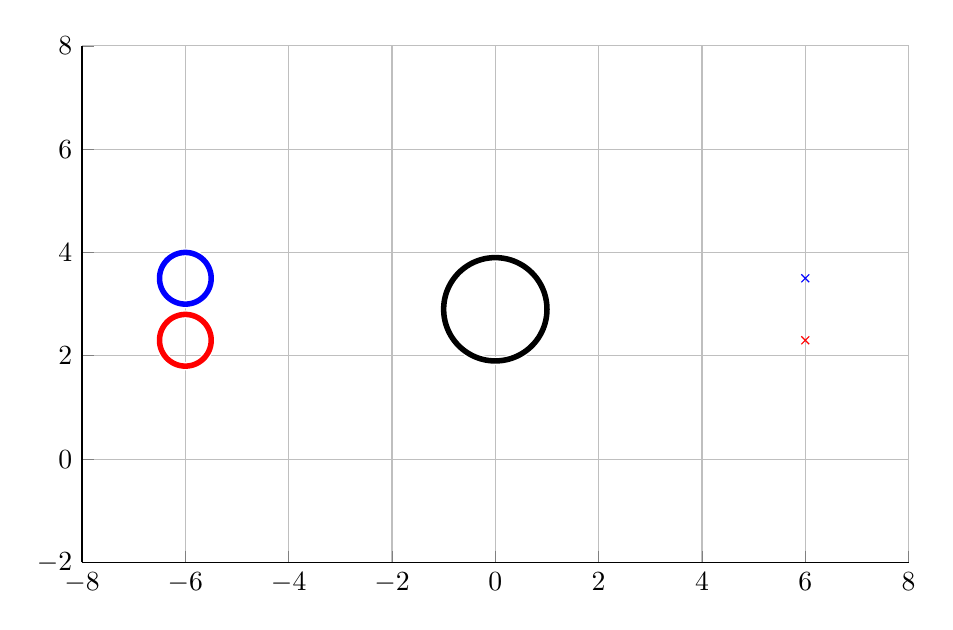
\begin{tikzpicture}

\begin{axis}[%
width=4.133in,
height=2.583in,
at={(0.693in,0.778in)},
scale only axis,
unbounded coords=jump,
xmin=-8,
xmax=8,
xmajorgrids,
ymin=-2,
ymax=8,
ymajorgrids,
axis background/.style={fill=white},
axis x line*=bottom,
axis y line*=left
]
\addplot [color=blue,only marks,mark=x,mark options={solid},forget plot]
  table[row sep=crcr]{%
6	3.5\\
};
\addplot [color=red,only marks,mark=x,mark options={solid},forget plot]
  table[row sep=crcr]{%
6	2.3\\
};
\addplot [color=white,solid,line width=3.0pt,forget plot]
  table[row sep=crcr]{%
-5.5	3.5\\
-5.50030458649045	3.51744974835125\\
-5.50121797487009	3.53487823687206\\
-5.50273905231586	3.55226423163383\\
-5.50486596562921	3.56958655048003\\
-5.5075961234939	3.58682408883347\\
-5.5109261996331	3.60395584540888\\
-5.514852136862	3.62096094779983\\
-5.51936915203084	3.6378186779085\\
-5.52447174185242	3.65450849718747\\
-5.53015368960705	3.67101007166283\\
-5.53640807271661	3.68730329670796\\
-5.5432272711787	3.7033683215379\\
-5.55060297685042	3.71918557339454\\
-5.55852620357054	3.73473578139295\\
-5.56698729810778	3.75\\
-5.57597595192179	3.7649596321166\\
-5.58548121372248	3.77959645173537\\
-5.59549150281253	3.79389262614624\\
-5.60599462319664	3.80783073766283\\
-5.61697777844051	3.82139380484327\\
-5.6284275872613	3.83456530317943\\
-5.64033009983067	3.8473291852295\\
-5.6526708147705	3.85966990016933\\
-5.66543469682057	3.8715724127387\\
-5.67860619515673	3.88302222155949\\
-5.69216926233717	3.89400537680336\\
-5.70610737385376	3.90450849718747\\
-5.72040354826463	3.91451878627752\\
-5.7350403678834	3.92402404807821\\
-5.75	3.93301270189222\\
-5.76526421860705	3.94147379642946\\
-5.78081442660546	3.94939702314958\\
-5.7966316784621	3.9567727288213\\
-5.81269670329204	3.96359192728339\\
-5.82898992833717	3.96984631039295\\
-5.84549150281253	3.97552825814758\\
-5.8621813220915	3.98063084796916\\
-5.87903905220017	3.985147863138\\
-5.89604415459112	3.9890738003669\\
-5.91317591116653	3.9924038765061\\
-5.93041344951997	3.99513403437079\\
-5.94773576836617	3.99726094768414\\
-5.96512176312794	3.99878202512991\\
-5.98255025164875	3.99969541350955\\
-6	4\\
-6.01744974835125	3.99969541350955\\
-6.03487823687206	3.99878202512991\\
-6.05226423163383	3.99726094768414\\
-6.06958655048003	3.99513403437079\\
-6.08682408883347	3.9924038765061\\
-6.10395584540888	3.9890738003669\\
-6.12096094779983	3.985147863138\\
-6.1378186779085	3.98063084796916\\
-6.15450849718747	3.97552825814758\\
-6.17101007166283	3.96984631039295\\
-6.18730329670796	3.96359192728339\\
-6.2033683215379	3.9567727288213\\
-6.21918557339454	3.94939702314958\\
-6.23473578139295	3.94147379642946\\
-6.25	3.93301270189222\\
-6.2649596321166	3.92402404807821\\
-6.27959645173537	3.91451878627752\\
-6.29389262614624	3.90450849718747\\
-6.30783073766283	3.89400537680336\\
-6.32139380484327	3.88302222155949\\
-6.33456530317943	3.8715724127387\\
-6.3473291852295	3.85966990016933\\
-6.35966990016933	3.8473291852295\\
-6.3715724127387	3.83456530317943\\
-6.38302222155949	3.82139380484327\\
-6.39400537680336	3.80783073766283\\
-6.40450849718747	3.79389262614624\\
-6.41451878627752	3.77959645173537\\
-6.42402404807821	3.7649596321166\\
-6.43301270189222	3.75\\
-6.44147379642946	3.73473578139295\\
-6.44939702314958	3.71918557339454\\
-6.4567727288213	3.7033683215379\\
-6.46359192728339	3.68730329670796\\
-6.46984631039295	3.67101007166283\\
-6.47552825814758	3.65450849718747\\
-6.48063084796916	3.6378186779085\\
-6.485147863138	3.62096094779983\\
-6.4890738003669	3.60395584540888\\
-6.4924038765061	3.58682408883347\\
-6.49513403437079	3.56958655048003\\
-6.49726094768414	3.55226423163383\\
-6.49878202512991	3.53487823687206\\
-6.49969541350955	3.51744974835125\\
-6.5	3.5\\
-6.49969541350955	3.48255025164875\\
-6.49878202512991	3.46512176312794\\
-6.49726094768414	3.44773576836617\\
-6.49513403437079	3.43041344951997\\
-6.4924038765061	3.41317591116653\\
-6.4890738003669	3.39604415459112\\
-6.485147863138	3.37903905220017\\
-6.48063084796916	3.3621813220915\\
-6.47552825814758	3.34549150281253\\
-6.46984631039295	3.32898992833717\\
-6.46359192728339	3.31269670329204\\
-6.4567727288213	3.2966316784621\\
-6.44939702314958	3.28081442660546\\
-6.44147379642946	3.26526421860705\\
-6.43301270189222	3.25\\
-6.42402404807821	3.2350403678834\\
-6.41451878627752	3.22040354826463\\
-6.40450849718747	3.20610737385376\\
-6.39400537680336	3.19216926233717\\
-6.38302222155949	3.17860619515673\\
-6.3715724127387	3.16543469682057\\
-6.35966990016933	3.1526708147705\\
-6.3473291852295	3.14033009983067\\
-6.33456530317943	3.1284275872613\\
-6.32139380484327	3.11697777844051\\
-6.30783073766283	3.10599462319664\\
-6.29389262614624	3.09549150281253\\
-6.27959645173537	3.08548121372248\\
-6.2649596321166	3.07597595192179\\
-6.25	3.06698729810778\\
-6.23473578139295	3.05852620357054\\
-6.21918557339454	3.05060297685042\\
-6.2033683215379	3.0432272711787\\
-6.18730329670796	3.03640807271661\\
-6.17101007166283	3.03015368960705\\
-6.15450849718747	3.02447174185242\\
-6.1378186779085	3.01936915203084\\
-6.12096094779983	3.014852136862\\
-6.10395584540888	3.0109261996331\\
-6.08682408883347	3.0075961234939\\
-6.06958655048003	3.00486596562921\\
-6.05226423163383	3.00273905231586\\
-6.03487823687206	3.00121797487009\\
-6.01744974835125	3.00030458649045\\
-6	3\\
-5.98255025164875	3.00030458649045\\
-5.96512176312794	3.00121797487009\\
-5.94773576836617	3.00273905231586\\
-5.93041344951997	3.00486596562921\\
-5.91317591116653	3.0075961234939\\
-5.89604415459112	3.0109261996331\\
-5.87903905220017	3.014852136862\\
-5.8621813220915	3.01936915203084\\
-5.84549150281253	3.02447174185242\\
-5.82898992833717	3.03015368960705\\
-5.81269670329204	3.03640807271661\\
-5.7966316784621	3.0432272711787\\
-5.78081442660546	3.05060297685042\\
-5.76526421860705	3.05852620357054\\
-5.75	3.06698729810778\\
-5.7350403678834	3.07597595192179\\
-5.72040354826463	3.08548121372248\\
-5.70610737385376	3.09549150281253\\
-5.69216926233717	3.10599462319664\\
-5.67860619515673	3.11697777844051\\
-5.66543469682057	3.1284275872613\\
-5.6526708147705	3.14033009983067\\
-5.64033009983067	3.1526708147705\\
-5.6284275872613	3.16543469682057\\
-5.61697777844051	3.17860619515673\\
-5.60599462319664	3.19216926233717\\
-5.59549150281253	3.20610737385376\\
-5.58548121372248	3.22040354826463\\
-5.57597595192179	3.2350403678834\\
-5.56698729810778	3.25\\
-5.55852620357054	3.26526421860705\\
-5.55060297685042	3.28081442660546\\
-5.5432272711787	3.2966316784621\\
-5.53640807271661	3.31269670329204\\
-5.53015368960705	3.32898992833717\\
-5.52447174185242	3.34549150281253\\
-5.51936915203084	3.3621813220915\\
-5.514852136862	3.37903905220017\\
-5.5109261996331	3.39604415459112\\
-5.5075961234939	3.41317591116653\\
-5.50486596562921	3.43041344951997\\
-5.50273905231586	3.44773576836617\\
-5.50121797487009	3.46512176312794\\
-5.50030458649045	3.48255025164875\\
-5.5	3.5\\
nan	nan\\
};
\addplot [color=blue,solid,line width=2.0pt,forget plot]
  table[row sep=crcr]{%
-5.5	3.5\\
-5.50030458649045	3.51744974835125\\
-5.50121797487009	3.53487823687206\\
-5.50273905231586	3.55226423163383\\
-5.50486596562921	3.56958655048003\\
-5.5075961234939	3.58682408883347\\
-5.5109261996331	3.60395584540888\\
-5.514852136862	3.62096094779983\\
-5.51936915203084	3.6378186779085\\
-5.52447174185242	3.65450849718747\\
-5.53015368960705	3.67101007166283\\
-5.53640807271661	3.68730329670796\\
-5.5432272711787	3.7033683215379\\
-5.55060297685042	3.71918557339454\\
-5.55852620357054	3.73473578139295\\
-5.56698729810778	3.75\\
-5.57597595192179	3.7649596321166\\
-5.58548121372248	3.77959645173537\\
-5.59549150281253	3.79389262614624\\
-5.60599462319664	3.80783073766283\\
-5.61697777844051	3.82139380484327\\
-5.6284275872613	3.83456530317943\\
-5.64033009983067	3.8473291852295\\
-5.6526708147705	3.85966990016933\\
-5.66543469682057	3.8715724127387\\
-5.67860619515673	3.88302222155949\\
-5.69216926233717	3.89400537680336\\
-5.70610737385376	3.90450849718747\\
-5.72040354826463	3.91451878627752\\
-5.7350403678834	3.92402404807821\\
-5.75	3.93301270189222\\
-5.76526421860705	3.94147379642946\\
-5.78081442660546	3.94939702314958\\
-5.7966316784621	3.9567727288213\\
-5.81269670329204	3.96359192728339\\
-5.82898992833717	3.96984631039295\\
-5.84549150281253	3.97552825814758\\
-5.8621813220915	3.98063084796916\\
-5.87903905220017	3.985147863138\\
-5.89604415459112	3.9890738003669\\
-5.91317591116653	3.9924038765061\\
-5.93041344951997	3.99513403437079\\
-5.94773576836617	3.99726094768414\\
-5.96512176312794	3.99878202512991\\
-5.98255025164875	3.99969541350955\\
-6	4\\
-6.01744974835125	3.99969541350955\\
-6.03487823687206	3.99878202512991\\
-6.05226423163383	3.99726094768414\\
-6.06958655048003	3.99513403437079\\
-6.08682408883347	3.9924038765061\\
-6.10395584540888	3.9890738003669\\
-6.12096094779983	3.985147863138\\
-6.1378186779085	3.98063084796916\\
-6.15450849718747	3.97552825814758\\
-6.17101007166283	3.96984631039295\\
-6.18730329670796	3.96359192728339\\
-6.2033683215379	3.9567727288213\\
-6.21918557339454	3.94939702314958\\
-6.23473578139295	3.94147379642946\\
-6.25	3.93301270189222\\
-6.2649596321166	3.92402404807821\\
-6.27959645173537	3.91451878627752\\
-6.29389262614624	3.90450849718747\\
-6.30783073766283	3.89400537680336\\
-6.32139380484327	3.88302222155949\\
-6.33456530317943	3.8715724127387\\
-6.3473291852295	3.85966990016933\\
-6.35966990016933	3.8473291852295\\
-6.3715724127387	3.83456530317943\\
-6.38302222155949	3.82139380484327\\
-6.39400537680336	3.80783073766283\\
-6.40450849718747	3.79389262614624\\
-6.41451878627752	3.77959645173537\\
-6.42402404807821	3.7649596321166\\
-6.43301270189222	3.75\\
-6.44147379642946	3.73473578139295\\
-6.44939702314958	3.71918557339454\\
-6.4567727288213	3.7033683215379\\
-6.46359192728339	3.68730329670796\\
-6.46984631039295	3.67101007166283\\
-6.47552825814758	3.65450849718747\\
-6.48063084796916	3.6378186779085\\
-6.485147863138	3.62096094779983\\
-6.4890738003669	3.60395584540888\\
-6.4924038765061	3.58682408883347\\
-6.49513403437079	3.56958655048003\\
-6.49726094768414	3.55226423163383\\
-6.49878202512991	3.53487823687206\\
-6.49969541350955	3.51744974835125\\
-6.5	3.5\\
-6.49969541350955	3.48255025164875\\
-6.49878202512991	3.46512176312794\\
-6.49726094768414	3.44773576836617\\
-6.49513403437079	3.43041344951997\\
-6.4924038765061	3.41317591116653\\
-6.4890738003669	3.39604415459112\\
-6.485147863138	3.37903905220017\\
-6.48063084796916	3.3621813220915\\
-6.47552825814758	3.34549150281253\\
-6.46984631039295	3.32898992833717\\
-6.46359192728339	3.31269670329204\\
-6.4567727288213	3.2966316784621\\
-6.44939702314958	3.28081442660546\\
-6.44147379642946	3.26526421860705\\
-6.43301270189222	3.25\\
-6.42402404807821	3.2350403678834\\
-6.41451878627752	3.22040354826463\\
-6.40450849718747	3.20610737385376\\
-6.39400537680336	3.19216926233717\\
-6.38302222155949	3.17860619515673\\
-6.3715724127387	3.16543469682057\\
-6.35966990016933	3.1526708147705\\
-6.3473291852295	3.14033009983067\\
-6.33456530317943	3.1284275872613\\
-6.32139380484327	3.11697777844051\\
-6.30783073766283	3.10599462319664\\
-6.29389262614624	3.09549150281253\\
-6.27959645173537	3.08548121372248\\
-6.2649596321166	3.07597595192179\\
-6.25	3.06698729810778\\
-6.23473578139295	3.05852620357054\\
-6.21918557339454	3.05060297685042\\
-6.2033683215379	3.0432272711787\\
-6.18730329670796	3.03640807271661\\
-6.17101007166283	3.03015368960705\\
-6.15450849718747	3.02447174185242\\
-6.1378186779085	3.01936915203084\\
-6.12096094779983	3.014852136862\\
-6.10395584540888	3.0109261996331\\
-6.08682408883347	3.0075961234939\\
-6.06958655048003	3.00486596562921\\
-6.05226423163383	3.00273905231586\\
-6.03487823687206	3.00121797487009\\
-6.01744974835125	3.00030458649045\\
-6	3\\
-5.98255025164875	3.00030458649045\\
-5.96512176312794	3.00121797487009\\
-5.94773576836617	3.00273905231586\\
-5.93041344951997	3.00486596562921\\
-5.91317591116653	3.0075961234939\\
-5.89604415459112	3.0109261996331\\
-5.87903905220017	3.014852136862\\
-5.8621813220915	3.01936915203084\\
-5.84549150281253	3.02447174185242\\
-5.82898992833717	3.03015368960705\\
-5.81269670329204	3.03640807271661\\
-5.7966316784621	3.0432272711787\\
-5.78081442660546	3.05060297685042\\
-5.76526421860705	3.05852620357054\\
-5.75	3.06698729810778\\
-5.7350403678834	3.07597595192179\\
-5.72040354826463	3.08548121372248\\
-5.70610737385376	3.09549150281253\\
-5.69216926233717	3.10599462319664\\
-5.67860619515673	3.11697777844051\\
-5.66543469682057	3.1284275872613\\
-5.6526708147705	3.14033009983067\\
-5.64033009983067	3.1526708147705\\
-5.6284275872613	3.16543469682057\\
-5.61697777844051	3.17860619515673\\
-5.60599462319664	3.19216926233717\\
-5.59549150281253	3.20610737385376\\
-5.58548121372248	3.22040354826463\\
-5.57597595192179	3.2350403678834\\
-5.56698729810778	3.25\\
-5.55852620357054	3.26526421860705\\
-5.55060297685042	3.28081442660546\\
-5.5432272711787	3.2966316784621\\
-5.53640807271661	3.31269670329204\\
-5.53015368960705	3.32898992833717\\
-5.52447174185242	3.34549150281253\\
-5.51936915203084	3.3621813220915\\
-5.514852136862	3.37903905220017\\
-5.5109261996331	3.39604415459112\\
-5.5075961234939	3.41317591116653\\
-5.50486596562921	3.43041344951997\\
-5.50273905231586	3.44773576836617\\
-5.50121797487009	3.46512176312794\\
-5.50030458649045	3.48255025164875\\
-5.5	3.5\\
nan	nan\\
};
\addplot [color=white,solid,line width=3.0pt,forget plot]
  table[row sep=crcr]{%
-5.5	2.3\\
-5.50030458649045	2.31744974835125\\
-5.50121797487009	2.33487823687206\\
-5.50273905231586	2.35226423163383\\
-5.50486596562921	2.36958655048003\\
-5.5075961234939	2.38682408883346\\
-5.5109261996331	2.40395584540888\\
-5.514852136862	2.42096094779983\\
-5.51936915203084	2.4378186779085\\
-5.52447174185242	2.45450849718747\\
-5.53015368960705	2.47101007166283\\
-5.53640807271661	2.48730329670796\\
-5.5432272711787	2.5033683215379\\
-5.55060297685042	2.51918557339454\\
-5.55852620357054	2.53473578139295\\
-5.56698729810778	2.55\\
-5.57597595192179	2.5649596321166\\
-5.58548121372248	2.57959645173537\\
-5.59549150281253	2.59389262614624\\
-5.60599462319664	2.60783073766283\\
-5.61697777844051	2.62139380484327\\
-5.6284275872613	2.63456530317943\\
-5.64033009983067	2.6473291852295\\
-5.6526708147705	2.65966990016933\\
-5.66543469682057	2.6715724127387\\
-5.67860619515673	2.68302222155949\\
-5.69216926233717	2.69400537680336\\
-5.70610737385376	2.70450849718747\\
-5.72040354826463	2.71451878627752\\
-5.7350403678834	2.72402404807821\\
-5.75	2.73301270189222\\
-5.76526421860705	2.74147379642946\\
-5.78081442660546	2.74939702314958\\
-5.7966316784621	2.7567727288213\\
-5.81269670329204	2.76359192728339\\
-5.82898992833717	2.76984631039295\\
-5.84549150281253	2.77552825814758\\
-5.8621813220915	2.78063084796916\\
-5.87903905220017	2.785147863138\\
-5.89604415459112	2.7890738003669\\
-5.91317591116653	2.7924038765061\\
-5.93041344951997	2.79513403437078\\
-5.94773576836617	2.79726094768414\\
-5.96512176312794	2.79878202512991\\
-5.98255025164875	2.79969541350955\\
-6	2.8\\
-6.01744974835125	2.79969541350955\\
-6.03487823687206	2.79878202512991\\
-6.05226423163383	2.79726094768414\\
-6.06958655048003	2.79513403437078\\
-6.08682408883347	2.7924038765061\\
-6.10395584540888	2.7890738003669\\
-6.12096094779983	2.785147863138\\
-6.1378186779085	2.78063084796916\\
-6.15450849718747	2.77552825814758\\
-6.17101007166283	2.76984631039295\\
-6.18730329670796	2.76359192728339\\
-6.2033683215379	2.7567727288213\\
-6.21918557339454	2.74939702314958\\
-6.23473578139295	2.74147379642946\\
-6.25	2.73301270189222\\
-6.2649596321166	2.72402404807821\\
-6.27959645173537	2.71451878627752\\
-6.29389262614624	2.70450849718747\\
-6.30783073766283	2.69400537680336\\
-6.32139380484327	2.68302222155949\\
-6.33456530317943	2.6715724127387\\
-6.3473291852295	2.65966990016933\\
-6.35966990016933	2.6473291852295\\
-6.3715724127387	2.63456530317943\\
-6.38302222155949	2.62139380484327\\
-6.39400537680336	2.60783073766283\\
-6.40450849718747	2.59389262614624\\
-6.41451878627752	2.57959645173537\\
-6.42402404807821	2.5649596321166\\
-6.43301270189222	2.55\\
-6.44147379642946	2.53473578139295\\
-6.44939702314958	2.51918557339454\\
-6.4567727288213	2.5033683215379\\
-6.46359192728339	2.48730329670796\\
-6.46984631039295	2.47101007166283\\
-6.47552825814758	2.45450849718747\\
-6.48063084796916	2.4378186779085\\
-6.485147863138	2.42096094779983\\
-6.4890738003669	2.40395584540888\\
-6.4924038765061	2.38682408883346\\
-6.49513403437079	2.36958655048003\\
-6.49726094768414	2.35226423163383\\
-6.49878202512991	2.33487823687206\\
-6.49969541350955	2.31744974835125\\
-6.5	2.3\\
-6.49969541350955	2.28255025164875\\
-6.49878202512991	2.26512176312794\\
-6.49726094768414	2.24773576836617\\
-6.49513403437079	2.23041344951997\\
-6.4924038765061	2.21317591116653\\
-6.4890738003669	2.19604415459112\\
-6.485147863138	2.17903905220017\\
-6.48063084796916	2.1621813220915\\
-6.47552825814758	2.14549150281253\\
-6.46984631039295	2.12898992833717\\
-6.46359192728339	2.11269670329204\\
-6.4567727288213	2.0966316784621\\
-6.44939702314958	2.08081442660546\\
-6.44147379642946	2.06526421860705\\
-6.43301270189222	2.05\\
-6.42402404807821	2.0350403678834\\
-6.41451878627752	2.02040354826463\\
-6.40450849718747	2.00610737385376\\
-6.39400537680336	1.99216926233717\\
-6.38302222155949	1.97860619515673\\
-6.3715724127387	1.96543469682057\\
-6.35966990016933	1.9526708147705\\
-6.3473291852295	1.94033009983067\\
-6.33456530317943	1.9284275872613\\
-6.32139380484327	1.91697777844051\\
-6.30783073766283	1.90599462319664\\
-6.29389262614624	1.89549150281253\\
-6.27959645173537	1.88548121372248\\
-6.2649596321166	1.87597595192179\\
-6.25	1.86698729810778\\
-6.23473578139295	1.85852620357054\\
-6.21918557339454	1.85060297685042\\
-6.2033683215379	1.8432272711787\\
-6.18730329670796	1.83640807271661\\
-6.17101007166283	1.83015368960705\\
-6.15450849718747	1.82447174185242\\
-6.1378186779085	1.81936915203084\\
-6.12096094779983	1.814852136862\\
-6.10395584540888	1.8109261996331\\
-6.08682408883347	1.8075961234939\\
-6.06958655048003	1.80486596562921\\
-6.05226423163383	1.80273905231586\\
-6.03487823687206	1.80121797487009\\
-6.01744974835125	1.80030458649045\\
-6	1.8\\
-5.98255025164875	1.80030458649045\\
-5.96512176312794	1.80121797487009\\
-5.94773576836617	1.80273905231586\\
-5.93041344951997	1.80486596562921\\
-5.91317591116653	1.8075961234939\\
-5.89604415459112	1.8109261996331\\
-5.87903905220017	1.814852136862\\
-5.8621813220915	1.81936915203084\\
-5.84549150281253	1.82447174185242\\
-5.82898992833717	1.83015368960705\\
-5.81269670329204	1.83640807271661\\
-5.7966316784621	1.8432272711787\\
-5.78081442660546	1.85060297685042\\
-5.76526421860705	1.85852620357054\\
-5.75	1.86698729810778\\
-5.7350403678834	1.87597595192179\\
-5.72040354826463	1.88548121372248\\
-5.70610737385376	1.89549150281253\\
-5.69216926233717	1.90599462319664\\
-5.67860619515673	1.91697777844051\\
-5.66543469682057	1.9284275872613\\
-5.6526708147705	1.94033009983067\\
-5.64033009983067	1.9526708147705\\
-5.6284275872613	1.96543469682057\\
-5.61697777844051	1.97860619515673\\
-5.60599462319664	1.99216926233717\\
-5.59549150281253	2.00610737385376\\
-5.58548121372248	2.02040354826463\\
-5.57597595192179	2.0350403678834\\
-5.56698729810778	2.05\\
-5.55852620357054	2.06526421860705\\
-5.55060297685042	2.08081442660546\\
-5.5432272711787	2.0966316784621\\
-5.53640807271661	2.11269670329204\\
-5.53015368960705	2.12898992833717\\
-5.52447174185242	2.14549150281253\\
-5.51936915203084	2.1621813220915\\
-5.514852136862	2.17903905220017\\
-5.5109261996331	2.19604415459112\\
-5.5075961234939	2.21317591116653\\
-5.50486596562921	2.23041344951997\\
-5.50273905231586	2.24773576836617\\
-5.50121797487009	2.26512176312794\\
-5.50030458649045	2.28255025164875\\
-5.5	2.3\\
nan	nan\\
};
\addplot [color=red,solid,line width=2.0pt,forget plot]
  table[row sep=crcr]{%
-5.5	2.3\\
-5.50030458649045	2.31744974835125\\
-5.50121797487009	2.33487823687206\\
-5.50273905231586	2.35226423163383\\
-5.50486596562921	2.36958655048003\\
-5.5075961234939	2.38682408883346\\
-5.5109261996331	2.40395584540888\\
-5.514852136862	2.42096094779983\\
-5.51936915203084	2.4378186779085\\
-5.52447174185242	2.45450849718747\\
-5.53015368960705	2.47101007166283\\
-5.53640807271661	2.48730329670796\\
-5.5432272711787	2.5033683215379\\
-5.55060297685042	2.51918557339454\\
-5.55852620357054	2.53473578139295\\
-5.56698729810778	2.55\\
-5.57597595192179	2.5649596321166\\
-5.58548121372248	2.57959645173537\\
-5.59549150281253	2.59389262614624\\
-5.60599462319664	2.60783073766283\\
-5.61697777844051	2.62139380484327\\
-5.6284275872613	2.63456530317943\\
-5.64033009983067	2.6473291852295\\
-5.6526708147705	2.65966990016933\\
-5.66543469682057	2.6715724127387\\
-5.67860619515673	2.68302222155949\\
-5.69216926233717	2.69400537680336\\
-5.70610737385376	2.70450849718747\\
-5.72040354826463	2.71451878627752\\
-5.7350403678834	2.72402404807821\\
-5.75	2.73301270189222\\
-5.76526421860705	2.74147379642946\\
-5.78081442660546	2.74939702314958\\
-5.7966316784621	2.7567727288213\\
-5.81269670329204	2.76359192728339\\
-5.82898992833717	2.76984631039295\\
-5.84549150281253	2.77552825814758\\
-5.8621813220915	2.78063084796916\\
-5.87903905220017	2.785147863138\\
-5.89604415459112	2.7890738003669\\
-5.91317591116653	2.7924038765061\\
-5.93041344951997	2.79513403437078\\
-5.94773576836617	2.79726094768414\\
-5.96512176312794	2.79878202512991\\
-5.98255025164875	2.79969541350955\\
-6	2.8\\
-6.01744974835125	2.79969541350955\\
-6.03487823687206	2.79878202512991\\
-6.05226423163383	2.79726094768414\\
-6.06958655048003	2.79513403437078\\
-6.08682408883347	2.7924038765061\\
-6.10395584540888	2.7890738003669\\
-6.12096094779983	2.785147863138\\
-6.1378186779085	2.78063084796916\\
-6.15450849718747	2.77552825814758\\
-6.17101007166283	2.76984631039295\\
-6.18730329670796	2.76359192728339\\
-6.2033683215379	2.7567727288213\\
-6.21918557339454	2.74939702314958\\
-6.23473578139295	2.74147379642946\\
-6.25	2.73301270189222\\
-6.2649596321166	2.72402404807821\\
-6.27959645173537	2.71451878627752\\
-6.29389262614624	2.70450849718747\\
-6.30783073766283	2.69400537680336\\
-6.32139380484327	2.68302222155949\\
-6.33456530317943	2.6715724127387\\
-6.3473291852295	2.65966990016933\\
-6.35966990016933	2.6473291852295\\
-6.3715724127387	2.63456530317943\\
-6.38302222155949	2.62139380484327\\
-6.39400537680336	2.60783073766283\\
-6.40450849718747	2.59389262614624\\
-6.41451878627752	2.57959645173537\\
-6.42402404807821	2.5649596321166\\
-6.43301270189222	2.55\\
-6.44147379642946	2.53473578139295\\
-6.44939702314958	2.51918557339454\\
-6.4567727288213	2.5033683215379\\
-6.46359192728339	2.48730329670796\\
-6.46984631039295	2.47101007166283\\
-6.47552825814758	2.45450849718747\\
-6.48063084796916	2.4378186779085\\
-6.485147863138	2.42096094779983\\
-6.4890738003669	2.40395584540888\\
-6.4924038765061	2.38682408883346\\
-6.49513403437079	2.36958655048003\\
-6.49726094768414	2.35226423163383\\
-6.49878202512991	2.33487823687206\\
-6.49969541350955	2.31744974835125\\
-6.5	2.3\\
-6.49969541350955	2.28255025164875\\
-6.49878202512991	2.26512176312794\\
-6.49726094768414	2.24773576836617\\
-6.49513403437079	2.23041344951997\\
-6.4924038765061	2.21317591116653\\
-6.4890738003669	2.19604415459112\\
-6.485147863138	2.17903905220017\\
-6.48063084796916	2.1621813220915\\
-6.47552825814758	2.14549150281253\\
-6.46984631039295	2.12898992833717\\
-6.46359192728339	2.11269670329204\\
-6.4567727288213	2.0966316784621\\
-6.44939702314958	2.08081442660546\\
-6.44147379642946	2.06526421860705\\
-6.43301270189222	2.05\\
-6.42402404807821	2.0350403678834\\
-6.41451878627752	2.02040354826463\\
-6.40450849718747	2.00610737385376\\
-6.39400537680336	1.99216926233717\\
-6.38302222155949	1.97860619515673\\
-6.3715724127387	1.96543469682057\\
-6.35966990016933	1.9526708147705\\
-6.3473291852295	1.94033009983067\\
-6.33456530317943	1.9284275872613\\
-6.32139380484327	1.91697777844051\\
-6.30783073766283	1.90599462319664\\
-6.29389262614624	1.89549150281253\\
-6.27959645173537	1.88548121372248\\
-6.2649596321166	1.87597595192179\\
-6.25	1.86698729810778\\
-6.23473578139295	1.85852620357054\\
-6.21918557339454	1.85060297685042\\
-6.2033683215379	1.8432272711787\\
-6.18730329670796	1.83640807271661\\
-6.17101007166283	1.83015368960705\\
-6.15450849718747	1.82447174185242\\
-6.1378186779085	1.81936915203084\\
-6.12096094779983	1.814852136862\\
-6.10395584540888	1.8109261996331\\
-6.08682408883347	1.8075961234939\\
-6.06958655048003	1.80486596562921\\
-6.05226423163383	1.80273905231586\\
-6.03487823687206	1.80121797487009\\
-6.01744974835125	1.80030458649045\\
-6	1.8\\
-5.98255025164875	1.80030458649045\\
-5.96512176312794	1.80121797487009\\
-5.94773576836617	1.80273905231586\\
-5.93041344951997	1.80486596562921\\
-5.91317591116653	1.8075961234939\\
-5.89604415459112	1.8109261996331\\
-5.87903905220017	1.814852136862\\
-5.8621813220915	1.81936915203084\\
-5.84549150281253	1.82447174185242\\
-5.82898992833717	1.83015368960705\\
-5.81269670329204	1.83640807271661\\
-5.7966316784621	1.8432272711787\\
-5.78081442660546	1.85060297685042\\
-5.76526421860705	1.85852620357054\\
-5.75	1.86698729810778\\
-5.7350403678834	1.87597595192179\\
-5.72040354826463	1.88548121372248\\
-5.70610737385376	1.89549150281253\\
-5.69216926233717	1.90599462319664\\
-5.67860619515673	1.91697777844051\\
-5.66543469682057	1.9284275872613\\
-5.6526708147705	1.94033009983067\\
-5.64033009983067	1.9526708147705\\
-5.6284275872613	1.96543469682057\\
-5.61697777844051	1.97860619515673\\
-5.60599462319664	1.99216926233717\\
-5.59549150281253	2.00610737385376\\
-5.58548121372248	2.02040354826463\\
-5.57597595192179	2.0350403678834\\
-5.56698729810778	2.05\\
-5.55852620357054	2.06526421860705\\
-5.55060297685042	2.08081442660546\\
-5.5432272711787	2.0966316784621\\
-5.53640807271661	2.11269670329204\\
-5.53015368960705	2.12898992833717\\
-5.52447174185242	2.14549150281253\\
-5.51936915203084	2.1621813220915\\
-5.514852136862	2.17903905220017\\
-5.5109261996331	2.19604415459112\\
-5.5075961234939	2.21317591116653\\
-5.50486596562921	2.23041344951997\\
-5.50273905231586	2.24773576836617\\
-5.50121797487009	2.26512176312794\\
-5.50030458649045	2.28255025164875\\
-5.5	2.3\\
nan	nan\\
};
\addplot [color=white,solid,line width=3.0pt,forget plot]
  table[row sep=crcr]{%
1	2.9\\
0.999390827019096	2.9348994967025\\
0.997564050259824	2.96975647374413\\
0.994521895368273	3.00452846326765\\
0.99026806874157	3.03917310096007\\
0.984807753012208	3.07364817766693\\
0.978147600733806	3.10791169081776\\
0.970295726275996	3.14192189559967\\
0.961261695938319	3.175637355817\\
0.951056516295154	3.20901699437495\\
0.939692620785908	3.24202014332567\\
0.927183854566787	3.27460659341591\\
0.913545457642601	3.3067366430758\\
0.898794046299167	3.33837114678908\\
0.882947592858927	3.36947156278589\\
0.866025403784439	3.4\\
0.848048096156426	3.42991926423321\\
0.829037572555042	3.45919290347075\\
0.809016994374947	3.48778525229247\\
0.788010753606722	3.51566147532566\\
0.766044443118978	3.54278760968654\\
0.743144825477394	3.56913060635886\\
0.719339800338651	3.594658370459\\
0.694658370458997	3.61933980033865\\
0.669130606358858	3.64314482547739\\
0.642787609686539	3.66604444311898\\
0.615661475325658	3.68801075360672\\
0.587785252292473	3.70901699437495\\
0.559192903470747	3.72903757255504\\
0.529919264233205	3.74804809615643\\
0.5	3.76602540378444\\
0.469471562785891	3.78294759285893\\
0.438371146789077	3.79879404629917\\
0.4067366430758	3.8135454576426\\
0.374606593415912	3.82718385456679\\
0.342020143325669	3.83969262078591\\
0.309016994374947	3.85105651629515\\
0.275637355816999	3.86126169593832\\
0.241921895599668	3.870295726276\\
0.207911690817759	3.87814760073381\\
0.17364817766693	3.88480775301221\\
0.139173100960066	3.89026806874157\\
0.104528463267653	3.89452189536827\\
0.0697564737441255	3.89756405025982\\
0.0348994967025011	3.8993908270191\\
6.12323399573677e-17	3.9\\
-0.0348994967025007	3.8993908270191\\
-0.0697564737441253	3.89756405025982\\
-0.104528463267653	3.89452189536827\\
-0.139173100960065	3.89026806874157\\
-0.17364817766693	3.88480775301221\\
-0.207911690817759	3.87814760073381\\
-0.241921895599668	3.870295726276\\
-0.275637355816999	3.86126169593832\\
-0.309016994374947	3.85105651629515\\
-0.342020143325669	3.83969262078591\\
-0.374606593415912	3.82718385456679\\
-0.4067366430758	3.8135454576426\\
-0.438371146789078	3.79879404629917\\
-0.469471562785891	3.78294759285893\\
-0.5	3.76602540378444\\
-0.529919264233205	3.74804809615643\\
-0.559192903470747	3.72903757255504\\
-0.587785252292473	3.70901699437495\\
-0.615661475325658	3.68801075360672\\
-0.642787609686539	3.66604444311898\\
-0.669130606358858	3.64314482547739\\
-0.694658370458997	3.61933980033865\\
-0.719339800338651	3.594658370459\\
-0.743144825477394	3.56913060635886\\
-0.766044443118978	3.54278760968654\\
-0.788010753606722	3.51566147532566\\
-0.809016994374947	3.48778525229247\\
-0.829037572555042	3.45919290347075\\
-0.848048096156426	3.42991926423321\\
-0.866025403784439	3.4\\
-0.882947592858927	3.36947156278589\\
-0.898794046299167	3.33837114678908\\
-0.913545457642601	3.3067366430758\\
-0.927183854566787	3.27460659341591\\
-0.939692620785908	3.24202014332567\\
-0.951056516295154	3.20901699437495\\
-0.961261695938319	3.175637355817\\
-0.970295726275996	3.14192189559967\\
-0.978147600733806	3.10791169081776\\
-0.984807753012208	3.07364817766693\\
-0.99026806874157	3.03917310096007\\
-0.994521895368273	3.00452846326765\\
-0.997564050259824	2.96975647374413\\
-0.999390827019096	2.9348994967025\\
-1	2.9\\
-0.999390827019096	2.8651005032975\\
-0.997564050259824	2.83024352625588\\
-0.994521895368273	2.79547153673235\\
-0.99026806874157	2.76082689903993\\
-0.984807753012208	2.72635182233307\\
-0.978147600733806	2.69208830918224\\
-0.970295726275997	2.65807810440033\\
-0.961261695938319	2.624362644183\\
-0.951056516295154	2.59098300562505\\
-0.939692620785908	2.55797985667433\\
-0.927183854566787	2.52539340658409\\
-0.913545457642601	2.4932633569242\\
-0.898794046299167	2.46162885321092\\
-0.882947592858927	2.43052843721411\\
-0.866025403784439	2.4\\
-0.848048096156426	2.3700807357668\\
-0.829037572555042	2.34080709652925\\
-0.809016994374947	2.31221474770753\\
-0.788010753606722	2.28433852467434\\
-0.766044443118978	2.25721239031346\\
-0.743144825477394	2.23086939364114\\
-0.719339800338651	2.205341629541\\
-0.694658370458997	2.18066019966135\\
-0.669130606358858	2.15685517452261\\
-0.642787609686539	2.13395555688102\\
-0.615661475325658	2.11198924639328\\
-0.587785252292473	2.09098300562505\\
-0.559192903470747	2.07096242744496\\
-0.529919264233205	2.05195190384357\\
-0.5	2.03397459621556\\
-0.469471562785891	2.01705240714107\\
-0.438371146789078	2.00120595370083\\
-0.4067366430758	1.9864545423574\\
-0.374606593415912	1.97281614543321\\
-0.342020143325669	1.96030737921409\\
-0.309016994374948	1.94894348370485\\
-0.275637355816999	1.93873830406168\\
-0.241921895599668	1.929704273724\\
-0.20791169081776	1.92185239926619\\
-0.17364817766693	1.91519224698779\\
-0.139173100960065	1.90973193125843\\
-0.104528463267653	1.90547810463173\\
-0.0697564737441256	1.90243594974018\\
-0.0348994967025016	1.9006091729809\\
-1.83697019872103e-16	1.9\\
0.0348994967025013	1.9006091729809\\
0.0697564737441252	1.90243594974018\\
0.104528463267653	1.90547810463173\\
0.139173100960065	1.90973193125843\\
0.17364817766693	1.91519224698779\\
0.207911690817759	1.92185239926619\\
0.241921895599667	1.929704273724\\
0.275637355816999	1.93873830406168\\
0.309016994374947	1.94894348370485\\
0.342020143325668	1.96030737921409\\
0.374606593415912	1.97281614543321\\
0.406736643075801	1.9864545423574\\
0.438371146789077	2.00120595370083\\
0.46947156278589	2.01705240714107\\
0.5	2.03397459621556\\
0.529919264233205	2.05195190384357\\
0.559192903470746	2.07096242744496\\
0.587785252292473	2.09098300562505\\
0.615661475325659	2.11198924639328\\
0.642787609686539	2.13395555688102\\
0.669130606358858	2.15685517452261\\
0.694658370458997	2.18066019966135\\
0.719339800338651	2.205341629541\\
0.743144825477394	2.23086939364114\\
0.766044443118978	2.25721239031346\\
0.788010753606722	2.28433852467434\\
0.809016994374947	2.31221474770753\\
0.829037572555041	2.34080709652925\\
0.848048096156425	2.37008073576679\\
0.866025403784438	2.4\\
0.882947592858927	2.43052843721411\\
0.898794046299167	2.46162885321092\\
0.913545457642601	2.4932633569242\\
0.927183854566787	2.52539340658409\\
0.939692620785908	2.55797985667433\\
0.951056516295154	2.59098300562505\\
0.961261695938319	2.624362644183\\
0.970295726275996	2.65807810440033\\
0.978147600733806	2.69208830918224\\
0.984807753012208	2.72635182233307\\
0.99026806874157	2.76082689903993\\
0.994521895368273	2.79547153673235\\
0.997564050259824	2.83024352625588\\
0.999390827019096	2.8651005032975\\
1	2.9\\
nan	nan\\
};
\addplot [color=black,solid,line width=2.0pt,forget plot]
  table[row sep=crcr]{%
1	2.9\\
0.999390827019096	2.9348994967025\\
0.997564050259824	2.96975647374413\\
0.994521895368273	3.00452846326765\\
0.99026806874157	3.03917310096007\\
0.984807753012208	3.07364817766693\\
0.978147600733806	3.10791169081776\\
0.970295726275996	3.14192189559967\\
0.961261695938319	3.175637355817\\
0.951056516295154	3.20901699437495\\
0.939692620785908	3.24202014332567\\
0.927183854566787	3.27460659341591\\
0.913545457642601	3.3067366430758\\
0.898794046299167	3.33837114678908\\
0.882947592858927	3.36947156278589\\
0.866025403784439	3.4\\
0.848048096156426	3.42991926423321\\
0.829037572555042	3.45919290347075\\
0.809016994374947	3.48778525229247\\
0.788010753606722	3.51566147532566\\
0.766044443118978	3.54278760968654\\
0.743144825477394	3.56913060635886\\
0.719339800338651	3.594658370459\\
0.694658370458997	3.61933980033865\\
0.669130606358858	3.64314482547739\\
0.642787609686539	3.66604444311898\\
0.615661475325658	3.68801075360672\\
0.587785252292473	3.70901699437495\\
0.559192903470747	3.72903757255504\\
0.529919264233205	3.74804809615643\\
0.5	3.76602540378444\\
0.469471562785891	3.78294759285893\\
0.438371146789077	3.79879404629917\\
0.4067366430758	3.8135454576426\\
0.374606593415912	3.82718385456679\\
0.342020143325669	3.83969262078591\\
0.309016994374947	3.85105651629515\\
0.275637355816999	3.86126169593832\\
0.241921895599668	3.870295726276\\
0.207911690817759	3.87814760073381\\
0.17364817766693	3.88480775301221\\
0.139173100960066	3.89026806874157\\
0.104528463267653	3.89452189536827\\
0.0697564737441255	3.89756405025982\\
0.0348994967025011	3.8993908270191\\
6.12323399573677e-17	3.9\\
-0.0348994967025007	3.8993908270191\\
-0.0697564737441253	3.89756405025982\\
-0.104528463267653	3.89452189536827\\
-0.139173100960065	3.89026806874157\\
-0.17364817766693	3.88480775301221\\
-0.207911690817759	3.87814760073381\\
-0.241921895599668	3.870295726276\\
-0.275637355816999	3.86126169593832\\
-0.309016994374947	3.85105651629515\\
-0.342020143325669	3.83969262078591\\
-0.374606593415912	3.82718385456679\\
-0.4067366430758	3.8135454576426\\
-0.438371146789078	3.79879404629917\\
-0.469471562785891	3.78294759285893\\
-0.5	3.76602540378444\\
-0.529919264233205	3.74804809615643\\
-0.559192903470747	3.72903757255504\\
-0.587785252292473	3.70901699437495\\
-0.615661475325658	3.68801075360672\\
-0.642787609686539	3.66604444311898\\
-0.669130606358858	3.64314482547739\\
-0.694658370458997	3.61933980033865\\
-0.719339800338651	3.594658370459\\
-0.743144825477394	3.56913060635886\\
-0.766044443118978	3.54278760968654\\
-0.788010753606722	3.51566147532566\\
-0.809016994374947	3.48778525229247\\
-0.829037572555042	3.45919290347075\\
-0.848048096156426	3.42991926423321\\
-0.866025403784439	3.4\\
-0.882947592858927	3.36947156278589\\
-0.898794046299167	3.33837114678908\\
-0.913545457642601	3.3067366430758\\
-0.927183854566787	3.27460659341591\\
-0.939692620785908	3.24202014332567\\
-0.951056516295154	3.20901699437495\\
-0.961261695938319	3.175637355817\\
-0.970295726275996	3.14192189559967\\
-0.978147600733806	3.10791169081776\\
-0.984807753012208	3.07364817766693\\
-0.99026806874157	3.03917310096007\\
-0.994521895368273	3.00452846326765\\
-0.997564050259824	2.96975647374413\\
-0.999390827019096	2.9348994967025\\
-1	2.9\\
-0.999390827019096	2.8651005032975\\
-0.997564050259824	2.83024352625588\\
-0.994521895368273	2.79547153673235\\
-0.99026806874157	2.76082689903993\\
-0.984807753012208	2.72635182233307\\
-0.978147600733806	2.69208830918224\\
-0.970295726275997	2.65807810440033\\
-0.961261695938319	2.624362644183\\
-0.951056516295154	2.59098300562505\\
-0.939692620785908	2.55797985667433\\
-0.927183854566787	2.52539340658409\\
-0.913545457642601	2.4932633569242\\
-0.898794046299167	2.46162885321092\\
-0.882947592858927	2.43052843721411\\
-0.866025403784439	2.4\\
-0.848048096156426	2.3700807357668\\
-0.829037572555042	2.34080709652925\\
-0.809016994374947	2.31221474770753\\
-0.788010753606722	2.28433852467434\\
-0.766044443118978	2.25721239031346\\
-0.743144825477394	2.23086939364114\\
-0.719339800338651	2.205341629541\\
-0.694658370458997	2.18066019966135\\
-0.669130606358858	2.15685517452261\\
-0.642787609686539	2.13395555688102\\
-0.615661475325658	2.11198924639328\\
-0.587785252292473	2.09098300562505\\
-0.559192903470747	2.07096242744496\\
-0.529919264233205	2.05195190384357\\
-0.5	2.03397459621556\\
-0.469471562785891	2.01705240714107\\
-0.438371146789078	2.00120595370083\\
-0.4067366430758	1.9864545423574\\
-0.374606593415912	1.97281614543321\\
-0.342020143325669	1.96030737921409\\
-0.309016994374948	1.94894348370485\\
-0.275637355816999	1.93873830406168\\
-0.241921895599668	1.929704273724\\
-0.20791169081776	1.92185239926619\\
-0.17364817766693	1.91519224698779\\
-0.139173100960065	1.90973193125843\\
-0.104528463267653	1.90547810463173\\
-0.0697564737441256	1.90243594974018\\
-0.0348994967025016	1.9006091729809\\
-1.83697019872103e-16	1.9\\
0.0348994967025013	1.9006091729809\\
0.0697564737441252	1.90243594974018\\
0.104528463267653	1.90547810463173\\
0.139173100960065	1.90973193125843\\
0.17364817766693	1.91519224698779\\
0.207911690817759	1.92185239926619\\
0.241921895599667	1.929704273724\\
0.275637355816999	1.93873830406168\\
0.309016994374947	1.94894348370485\\
0.342020143325668	1.96030737921409\\
0.374606593415912	1.97281614543321\\
0.406736643075801	1.9864545423574\\
0.438371146789077	2.00120595370083\\
0.46947156278589	2.01705240714107\\
0.5	2.03397459621556\\
0.529919264233205	2.05195190384357\\
0.559192903470746	2.07096242744496\\
0.587785252292473	2.09098300562505\\
0.615661475325659	2.11198924639328\\
0.642787609686539	2.13395555688102\\
0.669130606358858	2.15685517452261\\
0.694658370458997	2.18066019966135\\
0.719339800338651	2.205341629541\\
0.743144825477394	2.23086939364114\\
0.766044443118978	2.25721239031346\\
0.788010753606722	2.28433852467434\\
0.809016994374947	2.31221474770753\\
0.829037572555041	2.34080709652925\\
0.848048096156425	2.37008073576679\\
0.866025403784438	2.4\\
0.882947592858927	2.43052843721411\\
0.898794046299167	2.46162885321092\\
0.913545457642601	2.4932633569242\\
0.927183854566787	2.52539340658409\\
0.939692620785908	2.55797985667433\\
0.951056516295154	2.59098300562505\\
0.961261695938319	2.624362644183\\
0.970295726275996	2.65807810440033\\
0.978147600733806	2.69208830918224\\
0.984807753012208	2.72635182233307\\
0.99026806874157	2.76082689903993\\
0.994521895368273	2.79547153673235\\
0.997564050259824	2.83024352625588\\
0.999390827019096	2.8651005032975\\
1	2.9\\
nan	nan\\
};
\end{axis}
\end{tikzpicture}%}
      \caption{Test case one: two agents and one obstacle.}
      \label{fig:test_case_2_1}
    \end{figure}
  \end{minipage}
  \hfill
  \begin{minipage}{0.45\linewidth}
    \begin{figure}[H]
      \scalebox{0.7}{% This file was created by matlab2tikz.
%
%The latest updates can be retrieved from
%  http://www.mathworks.com/matlabcentral/fileexchange/22022-matlab2tikz-matlab2tikz
%where you can also make suggestions and rate matlab2tikz.
%
\begin{tikzpicture}

\definecolor{mycolor1}{rgb}{0.00000,0.44700,0.74100}%
\definecolor{mycolor2}{rgb}{0.85000,0.32500,0.09800}%
\definecolor{mycolor3}{rgb}{0.92900,0.69400,0.12500}%

\begin{axis}[%
width=4.133in,
height=2.583in,
at={(0.693in,0.778in)},
scale only axis,
unbounded coords=jump,
xmin=-8,
xmax=8,
%xmajorgrids,
ymin=-1.5,
ymax=8.5,
%ymajorgrids,
axis background/.style={fill=white},
axis x line*=bottom,
axis y line*=left
]
\addplot [color=mycolor1,only marks,mark=x,mark options={solid},forget plot]
  table[row sep=crcr]{%
6	4.25\\
};
\addplot [color=mycolor2,only marks,mark=x,mark options={solid},forget plot]
  table[row sep=crcr]{%
6	2.75\\
};
\addplot [color=white,solid,line width=3.0pt,forget plot]
  table[row sep=crcr]{%
-5.5	4.25\\
-5.50030458649045	4.26744974835125\\
-5.50121797487009	4.28487823687206\\
-5.50273905231586	4.30226423163383\\
-5.50486596562921	4.31958655048003\\
-5.5075961234939	4.33682408883347\\
-5.5109261996331	4.35395584540888\\
-5.514852136862	4.37096094779983\\
-5.51936915203084	4.3878186779085\\
-5.52447174185242	4.40450849718747\\
-5.53015368960705	4.42101007166283\\
-5.53640807271661	4.43730329670796\\
-5.5432272711787	4.4533683215379\\
-5.55060297685042	4.46918557339454\\
-5.55852620357054	4.48473578139295\\
-5.56698729810778	4.5\\
-5.57597595192179	4.5149596321166\\
-5.58548121372248	4.52959645173537\\
-5.59549150281253	4.54389262614624\\
-5.60599462319664	4.55783073766283\\
-5.61697777844051	4.57139380484327\\
-5.6284275872613	4.58456530317943\\
-5.64033009983067	4.5973291852295\\
-5.6526708147705	4.60966990016933\\
-5.66543469682057	4.6215724127387\\
-5.67860619515673	4.63302222155949\\
-5.69216926233717	4.64400537680336\\
-5.70610737385376	4.65450849718747\\
-5.72040354826463	4.66451878627752\\
-5.7350403678834	4.67402404807821\\
-5.75	4.68301270189222\\
-5.76526421860705	4.69147379642946\\
-5.78081442660546	4.69939702314958\\
-5.7966316784621	4.7067727288213\\
-5.81269670329204	4.71359192728339\\
-5.82898992833717	4.71984631039295\\
-5.84549150281253	4.72552825814758\\
-5.8621813220915	4.73063084796916\\
-5.87903905220017	4.735147863138\\
-5.89604415459112	4.7390738003669\\
-5.91317591116653	4.7424038765061\\
-5.93041344951997	4.74513403437079\\
-5.94773576836617	4.74726094768414\\
-5.96512176312794	4.74878202512991\\
-5.98255025164875	4.74969541350955\\
-6	4.75\\
-6.01744974835125	4.74969541350955\\
-6.03487823687206	4.74878202512991\\
-6.05226423163383	4.74726094768414\\
-6.06958655048003	4.74513403437079\\
-6.08682408883347	4.7424038765061\\
-6.10395584540888	4.7390738003669\\
-6.12096094779983	4.735147863138\\
-6.1378186779085	4.73063084796916\\
-6.15450849718747	4.72552825814758\\
-6.17101007166283	4.71984631039295\\
-6.18730329670796	4.71359192728339\\
-6.2033683215379	4.7067727288213\\
-6.21918557339454	4.69939702314958\\
-6.23473578139295	4.69147379642946\\
-6.25	4.68301270189222\\
-6.2649596321166	4.67402404807821\\
-6.27959645173537	4.66451878627752\\
-6.29389262614624	4.65450849718747\\
-6.30783073766283	4.64400537680336\\
-6.32139380484327	4.63302222155949\\
-6.33456530317943	4.6215724127387\\
-6.3473291852295	4.60966990016933\\
-6.35966990016933	4.5973291852295\\
-6.3715724127387	4.58456530317943\\
-6.38302222155949	4.57139380484327\\
-6.39400537680336	4.55783073766283\\
-6.40450849718747	4.54389262614624\\
-6.41451878627752	4.52959645173537\\
-6.42402404807821	4.5149596321166\\
-6.43301270189222	4.5\\
-6.44147379642946	4.48473578139295\\
-6.44939702314958	4.46918557339454\\
-6.4567727288213	4.4533683215379\\
-6.46359192728339	4.43730329670796\\
-6.46984631039295	4.42101007166283\\
-6.47552825814758	4.40450849718747\\
-6.48063084796916	4.3878186779085\\
-6.485147863138	4.37096094779983\\
-6.4890738003669	4.35395584540888\\
-6.4924038765061	4.33682408883347\\
-6.49513403437079	4.31958655048003\\
-6.49726094768414	4.30226423163383\\
-6.49878202512991	4.28487823687206\\
-6.49969541350955	4.26744974835125\\
-6.5	4.25\\
-6.49969541350955	4.23255025164875\\
-6.49878202512991	4.21512176312794\\
-6.49726094768414	4.19773576836617\\
-6.49513403437079	4.18041344951997\\
-6.4924038765061	4.16317591116653\\
-6.4890738003669	4.14604415459112\\
-6.485147863138	4.12903905220017\\
-6.48063084796916	4.1121813220915\\
-6.47552825814758	4.09549150281253\\
-6.46984631039295	4.07898992833717\\
-6.46359192728339	4.06269670329204\\
-6.4567727288213	4.0466316784621\\
-6.44939702314958	4.03081442660546\\
-6.44147379642946	4.01526421860705\\
-6.43301270189222	4\\
-6.42402404807821	3.9850403678834\\
-6.41451878627752	3.97040354826463\\
-6.40450849718747	3.95610737385376\\
-6.39400537680336	3.94216926233717\\
-6.38302222155949	3.92860619515673\\
-6.3715724127387	3.91543469682057\\
-6.35966990016933	3.9026708147705\\
-6.3473291852295	3.89033009983067\\
-6.33456530317943	3.8784275872613\\
-6.32139380484327	3.86697777844051\\
-6.30783073766283	3.85599462319664\\
-6.29389262614624	3.84549150281253\\
-6.27959645173537	3.83548121372248\\
-6.2649596321166	3.82597595192179\\
-6.25	3.81698729810778\\
-6.23473578139295	3.80852620357054\\
-6.21918557339454	3.80060297685042\\
-6.2033683215379	3.7932272711787\\
-6.18730329670796	3.78640807271661\\
-6.17101007166283	3.78015368960705\\
-6.15450849718747	3.77447174185242\\
-6.1378186779085	3.76936915203084\\
-6.12096094779983	3.764852136862\\
-6.10395584540888	3.7609261996331\\
-6.08682408883347	3.7575961234939\\
-6.06958655048003	3.75486596562921\\
-6.05226423163383	3.75273905231586\\
-6.03487823687206	3.75121797487009\\
-6.01744974835125	3.75030458649045\\
-6	3.75\\
-5.98255025164875	3.75030458649045\\
-5.96512176312794	3.75121797487009\\
-5.94773576836617	3.75273905231586\\
-5.93041344951997	3.75486596562921\\
-5.91317591116653	3.7575961234939\\
-5.89604415459112	3.7609261996331\\
-5.87903905220017	3.764852136862\\
-5.8621813220915	3.76936915203084\\
-5.84549150281253	3.77447174185242\\
-5.82898992833717	3.78015368960705\\
-5.81269670329204	3.78640807271661\\
-5.7966316784621	3.7932272711787\\
-5.78081442660546	3.80060297685042\\
-5.76526421860705	3.80852620357054\\
-5.75	3.81698729810778\\
-5.7350403678834	3.82597595192179\\
-5.72040354826463	3.83548121372248\\
-5.70610737385376	3.84549150281253\\
-5.69216926233717	3.85599462319664\\
-5.67860619515673	3.86697777844051\\
-5.66543469682057	3.8784275872613\\
-5.6526708147705	3.89033009983067\\
-5.64033009983067	3.9026708147705\\
-5.6284275872613	3.91543469682057\\
-5.61697777844051	3.92860619515673\\
-5.60599462319664	3.94216926233717\\
-5.59549150281253	3.95610737385376\\
-5.58548121372248	3.97040354826463\\
-5.57597595192179	3.9850403678834\\
-5.56698729810778	4\\
-5.55852620357054	4.01526421860705\\
-5.55060297685042	4.03081442660546\\
-5.5432272711787	4.0466316784621\\
-5.53640807271661	4.06269670329204\\
-5.53015368960705	4.07898992833717\\
-5.52447174185242	4.09549150281253\\
-5.51936915203084	4.1121813220915\\
-5.514852136862	4.12903905220017\\
-5.5109261996331	4.14604415459112\\
-5.5075961234939	4.16317591116653\\
-5.50486596562921	4.18041344951997\\
-5.50273905231586	4.19773576836617\\
-5.50121797487009	4.21512176312794\\
-5.50030458649045	4.23255025164875\\
-5.5	4.25\\
nan	nan\\
};
\addplot [color=mycolor1,solid,line width=2.0pt,forget plot]
  table[row sep=crcr]{%
-5.5	4.25\\
-5.50030458649045	4.26744974835125\\
-5.50121797487009	4.28487823687206\\
-5.50273905231586	4.30226423163383\\
-5.50486596562921	4.31958655048003\\
-5.5075961234939	4.33682408883347\\
-5.5109261996331	4.35395584540888\\
-5.514852136862	4.37096094779983\\
-5.51936915203084	4.3878186779085\\
-5.52447174185242	4.40450849718747\\
-5.53015368960705	4.42101007166283\\
-5.53640807271661	4.43730329670796\\
-5.5432272711787	4.4533683215379\\
-5.55060297685042	4.46918557339454\\
-5.55852620357054	4.48473578139295\\
-5.56698729810778	4.5\\
-5.57597595192179	4.5149596321166\\
-5.58548121372248	4.52959645173537\\
-5.59549150281253	4.54389262614624\\
-5.60599462319664	4.55783073766283\\
-5.61697777844051	4.57139380484327\\
-5.6284275872613	4.58456530317943\\
-5.64033009983067	4.5973291852295\\
-5.6526708147705	4.60966990016933\\
-5.66543469682057	4.6215724127387\\
-5.67860619515673	4.63302222155949\\
-5.69216926233717	4.64400537680336\\
-5.70610737385376	4.65450849718747\\
-5.72040354826463	4.66451878627752\\
-5.7350403678834	4.67402404807821\\
-5.75	4.68301270189222\\
-5.76526421860705	4.69147379642946\\
-5.78081442660546	4.69939702314958\\
-5.7966316784621	4.7067727288213\\
-5.81269670329204	4.71359192728339\\
-5.82898992833717	4.71984631039295\\
-5.84549150281253	4.72552825814758\\
-5.8621813220915	4.73063084796916\\
-5.87903905220017	4.735147863138\\
-5.89604415459112	4.7390738003669\\
-5.91317591116653	4.7424038765061\\
-5.93041344951997	4.74513403437079\\
-5.94773576836617	4.74726094768414\\
-5.96512176312794	4.74878202512991\\
-5.98255025164875	4.74969541350955\\
-6	4.75\\
-6.01744974835125	4.74969541350955\\
-6.03487823687206	4.74878202512991\\
-6.05226423163383	4.74726094768414\\
-6.06958655048003	4.74513403437079\\
-6.08682408883347	4.7424038765061\\
-6.10395584540888	4.7390738003669\\
-6.12096094779983	4.735147863138\\
-6.1378186779085	4.73063084796916\\
-6.15450849718747	4.72552825814758\\
-6.17101007166283	4.71984631039295\\
-6.18730329670796	4.71359192728339\\
-6.2033683215379	4.7067727288213\\
-6.21918557339454	4.69939702314958\\
-6.23473578139295	4.69147379642946\\
-6.25	4.68301270189222\\
-6.2649596321166	4.67402404807821\\
-6.27959645173537	4.66451878627752\\
-6.29389262614624	4.65450849718747\\
-6.30783073766283	4.64400537680336\\
-6.32139380484327	4.63302222155949\\
-6.33456530317943	4.6215724127387\\
-6.3473291852295	4.60966990016933\\
-6.35966990016933	4.5973291852295\\
-6.3715724127387	4.58456530317943\\
-6.38302222155949	4.57139380484327\\
-6.39400537680336	4.55783073766283\\
-6.40450849718747	4.54389262614624\\
-6.41451878627752	4.52959645173537\\
-6.42402404807821	4.5149596321166\\
-6.43301270189222	4.5\\
-6.44147379642946	4.48473578139295\\
-6.44939702314958	4.46918557339454\\
-6.4567727288213	4.4533683215379\\
-6.46359192728339	4.43730329670796\\
-6.46984631039295	4.42101007166283\\
-6.47552825814758	4.40450849718747\\
-6.48063084796916	4.3878186779085\\
-6.485147863138	4.37096094779983\\
-6.4890738003669	4.35395584540888\\
-6.4924038765061	4.33682408883347\\
-6.49513403437079	4.31958655048003\\
-6.49726094768414	4.30226423163383\\
-6.49878202512991	4.28487823687206\\
-6.49969541350955	4.26744974835125\\
-6.5	4.25\\
-6.49969541350955	4.23255025164875\\
-6.49878202512991	4.21512176312794\\
-6.49726094768414	4.19773576836617\\
-6.49513403437079	4.18041344951997\\
-6.4924038765061	4.16317591116653\\
-6.4890738003669	4.14604415459112\\
-6.485147863138	4.12903905220017\\
-6.48063084796916	4.1121813220915\\
-6.47552825814758	4.09549150281253\\
-6.46984631039295	4.07898992833717\\
-6.46359192728339	4.06269670329204\\
-6.4567727288213	4.0466316784621\\
-6.44939702314958	4.03081442660546\\
-6.44147379642946	4.01526421860705\\
-6.43301270189222	4\\
-6.42402404807821	3.9850403678834\\
-6.41451878627752	3.97040354826463\\
-6.40450849718747	3.95610737385376\\
-6.39400537680336	3.94216926233717\\
-6.38302222155949	3.92860619515673\\
-6.3715724127387	3.91543469682057\\
-6.35966990016933	3.9026708147705\\
-6.3473291852295	3.89033009983067\\
-6.33456530317943	3.8784275872613\\
-6.32139380484327	3.86697777844051\\
-6.30783073766283	3.85599462319664\\
-6.29389262614624	3.84549150281253\\
-6.27959645173537	3.83548121372248\\
-6.2649596321166	3.82597595192179\\
-6.25	3.81698729810778\\
-6.23473578139295	3.80852620357054\\
-6.21918557339454	3.80060297685042\\
-6.2033683215379	3.7932272711787\\
-6.18730329670796	3.78640807271661\\
-6.17101007166283	3.78015368960705\\
-6.15450849718747	3.77447174185242\\
-6.1378186779085	3.76936915203084\\
-6.12096094779983	3.764852136862\\
-6.10395584540888	3.7609261996331\\
-6.08682408883347	3.7575961234939\\
-6.06958655048003	3.75486596562921\\
-6.05226423163383	3.75273905231586\\
-6.03487823687206	3.75121797487009\\
-6.01744974835125	3.75030458649045\\
-6	3.75\\
-5.98255025164875	3.75030458649045\\
-5.96512176312794	3.75121797487009\\
-5.94773576836617	3.75273905231586\\
-5.93041344951997	3.75486596562921\\
-5.91317591116653	3.7575961234939\\
-5.89604415459112	3.7609261996331\\
-5.87903905220017	3.764852136862\\
-5.8621813220915	3.76936915203084\\
-5.84549150281253	3.77447174185242\\
-5.82898992833717	3.78015368960705\\
-5.81269670329204	3.78640807271661\\
-5.7966316784621	3.7932272711787\\
-5.78081442660546	3.80060297685042\\
-5.76526421860705	3.80852620357054\\
-5.75	3.81698729810778\\
-5.7350403678834	3.82597595192179\\
-5.72040354826463	3.83548121372248\\
-5.70610737385376	3.84549150281253\\
-5.69216926233717	3.85599462319664\\
-5.67860619515673	3.86697777844051\\
-5.66543469682057	3.8784275872613\\
-5.6526708147705	3.89033009983067\\
-5.64033009983067	3.9026708147705\\
-5.6284275872613	3.91543469682057\\
-5.61697777844051	3.92860619515673\\
-5.60599462319664	3.94216926233717\\
-5.59549150281253	3.95610737385376\\
-5.58548121372248	3.97040354826463\\
-5.57597595192179	3.9850403678834\\
-5.56698729810778	4\\
-5.55852620357054	4.01526421860705\\
-5.55060297685042	4.03081442660546\\
-5.5432272711787	4.0466316784621\\
-5.53640807271661	4.06269670329204\\
-5.53015368960705	4.07898992833717\\
-5.52447174185242	4.09549150281253\\
-5.51936915203084	4.1121813220915\\
-5.514852136862	4.12903905220017\\
-5.5109261996331	4.14604415459112\\
-5.5075961234939	4.16317591116653\\
-5.50486596562921	4.18041344951997\\
-5.50273905231586	4.19773576836617\\
-5.50121797487009	4.21512176312794\\
-5.50030458649045	4.23255025164875\\
-5.5	4.25\\
nan	nan\\
};
\addplot [color=white,solid,line width=3.0pt,forget plot]
  table[row sep=crcr]{%
-5.5	2.75\\
-5.50030458649045	2.76744974835125\\
-5.50121797487009	2.78487823687206\\
-5.50273905231586	2.80226423163383\\
-5.50486596562921	2.81958655048003\\
-5.5075961234939	2.83682408883347\\
-5.5109261996331	2.85395584540888\\
-5.514852136862	2.87096094779983\\
-5.51936915203084	2.8878186779085\\
-5.52447174185242	2.90450849718747\\
-5.53015368960705	2.92101007166283\\
-5.53640807271661	2.93730329670796\\
-5.5432272711787	2.9533683215379\\
-5.55060297685042	2.96918557339454\\
-5.55852620357054	2.98473578139295\\
-5.56698729810778	3\\
-5.57597595192179	3.0149596321166\\
-5.58548121372248	3.02959645173537\\
-5.59549150281253	3.04389262614624\\
-5.60599462319664	3.05783073766283\\
-5.61697777844051	3.07139380484327\\
-5.6284275872613	3.08456530317943\\
-5.64033009983067	3.0973291852295\\
-5.6526708147705	3.10966990016933\\
-5.66543469682057	3.1215724127387\\
-5.67860619515673	3.13302222155949\\
-5.69216926233717	3.14400537680336\\
-5.70610737385376	3.15450849718747\\
-5.72040354826463	3.16451878627752\\
-5.7350403678834	3.17402404807821\\
-5.75	3.18301270189222\\
-5.76526421860705	3.19147379642946\\
-5.78081442660546	3.19939702314958\\
-5.7966316784621	3.2067727288213\\
-5.81269670329204	3.21359192728339\\
-5.82898992833717	3.21984631039295\\
-5.84549150281253	3.22552825814758\\
-5.8621813220915	3.23063084796916\\
-5.87903905220017	3.235147863138\\
-5.89604415459112	3.2390738003669\\
-5.91317591116653	3.2424038765061\\
-5.93041344951997	3.24513403437079\\
-5.94773576836617	3.24726094768414\\
-5.96512176312794	3.24878202512991\\
-5.98255025164875	3.24969541350955\\
-6	3.25\\
-6.01744974835125	3.24969541350955\\
-6.03487823687206	3.24878202512991\\
-6.05226423163383	3.24726094768414\\
-6.06958655048003	3.24513403437079\\
-6.08682408883347	3.2424038765061\\
-6.10395584540888	3.2390738003669\\
-6.12096094779983	3.235147863138\\
-6.1378186779085	3.23063084796916\\
-6.15450849718747	3.22552825814758\\
-6.17101007166283	3.21984631039295\\
-6.18730329670796	3.21359192728339\\
-6.2033683215379	3.2067727288213\\
-6.21918557339454	3.19939702314958\\
-6.23473578139295	3.19147379642946\\
-6.25	3.18301270189222\\
-6.2649596321166	3.17402404807821\\
-6.27959645173537	3.16451878627752\\
-6.29389262614624	3.15450849718747\\
-6.30783073766283	3.14400537680336\\
-6.32139380484327	3.13302222155949\\
-6.33456530317943	3.1215724127387\\
-6.3473291852295	3.10966990016933\\
-6.35966990016933	3.0973291852295\\
-6.3715724127387	3.08456530317943\\
-6.38302222155949	3.07139380484327\\
-6.39400537680336	3.05783073766283\\
-6.40450849718747	3.04389262614624\\
-6.41451878627752	3.02959645173537\\
-6.42402404807821	3.0149596321166\\
-6.43301270189222	3\\
-6.44147379642946	2.98473578139295\\
-6.44939702314958	2.96918557339454\\
-6.4567727288213	2.9533683215379\\
-6.46359192728339	2.93730329670796\\
-6.46984631039295	2.92101007166283\\
-6.47552825814758	2.90450849718747\\
-6.48063084796916	2.8878186779085\\
-6.485147863138	2.87096094779983\\
-6.4890738003669	2.85395584540888\\
-6.4924038765061	2.83682408883347\\
-6.49513403437079	2.81958655048003\\
-6.49726094768414	2.80226423163383\\
-6.49878202512991	2.78487823687206\\
-6.49969541350955	2.76744974835125\\
-6.5	2.75\\
-6.49969541350955	2.73255025164875\\
-6.49878202512991	2.71512176312794\\
-6.49726094768414	2.69773576836617\\
-6.49513403437079	2.68041344951997\\
-6.4924038765061	2.66317591116653\\
-6.4890738003669	2.64604415459112\\
-6.485147863138	2.62903905220017\\
-6.48063084796916	2.6121813220915\\
-6.47552825814758	2.59549150281253\\
-6.46984631039295	2.57898992833717\\
-6.46359192728339	2.56269670329204\\
-6.4567727288213	2.5466316784621\\
-6.44939702314958	2.53081442660546\\
-6.44147379642946	2.51526421860705\\
-6.43301270189222	2.5\\
-6.42402404807821	2.4850403678834\\
-6.41451878627752	2.47040354826463\\
-6.40450849718747	2.45610737385376\\
-6.39400537680336	2.44216926233717\\
-6.38302222155949	2.42860619515673\\
-6.3715724127387	2.41543469682057\\
-6.35966990016933	2.4026708147705\\
-6.3473291852295	2.39033009983067\\
-6.33456530317943	2.3784275872613\\
-6.32139380484327	2.36697777844051\\
-6.30783073766283	2.35599462319664\\
-6.29389262614624	2.34549150281253\\
-6.27959645173537	2.33548121372248\\
-6.2649596321166	2.32597595192179\\
-6.25	2.31698729810778\\
-6.23473578139295	2.30852620357054\\
-6.21918557339454	2.30060297685042\\
-6.2033683215379	2.2932272711787\\
-6.18730329670796	2.28640807271661\\
-6.17101007166283	2.28015368960705\\
-6.15450849718747	2.27447174185242\\
-6.1378186779085	2.26936915203084\\
-6.12096094779983	2.264852136862\\
-6.10395584540888	2.2609261996331\\
-6.08682408883347	2.2575961234939\\
-6.06958655048003	2.25486596562921\\
-6.05226423163383	2.25273905231586\\
-6.03487823687206	2.25121797487009\\
-6.01744974835125	2.25030458649045\\
-6	2.25\\
-5.98255025164875	2.25030458649045\\
-5.96512176312794	2.25121797487009\\
-5.94773576836617	2.25273905231586\\
-5.93041344951997	2.25486596562921\\
-5.91317591116653	2.2575961234939\\
-5.89604415459112	2.2609261996331\\
-5.87903905220017	2.264852136862\\
-5.8621813220915	2.26936915203084\\
-5.84549150281253	2.27447174185242\\
-5.82898992833717	2.28015368960705\\
-5.81269670329204	2.28640807271661\\
-5.7966316784621	2.2932272711787\\
-5.78081442660546	2.30060297685042\\
-5.76526421860705	2.30852620357054\\
-5.75	2.31698729810778\\
-5.7350403678834	2.32597595192179\\
-5.72040354826463	2.33548121372248\\
-5.70610737385376	2.34549150281253\\
-5.69216926233717	2.35599462319664\\
-5.67860619515673	2.36697777844051\\
-5.66543469682057	2.3784275872613\\
-5.6526708147705	2.39033009983067\\
-5.64033009983067	2.4026708147705\\
-5.6284275872613	2.41543469682057\\
-5.61697777844051	2.42860619515673\\
-5.60599462319664	2.44216926233717\\
-5.59549150281253	2.45610737385376\\
-5.58548121372248	2.47040354826463\\
-5.57597595192179	2.4850403678834\\
-5.56698729810778	2.5\\
-5.55852620357054	2.51526421860705\\
-5.55060297685042	2.53081442660546\\
-5.5432272711787	2.5466316784621\\
-5.53640807271661	2.56269670329204\\
-5.53015368960705	2.57898992833717\\
-5.52447174185242	2.59549150281253\\
-5.51936915203084	2.6121813220915\\
-5.514852136862	2.62903905220017\\
-5.5109261996331	2.64604415459112\\
-5.5075961234939	2.66317591116653\\
-5.50486596562921	2.68041344951997\\
-5.50273905231586	2.69773576836617\\
-5.50121797487009	2.71512176312794\\
-5.50030458649045	2.73255025164875\\
-5.5	2.75\\
nan	nan\\
};
\addplot [color=mycolor2,solid,line width=2.0pt,forget plot]
  table[row sep=crcr]{%
-5.5	2.75\\
-5.50030458649045	2.76744974835125\\
-5.50121797487009	2.78487823687206\\
-5.50273905231586	2.80226423163383\\
-5.50486596562921	2.81958655048003\\
-5.5075961234939	2.83682408883347\\
-5.5109261996331	2.85395584540888\\
-5.514852136862	2.87096094779983\\
-5.51936915203084	2.8878186779085\\
-5.52447174185242	2.90450849718747\\
-5.53015368960705	2.92101007166283\\
-5.53640807271661	2.93730329670796\\
-5.5432272711787	2.9533683215379\\
-5.55060297685042	2.96918557339454\\
-5.55852620357054	2.98473578139295\\
-5.56698729810778	3\\
-5.57597595192179	3.0149596321166\\
-5.58548121372248	3.02959645173537\\
-5.59549150281253	3.04389262614624\\
-5.60599462319664	3.05783073766283\\
-5.61697777844051	3.07139380484327\\
-5.6284275872613	3.08456530317943\\
-5.64033009983067	3.0973291852295\\
-5.6526708147705	3.10966990016933\\
-5.66543469682057	3.1215724127387\\
-5.67860619515673	3.13302222155949\\
-5.69216926233717	3.14400537680336\\
-5.70610737385376	3.15450849718747\\
-5.72040354826463	3.16451878627752\\
-5.7350403678834	3.17402404807821\\
-5.75	3.18301270189222\\
-5.76526421860705	3.19147379642946\\
-5.78081442660546	3.19939702314958\\
-5.7966316784621	3.2067727288213\\
-5.81269670329204	3.21359192728339\\
-5.82898992833717	3.21984631039295\\
-5.84549150281253	3.22552825814758\\
-5.8621813220915	3.23063084796916\\
-5.87903905220017	3.235147863138\\
-5.89604415459112	3.2390738003669\\
-5.91317591116653	3.2424038765061\\
-5.93041344951997	3.24513403437079\\
-5.94773576836617	3.24726094768414\\
-5.96512176312794	3.24878202512991\\
-5.98255025164875	3.24969541350955\\
-6	3.25\\
-6.01744974835125	3.24969541350955\\
-6.03487823687206	3.24878202512991\\
-6.05226423163383	3.24726094768414\\
-6.06958655048003	3.24513403437079\\
-6.08682408883347	3.2424038765061\\
-6.10395584540888	3.2390738003669\\
-6.12096094779983	3.235147863138\\
-6.1378186779085	3.23063084796916\\
-6.15450849718747	3.22552825814758\\
-6.17101007166283	3.21984631039295\\
-6.18730329670796	3.21359192728339\\
-6.2033683215379	3.2067727288213\\
-6.21918557339454	3.19939702314958\\
-6.23473578139295	3.19147379642946\\
-6.25	3.18301270189222\\
-6.2649596321166	3.17402404807821\\
-6.27959645173537	3.16451878627752\\
-6.29389262614624	3.15450849718747\\
-6.30783073766283	3.14400537680336\\
-6.32139380484327	3.13302222155949\\
-6.33456530317943	3.1215724127387\\
-6.3473291852295	3.10966990016933\\
-6.35966990016933	3.0973291852295\\
-6.3715724127387	3.08456530317943\\
-6.38302222155949	3.07139380484327\\
-6.39400537680336	3.05783073766283\\
-6.40450849718747	3.04389262614624\\
-6.41451878627752	3.02959645173537\\
-6.42402404807821	3.0149596321166\\
-6.43301270189222	3\\
-6.44147379642946	2.98473578139295\\
-6.44939702314958	2.96918557339454\\
-6.4567727288213	2.9533683215379\\
-6.46359192728339	2.93730329670796\\
-6.46984631039295	2.92101007166283\\
-6.47552825814758	2.90450849718747\\
-6.48063084796916	2.8878186779085\\
-6.485147863138	2.87096094779983\\
-6.4890738003669	2.85395584540888\\
-6.4924038765061	2.83682408883347\\
-6.49513403437079	2.81958655048003\\
-6.49726094768414	2.80226423163383\\
-6.49878202512991	2.78487823687206\\
-6.49969541350955	2.76744974835125\\
-6.5	2.75\\
-6.49969541350955	2.73255025164875\\
-6.49878202512991	2.71512176312794\\
-6.49726094768414	2.69773576836617\\
-6.49513403437079	2.68041344951997\\
-6.4924038765061	2.66317591116653\\
-6.4890738003669	2.64604415459112\\
-6.485147863138	2.62903905220017\\
-6.48063084796916	2.6121813220915\\
-6.47552825814758	2.59549150281253\\
-6.46984631039295	2.57898992833717\\
-6.46359192728339	2.56269670329204\\
-6.4567727288213	2.5466316784621\\
-6.44939702314958	2.53081442660546\\
-6.44147379642946	2.51526421860705\\
-6.43301270189222	2.5\\
-6.42402404807821	2.4850403678834\\
-6.41451878627752	2.47040354826463\\
-6.40450849718747	2.45610737385376\\
-6.39400537680336	2.44216926233717\\
-6.38302222155949	2.42860619515673\\
-6.3715724127387	2.41543469682057\\
-6.35966990016933	2.4026708147705\\
-6.3473291852295	2.39033009983067\\
-6.33456530317943	2.3784275872613\\
-6.32139380484327	2.36697777844051\\
-6.30783073766283	2.35599462319664\\
-6.29389262614624	2.34549150281253\\
-6.27959645173537	2.33548121372248\\
-6.2649596321166	2.32597595192179\\
-6.25	2.31698729810778\\
-6.23473578139295	2.30852620357054\\
-6.21918557339454	2.30060297685042\\
-6.2033683215379	2.2932272711787\\
-6.18730329670796	2.28640807271661\\
-6.17101007166283	2.28015368960705\\
-6.15450849718747	2.27447174185242\\
-6.1378186779085	2.26936915203084\\
-6.12096094779983	2.264852136862\\
-6.10395584540888	2.2609261996331\\
-6.08682408883347	2.2575961234939\\
-6.06958655048003	2.25486596562921\\
-6.05226423163383	2.25273905231586\\
-6.03487823687206	2.25121797487009\\
-6.01744974835125	2.25030458649045\\
-6	2.25\\
-5.98255025164875	2.25030458649045\\
-5.96512176312794	2.25121797487009\\
-5.94773576836617	2.25273905231586\\
-5.93041344951997	2.25486596562921\\
-5.91317591116653	2.2575961234939\\
-5.89604415459112	2.2609261996331\\
-5.87903905220017	2.264852136862\\
-5.8621813220915	2.26936915203084\\
-5.84549150281253	2.27447174185242\\
-5.82898992833717	2.28015368960705\\
-5.81269670329204	2.28640807271661\\
-5.7966316784621	2.2932272711787\\
-5.78081442660546	2.30060297685042\\
-5.76526421860705	2.30852620357054\\
-5.75	2.31698729810778\\
-5.7350403678834	2.32597595192179\\
-5.72040354826463	2.33548121372248\\
-5.70610737385376	2.34549150281253\\
-5.69216926233717	2.35599462319664\\
-5.67860619515673	2.36697777844051\\
-5.66543469682057	2.3784275872613\\
-5.6526708147705	2.39033009983067\\
-5.64033009983067	2.4026708147705\\
-5.6284275872613	2.41543469682057\\
-5.61697777844051	2.42860619515673\\
-5.60599462319664	2.44216926233717\\
-5.59549150281253	2.45610737385376\\
-5.58548121372248	2.47040354826463\\
-5.57597595192179	2.4850403678834\\
-5.56698729810778	2.5\\
-5.55852620357054	2.51526421860705\\
-5.55060297685042	2.53081442660546\\
-5.5432272711787	2.5466316784621\\
-5.53640807271661	2.56269670329204\\
-5.53015368960705	2.57898992833717\\
-5.52447174185242	2.59549150281253\\
-5.51936915203084	2.6121813220915\\
-5.514852136862	2.62903905220017\\
-5.5109261996331	2.64604415459112\\
-5.5075961234939	2.66317591116653\\
-5.50486596562921	2.68041344951997\\
-5.50273905231586	2.69773576836617\\
-5.50121797487009	2.71512176312794\\
-5.50030458649045	2.73255025164875\\
-5.5	2.75\\
nan	nan\\
};
\addplot [color=white,solid,line width=3.0pt,forget plot]
  table[row sep=crcr]{%
1	1.85\\
0.999390827019096	1.8848994967025\\
0.997564050259824	1.91975647374413\\
0.994521895368273	1.95452846326765\\
0.99026806874157	1.98917310096007\\
0.984807753012208	2.02364817766693\\
0.978147600733806	2.05791169081776\\
0.970295726275996	2.09192189559967\\
0.961261695938319	2.125637355817\\
0.951056516295154	2.15901699437495\\
0.939692620785908	2.19202014332567\\
0.927183854566787	2.22460659341591\\
0.913545457642601	2.2567366430758\\
0.898794046299167	2.28837114678908\\
0.882947592858927	2.31947156278589\\
0.866025403784439	2.35\\
0.848048096156426	2.37991926423321\\
0.829037572555042	2.40919290347075\\
0.809016994374947	2.43778525229247\\
0.788010753606722	2.46566147532566\\
0.766044443118978	2.49278760968654\\
0.743144825477394	2.51913060635886\\
0.719339800338651	2.544658370459\\
0.694658370458997	2.56933980033865\\
0.669130606358858	2.59314482547739\\
0.642787609686539	2.61604444311898\\
0.615661475325658	2.63801075360672\\
0.587785252292473	2.65901699437495\\
0.559192903470747	2.67903757255504\\
0.529919264233205	2.69804809615643\\
0.5	2.71602540378444\\
0.469471562785891	2.73294759285893\\
0.438371146789077	2.74879404629917\\
0.4067366430758	2.7635454576426\\
0.374606593415912	2.77718385456679\\
0.342020143325669	2.78969262078591\\
0.309016994374947	2.80105651629515\\
0.275637355816999	2.81126169593832\\
0.241921895599668	2.820295726276\\
0.207911690817759	2.82814760073381\\
0.17364817766693	2.83480775301221\\
0.139173100960066	2.84026806874157\\
0.104528463267653	2.84452189536827\\
0.0697564737441255	2.84756405025982\\
0.0348994967025011	2.8493908270191\\
6.12323399573677e-17	2.85\\
-0.0348994967025007	2.8493908270191\\
-0.0697564737441253	2.84756405025982\\
-0.104528463267653	2.84452189536827\\
-0.139173100960065	2.84026806874157\\
-0.17364817766693	2.83480775301221\\
-0.207911690817759	2.82814760073381\\
-0.241921895599668	2.820295726276\\
-0.275637355816999	2.81126169593832\\
-0.309016994374947	2.80105651629515\\
-0.342020143325669	2.78969262078591\\
-0.374606593415912	2.77718385456679\\
-0.4067366430758	2.7635454576426\\
-0.438371146789078	2.74879404629917\\
-0.469471562785891	2.73294759285893\\
-0.5	2.71602540378444\\
-0.529919264233205	2.69804809615643\\
-0.559192903470747	2.67903757255504\\
-0.587785252292473	2.65901699437495\\
-0.615661475325658	2.63801075360672\\
-0.642787609686539	2.61604444311898\\
-0.669130606358858	2.59314482547739\\
-0.694658370458997	2.56933980033865\\
-0.719339800338651	2.544658370459\\
-0.743144825477394	2.51913060635886\\
-0.766044443118978	2.49278760968654\\
-0.788010753606722	2.46566147532566\\
-0.809016994374947	2.43778525229247\\
-0.829037572555042	2.40919290347075\\
-0.848048096156426	2.37991926423321\\
-0.866025403784439	2.35\\
-0.882947592858927	2.31947156278589\\
-0.898794046299167	2.28837114678908\\
-0.913545457642601	2.2567366430758\\
-0.927183854566787	2.22460659341591\\
-0.939692620785908	2.19202014332567\\
-0.951056516295154	2.15901699437495\\
-0.961261695938319	2.125637355817\\
-0.970295726275996	2.09192189559967\\
-0.978147600733806	2.05791169081776\\
-0.984807753012208	2.02364817766693\\
-0.99026806874157	1.98917310096007\\
-0.994521895368273	1.95452846326765\\
-0.997564050259824	1.91975647374413\\
-0.999390827019096	1.8848994967025\\
-1	1.85\\
-0.999390827019096	1.8151005032975\\
-0.997564050259824	1.78024352625588\\
-0.994521895368273	1.74547153673235\\
-0.99026806874157	1.71082689903993\\
-0.984807753012208	1.67635182233307\\
-0.978147600733806	1.64208830918224\\
-0.970295726275997	1.60807810440033\\
-0.961261695938319	1.574362644183\\
-0.951056516295154	1.54098300562505\\
-0.939692620785908	1.50797985667433\\
-0.927183854566787	1.47539340658409\\
-0.913545457642601	1.4432633569242\\
-0.898794046299167	1.41162885321092\\
-0.882947592858927	1.38052843721411\\
-0.866025403784439	1.35\\
-0.848048096156426	1.3200807357668\\
-0.829037572555042	1.29080709652925\\
-0.809016994374947	1.26221474770753\\
-0.788010753606722	1.23433852467434\\
-0.766044443118978	1.20721239031346\\
-0.743144825477394	1.18086939364114\\
-0.719339800338651	1.155341629541\\
-0.694658370458997	1.13066019966135\\
-0.669130606358858	1.10685517452261\\
-0.642787609686539	1.08395555688102\\
-0.615661475325658	1.06198924639328\\
-0.587785252292473	1.04098300562505\\
-0.559192903470747	1.02096242744496\\
-0.529919264233205	1.00195190384357\\
-0.5	0.983974596215562\\
-0.469471562785891	0.967052407141073\\
-0.438371146789078	0.951205953700833\\
-0.4067366430758	0.936454542357399\\
-0.374606593415912	0.922816145433213\\
-0.342020143325669	0.910307379214092\\
-0.309016994374948	0.898943483704847\\
-0.275637355816999	0.888738304061681\\
-0.241921895599668	0.879704273724004\\
-0.20791169081776	0.871852399266195\\
-0.17364817766693	0.865192246987792\\
-0.139173100960065	0.85973193125843\\
-0.104528463267653	0.855478104631727\\
-0.0697564737441256	0.852435949740176\\
-0.0348994967025016	0.850609172980904\\
-1.83697019872103e-16	0.85\\
0.0348994967025013	0.850609172980904\\
0.0697564737441252	0.852435949740176\\
0.104528463267653	0.855478104631727\\
0.139173100960065	0.85973193125843\\
0.17364817766693	0.865192246987792\\
0.207911690817759	0.871852399266194\\
0.241921895599667	0.879704273724004\\
0.275637355816999	0.888738304061681\\
0.309016994374947	0.898943483704846\\
0.342020143325668	0.910307379214092\\
0.374606593415912	0.922816145433213\\
0.406736643075801	0.936454542357399\\
0.438371146789077	0.951205953700833\\
0.46947156278589	0.967052407141073\\
0.5	0.983974596215561\\
0.529919264233205	1.00195190384357\\
0.559192903470746	1.02096242744496\\
0.587785252292473	1.04098300562505\\
0.615661475325659	1.06198924639328\\
0.642787609686539	1.08395555688102\\
0.669130606358858	1.10685517452261\\
0.694658370458997	1.13066019966135\\
0.719339800338651	1.155341629541\\
0.743144825477394	1.18086939364114\\
0.766044443118978	1.20721239031346\\
0.788010753606722	1.23433852467434\\
0.809016994374947	1.26221474770753\\
0.829037572555041	1.29080709652925\\
0.848048096156425	1.32008073576679\\
0.866025403784438	1.35\\
0.882947592858927	1.38052843721411\\
0.898794046299167	1.41162885321092\\
0.913545457642601	1.4432633569242\\
0.927183854566787	1.47539340658409\\
0.939692620785908	1.50797985667433\\
0.951056516295154	1.54098300562505\\
0.961261695938319	1.574362644183\\
0.970295726275996	1.60807810440033\\
0.978147600733806	1.64208830918224\\
0.984807753012208	1.67635182233307\\
0.99026806874157	1.71082689903993\\
0.994521895368273	1.74547153673235\\
0.997564050259824	1.78024352625588\\
0.999390827019096	1.8151005032975\\
1	1.85\\
nan	nan\\
};
\addplot [color=black,solid,line width=2.0pt,forget plot]
  table[row sep=crcr]{%
1	1.85\\
0.999390827019096	1.8848994967025\\
0.997564050259824	1.91975647374413\\
0.994521895368273	1.95452846326765\\
0.99026806874157	1.98917310096007\\
0.984807753012208	2.02364817766693\\
0.978147600733806	2.05791169081776\\
0.970295726275996	2.09192189559967\\
0.961261695938319	2.125637355817\\
0.951056516295154	2.15901699437495\\
0.939692620785908	2.19202014332567\\
0.927183854566787	2.22460659341591\\
0.913545457642601	2.2567366430758\\
0.898794046299167	2.28837114678908\\
0.882947592858927	2.31947156278589\\
0.866025403784439	2.35\\
0.848048096156426	2.37991926423321\\
0.829037572555042	2.40919290347075\\
0.809016994374947	2.43778525229247\\
0.788010753606722	2.46566147532566\\
0.766044443118978	2.49278760968654\\
0.743144825477394	2.51913060635886\\
0.719339800338651	2.544658370459\\
0.694658370458997	2.56933980033865\\
0.669130606358858	2.59314482547739\\
0.642787609686539	2.61604444311898\\
0.615661475325658	2.63801075360672\\
0.587785252292473	2.65901699437495\\
0.559192903470747	2.67903757255504\\
0.529919264233205	2.69804809615643\\
0.5	2.71602540378444\\
0.469471562785891	2.73294759285893\\
0.438371146789077	2.74879404629917\\
0.4067366430758	2.7635454576426\\
0.374606593415912	2.77718385456679\\
0.342020143325669	2.78969262078591\\
0.309016994374947	2.80105651629515\\
0.275637355816999	2.81126169593832\\
0.241921895599668	2.820295726276\\
0.207911690817759	2.82814760073381\\
0.17364817766693	2.83480775301221\\
0.139173100960066	2.84026806874157\\
0.104528463267653	2.84452189536827\\
0.0697564737441255	2.84756405025982\\
0.0348994967025011	2.8493908270191\\
6.12323399573677e-17	2.85\\
-0.0348994967025007	2.8493908270191\\
-0.0697564737441253	2.84756405025982\\
-0.104528463267653	2.84452189536827\\
-0.139173100960065	2.84026806874157\\
-0.17364817766693	2.83480775301221\\
-0.207911690817759	2.82814760073381\\
-0.241921895599668	2.820295726276\\
-0.275637355816999	2.81126169593832\\
-0.309016994374947	2.80105651629515\\
-0.342020143325669	2.78969262078591\\
-0.374606593415912	2.77718385456679\\
-0.4067366430758	2.7635454576426\\
-0.438371146789078	2.74879404629917\\
-0.469471562785891	2.73294759285893\\
-0.5	2.71602540378444\\
-0.529919264233205	2.69804809615643\\
-0.559192903470747	2.67903757255504\\
-0.587785252292473	2.65901699437495\\
-0.615661475325658	2.63801075360672\\
-0.642787609686539	2.61604444311898\\
-0.669130606358858	2.59314482547739\\
-0.694658370458997	2.56933980033865\\
-0.719339800338651	2.544658370459\\
-0.743144825477394	2.51913060635886\\
-0.766044443118978	2.49278760968654\\
-0.788010753606722	2.46566147532566\\
-0.809016994374947	2.43778525229247\\
-0.829037572555042	2.40919290347075\\
-0.848048096156426	2.37991926423321\\
-0.866025403784439	2.35\\
-0.882947592858927	2.31947156278589\\
-0.898794046299167	2.28837114678908\\
-0.913545457642601	2.2567366430758\\
-0.927183854566787	2.22460659341591\\
-0.939692620785908	2.19202014332567\\
-0.951056516295154	2.15901699437495\\
-0.961261695938319	2.125637355817\\
-0.970295726275996	2.09192189559967\\
-0.978147600733806	2.05791169081776\\
-0.984807753012208	2.02364817766693\\
-0.99026806874157	1.98917310096007\\
-0.994521895368273	1.95452846326765\\
-0.997564050259824	1.91975647374413\\
-0.999390827019096	1.8848994967025\\
-1	1.85\\
-0.999390827019096	1.8151005032975\\
-0.997564050259824	1.78024352625588\\
-0.994521895368273	1.74547153673235\\
-0.99026806874157	1.71082689903993\\
-0.984807753012208	1.67635182233307\\
-0.978147600733806	1.64208830918224\\
-0.970295726275997	1.60807810440033\\
-0.961261695938319	1.574362644183\\
-0.951056516295154	1.54098300562505\\
-0.939692620785908	1.50797985667433\\
-0.927183854566787	1.47539340658409\\
-0.913545457642601	1.4432633569242\\
-0.898794046299167	1.41162885321092\\
-0.882947592858927	1.38052843721411\\
-0.866025403784439	1.35\\
-0.848048096156426	1.3200807357668\\
-0.829037572555042	1.29080709652925\\
-0.809016994374947	1.26221474770753\\
-0.788010753606722	1.23433852467434\\
-0.766044443118978	1.20721239031346\\
-0.743144825477394	1.18086939364114\\
-0.719339800338651	1.155341629541\\
-0.694658370458997	1.13066019966135\\
-0.669130606358858	1.10685517452261\\
-0.642787609686539	1.08395555688102\\
-0.615661475325658	1.06198924639328\\
-0.587785252292473	1.04098300562505\\
-0.559192903470747	1.02096242744496\\
-0.529919264233205	1.00195190384357\\
-0.5	0.983974596215562\\
-0.469471562785891	0.967052407141073\\
-0.438371146789078	0.951205953700833\\
-0.4067366430758	0.936454542357399\\
-0.374606593415912	0.922816145433213\\
-0.342020143325669	0.910307379214092\\
-0.309016994374948	0.898943483704847\\
-0.275637355816999	0.888738304061681\\
-0.241921895599668	0.879704273724004\\
-0.20791169081776	0.871852399266195\\
-0.17364817766693	0.865192246987792\\
-0.139173100960065	0.85973193125843\\
-0.104528463267653	0.855478104631727\\
-0.0697564737441256	0.852435949740176\\
-0.0348994967025016	0.850609172980904\\
-1.83697019872103e-16	0.85\\
0.0348994967025013	0.850609172980904\\
0.0697564737441252	0.852435949740176\\
0.104528463267653	0.855478104631727\\
0.139173100960065	0.85973193125843\\
0.17364817766693	0.865192246987792\\
0.207911690817759	0.871852399266194\\
0.241921895599667	0.879704273724004\\
0.275637355816999	0.888738304061681\\
0.309016994374947	0.898943483704846\\
0.342020143325668	0.910307379214092\\
0.374606593415912	0.922816145433213\\
0.406736643075801	0.936454542357399\\
0.438371146789077	0.951205953700833\\
0.46947156278589	0.967052407141073\\
0.5	0.983974596215561\\
0.529919264233205	1.00195190384357\\
0.559192903470746	1.02096242744496\\
0.587785252292473	1.04098300562505\\
0.615661475325659	1.06198924639328\\
0.642787609686539	1.08395555688102\\
0.669130606358858	1.10685517452261\\
0.694658370458997	1.13066019966135\\
0.719339800338651	1.155341629541\\
0.743144825477394	1.18086939364114\\
0.766044443118978	1.20721239031346\\
0.788010753606722	1.23433852467434\\
0.809016994374947	1.26221474770753\\
0.829037572555041	1.29080709652925\\
0.848048096156425	1.32008073576679\\
0.866025403784438	1.35\\
0.882947592858927	1.38052843721411\\
0.898794046299167	1.41162885321092\\
0.913545457642601	1.4432633569242\\
0.927183854566787	1.47539340658409\\
0.939692620785908	1.50797985667433\\
0.951056516295154	1.54098300562505\\
0.961261695938319	1.574362644183\\
0.970295726275996	1.60807810440033\\
0.978147600733806	1.64208830918224\\
0.984807753012208	1.67635182233307\\
0.99026806874157	1.71082689903993\\
0.994521895368273	1.74547153673235\\
0.997564050259824	1.78024352625588\\
0.999390827019096	1.8151005032975\\
1	1.85\\
nan	nan\\
};
\addplot [color=white,solid,line width=3.0pt,forget plot]
  table[row sep=crcr]{%
1	5.15\\
0.999390827019096	5.1848994967025\\
0.997564050259824	5.21975647374413\\
0.994521895368273	5.25452846326765\\
0.99026806874157	5.28917310096007\\
0.984807753012208	5.32364817766693\\
0.978147600733806	5.35791169081776\\
0.970295726275996	5.39192189559967\\
0.961261695938319	5.425637355817\\
0.951056516295154	5.45901699437495\\
0.939692620785908	5.49202014332567\\
0.927183854566787	5.52460659341591\\
0.913545457642601	5.5567366430758\\
0.898794046299167	5.58837114678908\\
0.882947592858927	5.61947156278589\\
0.866025403784439	5.65\\
0.848048096156426	5.67991926423321\\
0.829037572555042	5.70919290347075\\
0.809016994374947	5.73778525229247\\
0.788010753606722	5.76566147532566\\
0.766044443118978	5.79278760968654\\
0.743144825477394	5.81913060635886\\
0.719339800338651	5.844658370459\\
0.694658370458997	5.86933980033865\\
0.669130606358858	5.89314482547739\\
0.642787609686539	5.91604444311898\\
0.615661475325658	5.93801075360672\\
0.587785252292473	5.95901699437495\\
0.559192903470747	5.97903757255504\\
0.529919264233205	5.99804809615643\\
0.5	6.01602540378444\\
0.469471562785891	6.03294759285893\\
0.438371146789077	6.04879404629917\\
0.4067366430758	6.0635454576426\\
0.374606593415912	6.07718385456679\\
0.342020143325669	6.08969262078591\\
0.309016994374947	6.10105651629515\\
0.275637355816999	6.11126169593832\\
0.241921895599668	6.120295726276\\
0.207911690817759	6.12814760073381\\
0.17364817766693	6.13480775301221\\
0.139173100960066	6.14026806874157\\
0.104528463267653	6.14452189536827\\
0.0697564737441255	6.14756405025982\\
0.0348994967025011	6.1493908270191\\
6.12323399573677e-17	6.15\\
-0.0348994967025007	6.1493908270191\\
-0.0697564737441253	6.14756405025982\\
-0.104528463267653	6.14452189536827\\
-0.139173100960065	6.14026806874157\\
-0.17364817766693	6.13480775301221\\
-0.207911690817759	6.12814760073381\\
-0.241921895599668	6.120295726276\\
-0.275637355816999	6.11126169593832\\
-0.309016994374947	6.10105651629515\\
-0.342020143325669	6.08969262078591\\
-0.374606593415912	6.07718385456679\\
-0.4067366430758	6.0635454576426\\
-0.438371146789078	6.04879404629917\\
-0.469471562785891	6.03294759285893\\
-0.5	6.01602540378444\\
-0.529919264233205	5.99804809615643\\
-0.559192903470747	5.97903757255504\\
-0.587785252292473	5.95901699437495\\
-0.615661475325658	5.93801075360672\\
-0.642787609686539	5.91604444311898\\
-0.669130606358858	5.89314482547739\\
-0.694658370458997	5.86933980033865\\
-0.719339800338651	5.844658370459\\
-0.743144825477394	5.81913060635886\\
-0.766044443118978	5.79278760968654\\
-0.788010753606722	5.76566147532566\\
-0.809016994374947	5.73778525229247\\
-0.829037572555042	5.70919290347075\\
-0.848048096156426	5.67991926423321\\
-0.866025403784439	5.65\\
-0.882947592858927	5.61947156278589\\
-0.898794046299167	5.58837114678908\\
-0.913545457642601	5.5567366430758\\
-0.927183854566787	5.52460659341591\\
-0.939692620785908	5.49202014332567\\
-0.951056516295154	5.45901699437495\\
-0.961261695938319	5.425637355817\\
-0.970295726275996	5.39192189559967\\
-0.978147600733806	5.35791169081776\\
-0.984807753012208	5.32364817766693\\
-0.99026806874157	5.28917310096007\\
-0.994521895368273	5.25452846326765\\
-0.997564050259824	5.21975647374413\\
-0.999390827019096	5.1848994967025\\
-1	5.15\\
-0.999390827019096	5.1151005032975\\
-0.997564050259824	5.08024352625588\\
-0.994521895368273	5.04547153673235\\
-0.99026806874157	5.01082689903993\\
-0.984807753012208	4.97635182233307\\
-0.978147600733806	4.94208830918224\\
-0.970295726275997	4.90807810440033\\
-0.961261695938319	4.874362644183\\
-0.951056516295154	4.84098300562505\\
-0.939692620785908	4.80797985667433\\
-0.927183854566787	4.77539340658409\\
-0.913545457642601	4.7432633569242\\
-0.898794046299167	4.71162885321092\\
-0.882947592858927	4.68052843721411\\
-0.866025403784439	4.65\\
-0.848048096156426	4.6200807357668\\
-0.829037572555042	4.59080709652925\\
-0.809016994374947	4.56221474770753\\
-0.788010753606722	4.53433852467434\\
-0.766044443118978	4.50721239031346\\
-0.743144825477394	4.48086939364114\\
-0.719339800338651	4.455341629541\\
-0.694658370458997	4.43066019966135\\
-0.669130606358858	4.40685517452261\\
-0.642787609686539	4.38395555688102\\
-0.615661475325658	4.36198924639328\\
-0.587785252292473	4.34098300562505\\
-0.559192903470747	4.32096242744496\\
-0.529919264233205	4.30195190384357\\
-0.5	4.28397459621556\\
-0.469471562785891	4.26705240714107\\
-0.438371146789078	4.25120595370083\\
-0.4067366430758	4.2364545423574\\
-0.374606593415912	4.22281614543321\\
-0.342020143325669	4.21030737921409\\
-0.309016994374948	4.19894348370485\\
-0.275637355816999	4.18873830406168\\
-0.241921895599668	4.179704273724\\
-0.20791169081776	4.17185239926619\\
-0.17364817766693	4.16519224698779\\
-0.139173100960065	4.15973193125843\\
-0.104528463267653	4.15547810463173\\
-0.0697564737441256	4.15243594974018\\
-0.0348994967025016	4.1506091729809\\
-1.83697019872103e-16	4.15\\
0.0348994967025013	4.1506091729809\\
0.0697564737441252	4.15243594974018\\
0.104528463267653	4.15547810463173\\
0.139173100960065	4.15973193125843\\
0.17364817766693	4.16519224698779\\
0.207911690817759	4.17185239926619\\
0.241921895599667	4.179704273724\\
0.275637355816999	4.18873830406168\\
0.309016994374947	4.19894348370485\\
0.342020143325668	4.21030737921409\\
0.374606593415912	4.22281614543321\\
0.406736643075801	4.2364545423574\\
0.438371146789077	4.25120595370083\\
0.46947156278589	4.26705240714107\\
0.5	4.28397459621556\\
0.529919264233205	4.30195190384357\\
0.559192903470746	4.32096242744496\\
0.587785252292473	4.34098300562505\\
0.615661475325659	4.36198924639328\\
0.642787609686539	4.38395555688102\\
0.669130606358858	4.40685517452261\\
0.694658370458997	4.43066019966135\\
0.719339800338651	4.455341629541\\
0.743144825477394	4.48086939364114\\
0.766044443118978	4.50721239031346\\
0.788010753606722	4.53433852467434\\
0.809016994374947	4.56221474770753\\
0.829037572555041	4.59080709652925\\
0.848048096156425	4.62008073576679\\
0.866025403784438	4.65\\
0.882947592858927	4.68052843721411\\
0.898794046299167	4.71162885321092\\
0.913545457642601	4.7432633569242\\
0.927183854566787	4.77539340658409\\
0.939692620785908	4.80797985667433\\
0.951056516295154	4.84098300562505\\
0.961261695938319	4.874362644183\\
0.970295726275996	4.90807810440033\\
0.978147600733806	4.94208830918224\\
0.984807753012208	4.97635182233307\\
0.99026806874157	5.01082689903993\\
0.994521895368273	5.04547153673235\\
0.997564050259824	5.08024352625588\\
0.999390827019096	5.1151005032975\\
1	5.15\\
nan	nan\\
};
\addplot [color=black,solid,line width=2.0pt,forget plot]
  table[row sep=crcr]{%
1	5.15\\
0.999390827019096	5.1848994967025\\
0.997564050259824	5.21975647374413\\
0.994521895368273	5.25452846326765\\
0.99026806874157	5.28917310096007\\
0.984807753012208	5.32364817766693\\
0.978147600733806	5.35791169081776\\
0.970295726275996	5.39192189559967\\
0.961261695938319	5.425637355817\\
0.951056516295154	5.45901699437495\\
0.939692620785908	5.49202014332567\\
0.927183854566787	5.52460659341591\\
0.913545457642601	5.5567366430758\\
0.898794046299167	5.58837114678908\\
0.882947592858927	5.61947156278589\\
0.866025403784439	5.65\\
0.848048096156426	5.67991926423321\\
0.829037572555042	5.70919290347075\\
0.809016994374947	5.73778525229247\\
0.788010753606722	5.76566147532566\\
0.766044443118978	5.79278760968654\\
0.743144825477394	5.81913060635886\\
0.719339800338651	5.844658370459\\
0.694658370458997	5.86933980033865\\
0.669130606358858	5.89314482547739\\
0.642787609686539	5.91604444311898\\
0.615661475325658	5.93801075360672\\
0.587785252292473	5.95901699437495\\
0.559192903470747	5.97903757255504\\
0.529919264233205	5.99804809615643\\
0.5	6.01602540378444\\
0.469471562785891	6.03294759285893\\
0.438371146789077	6.04879404629917\\
0.4067366430758	6.0635454576426\\
0.374606593415912	6.07718385456679\\
0.342020143325669	6.08969262078591\\
0.309016994374947	6.10105651629515\\
0.275637355816999	6.11126169593832\\
0.241921895599668	6.120295726276\\
0.207911690817759	6.12814760073381\\
0.17364817766693	6.13480775301221\\
0.139173100960066	6.14026806874157\\
0.104528463267653	6.14452189536827\\
0.0697564737441255	6.14756405025982\\
0.0348994967025011	6.1493908270191\\
6.12323399573677e-17	6.15\\
-0.0348994967025007	6.1493908270191\\
-0.0697564737441253	6.14756405025982\\
-0.104528463267653	6.14452189536827\\
-0.139173100960065	6.14026806874157\\
-0.17364817766693	6.13480775301221\\
-0.207911690817759	6.12814760073381\\
-0.241921895599668	6.120295726276\\
-0.275637355816999	6.11126169593832\\
-0.309016994374947	6.10105651629515\\
-0.342020143325669	6.08969262078591\\
-0.374606593415912	6.07718385456679\\
-0.4067366430758	6.0635454576426\\
-0.438371146789078	6.04879404629917\\
-0.469471562785891	6.03294759285893\\
-0.5	6.01602540378444\\
-0.529919264233205	5.99804809615643\\
-0.559192903470747	5.97903757255504\\
-0.587785252292473	5.95901699437495\\
-0.615661475325658	5.93801075360672\\
-0.642787609686539	5.91604444311898\\
-0.669130606358858	5.89314482547739\\
-0.694658370458997	5.86933980033865\\
-0.719339800338651	5.844658370459\\
-0.743144825477394	5.81913060635886\\
-0.766044443118978	5.79278760968654\\
-0.788010753606722	5.76566147532566\\
-0.809016994374947	5.73778525229247\\
-0.829037572555042	5.70919290347075\\
-0.848048096156426	5.67991926423321\\
-0.866025403784439	5.65\\
-0.882947592858927	5.61947156278589\\
-0.898794046299167	5.58837114678908\\
-0.913545457642601	5.5567366430758\\
-0.927183854566787	5.52460659341591\\
-0.939692620785908	5.49202014332567\\
-0.951056516295154	5.45901699437495\\
-0.961261695938319	5.425637355817\\
-0.970295726275996	5.39192189559967\\
-0.978147600733806	5.35791169081776\\
-0.984807753012208	5.32364817766693\\
-0.99026806874157	5.28917310096007\\
-0.994521895368273	5.25452846326765\\
-0.997564050259824	5.21975647374413\\
-0.999390827019096	5.1848994967025\\
-1	5.15\\
-0.999390827019096	5.1151005032975\\
-0.997564050259824	5.08024352625588\\
-0.994521895368273	5.04547153673235\\
-0.99026806874157	5.01082689903993\\
-0.984807753012208	4.97635182233307\\
-0.978147600733806	4.94208830918224\\
-0.970295726275997	4.90807810440033\\
-0.961261695938319	4.874362644183\\
-0.951056516295154	4.84098300562505\\
-0.939692620785908	4.80797985667433\\
-0.927183854566787	4.77539340658409\\
-0.913545457642601	4.7432633569242\\
-0.898794046299167	4.71162885321092\\
-0.882947592858927	4.68052843721411\\
-0.866025403784439	4.65\\
-0.848048096156426	4.6200807357668\\
-0.829037572555042	4.59080709652925\\
-0.809016994374947	4.56221474770753\\
-0.788010753606722	4.53433852467434\\
-0.766044443118978	4.50721239031346\\
-0.743144825477394	4.48086939364114\\
-0.719339800338651	4.455341629541\\
-0.694658370458997	4.43066019966135\\
-0.669130606358858	4.40685517452261\\
-0.642787609686539	4.38395555688102\\
-0.615661475325658	4.36198924639328\\
-0.587785252292473	4.34098300562505\\
-0.559192903470747	4.32096242744496\\
-0.529919264233205	4.30195190384357\\
-0.5	4.28397459621556\\
-0.469471562785891	4.26705240714107\\
-0.438371146789078	4.25120595370083\\
-0.4067366430758	4.2364545423574\\
-0.374606593415912	4.22281614543321\\
-0.342020143325669	4.21030737921409\\
-0.309016994374948	4.19894348370485\\
-0.275637355816999	4.18873830406168\\
-0.241921895599668	4.179704273724\\
-0.20791169081776	4.17185239926619\\
-0.17364817766693	4.16519224698779\\
-0.139173100960065	4.15973193125843\\
-0.104528463267653	4.15547810463173\\
-0.0697564737441256	4.15243594974018\\
-0.0348994967025016	4.1506091729809\\
-1.83697019872103e-16	4.15\\
0.0348994967025013	4.1506091729809\\
0.0697564737441252	4.15243594974018\\
0.104528463267653	4.15547810463173\\
0.139173100960065	4.15973193125843\\
0.17364817766693	4.16519224698779\\
0.207911690817759	4.17185239926619\\
0.241921895599667	4.179704273724\\
0.275637355816999	4.18873830406168\\
0.309016994374947	4.19894348370485\\
0.342020143325668	4.21030737921409\\
0.374606593415912	4.22281614543321\\
0.406736643075801	4.2364545423574\\
0.438371146789077	4.25120595370083\\
0.46947156278589	4.26705240714107\\
0.5	4.28397459621556\\
0.529919264233205	4.30195190384357\\
0.559192903470746	4.32096242744496\\
0.587785252292473	4.34098300562505\\
0.615661475325659	4.36198924639328\\
0.642787609686539	4.38395555688102\\
0.669130606358858	4.40685517452261\\
0.694658370458997	4.43066019966135\\
0.719339800338651	4.455341629541\\
0.743144825477394	4.48086939364114\\
0.766044443118978	4.50721239031346\\
0.788010753606722	4.53433852467434\\
0.809016994374947	4.56221474770753\\
0.829037572555041	4.59080709652925\\
0.848048096156425	4.62008073576679\\
0.866025403784438	4.65\\
0.882947592858927	4.68052843721411\\
0.898794046299167	4.71162885321092\\
0.913545457642601	4.7432633569242\\
0.927183854566787	4.77539340658409\\
0.939692620785908	4.80797985667433\\
0.951056516295154	4.84098300562505\\
0.961261695938319	4.874362644183\\
0.970295726275996	4.90807810440033\\
0.978147600733806	4.94208830918224\\
0.984807753012208	4.97635182233307\\
0.99026806874157	5.01082689903993\\
0.994521895368273	5.04547153673235\\
0.997564050259824	5.08024352625588\\
0.999390827019096	5.1151005032975\\
1	5.15\\
nan	nan\\
};
\end{axis}
\end{tikzpicture}%
}
      \caption{Test case two: two agents and two obstacles.}
      \label{fig:test_case_2_2}
    \end{figure}
  \end{minipage}
\end{minipage}
}

\noindent\makebox[\linewidth][c]{%
\begin{minipage}{\linewidth}
  \begin{minipage}{0.45\linewidth}
    \begin{figure}[H]
      \scalebox{0.7}{% This file was created by matlab2tikz.
%
%The latest updates can be retrieved from
%  http://www.mathworks.com/matlabcentral/fileexchange/22022-matlab2tikz-matlab2tikz
%where you can also make suggestions and rate matlab2tikz.
%
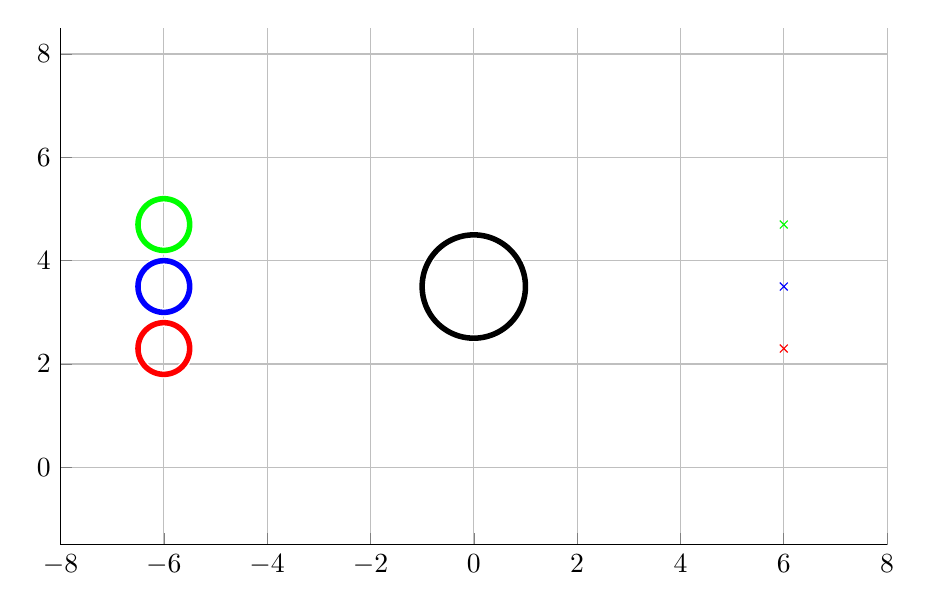
\begin{tikzpicture}

\begin{axis}[%
width=4.133in,
height=2.583in,
at={(0.693in,0.778in)},
scale only axis,
unbounded coords=jump,
xmin=-8,
xmax=8,
xmajorgrids,
ymin=-1.5,
ymax=8.5,
ymajorgrids,
axis background/.style={fill=white},
axis x line*=bottom,
axis y line*=left
]
\addplot [color=blue,only marks,mark=x,mark options={solid},forget plot]
  table[row sep=crcr]{%
6	3.5\\
};
\addplot [color=red,only marks,mark=x,mark options={solid},forget plot]
  table[row sep=crcr]{%
6	2.3\\
};
\addplot [color=green,only marks,mark=x,mark options={solid},forget plot]
  table[row sep=crcr]{%
6	4.7\\
};
\addplot [color=white,solid,line width=3.0pt,forget plot]
  table[row sep=crcr]{%
-5.5	3.5\\
-5.50030458649045	3.51744974835125\\
-5.50121797487009	3.53487823687206\\
-5.50273905231586	3.55226423163383\\
-5.50486596562921	3.56958655048003\\
-5.5075961234939	3.58682408883347\\
-5.5109261996331	3.60395584540888\\
-5.514852136862	3.62096094779983\\
-5.51936915203084	3.6378186779085\\
-5.52447174185242	3.65450849718747\\
-5.53015368960705	3.67101007166283\\
-5.53640807271661	3.68730329670796\\
-5.5432272711787	3.7033683215379\\
-5.55060297685042	3.71918557339454\\
-5.55852620357054	3.73473578139295\\
-5.56698729810778	3.75\\
-5.57597595192179	3.7649596321166\\
-5.58548121372248	3.77959645173537\\
-5.59549150281253	3.79389262614624\\
-5.60599462319664	3.80783073766283\\
-5.61697777844051	3.82139380484327\\
-5.6284275872613	3.83456530317943\\
-5.64033009983067	3.8473291852295\\
-5.6526708147705	3.85966990016933\\
-5.66543469682057	3.8715724127387\\
-5.67860619515673	3.88302222155949\\
-5.69216926233717	3.89400537680336\\
-5.70610737385376	3.90450849718747\\
-5.72040354826463	3.91451878627752\\
-5.7350403678834	3.92402404807821\\
-5.75	3.93301270189222\\
-5.76526421860705	3.94147379642946\\
-5.78081442660546	3.94939702314958\\
-5.7966316784621	3.9567727288213\\
-5.81269670329204	3.96359192728339\\
-5.82898992833717	3.96984631039295\\
-5.84549150281253	3.97552825814758\\
-5.8621813220915	3.98063084796916\\
-5.87903905220017	3.985147863138\\
-5.89604415459112	3.9890738003669\\
-5.91317591116653	3.9924038765061\\
-5.93041344951997	3.99513403437079\\
-5.94773576836617	3.99726094768414\\
-5.96512176312794	3.99878202512991\\
-5.98255025164875	3.99969541350955\\
-6	4\\
-6.01744974835125	3.99969541350955\\
-6.03487823687206	3.99878202512991\\
-6.05226423163383	3.99726094768414\\
-6.06958655048003	3.99513403437079\\
-6.08682408883347	3.9924038765061\\
-6.10395584540888	3.9890738003669\\
-6.12096094779983	3.985147863138\\
-6.1378186779085	3.98063084796916\\
-6.15450849718747	3.97552825814758\\
-6.17101007166283	3.96984631039295\\
-6.18730329670796	3.96359192728339\\
-6.2033683215379	3.9567727288213\\
-6.21918557339454	3.94939702314958\\
-6.23473578139295	3.94147379642946\\
-6.25	3.93301270189222\\
-6.2649596321166	3.92402404807821\\
-6.27959645173537	3.91451878627752\\
-6.29389262614624	3.90450849718747\\
-6.30783073766283	3.89400537680336\\
-6.32139380484327	3.88302222155949\\
-6.33456530317943	3.8715724127387\\
-6.3473291852295	3.85966990016933\\
-6.35966990016933	3.8473291852295\\
-6.3715724127387	3.83456530317943\\
-6.38302222155949	3.82139380484327\\
-6.39400537680336	3.80783073766283\\
-6.40450849718747	3.79389262614624\\
-6.41451878627752	3.77959645173537\\
-6.42402404807821	3.7649596321166\\
-6.43301270189222	3.75\\
-6.44147379642946	3.73473578139295\\
-6.44939702314958	3.71918557339454\\
-6.4567727288213	3.7033683215379\\
-6.46359192728339	3.68730329670796\\
-6.46984631039295	3.67101007166283\\
-6.47552825814758	3.65450849718747\\
-6.48063084796916	3.6378186779085\\
-6.485147863138	3.62096094779983\\
-6.4890738003669	3.60395584540888\\
-6.4924038765061	3.58682408883347\\
-6.49513403437079	3.56958655048003\\
-6.49726094768414	3.55226423163383\\
-6.49878202512991	3.53487823687206\\
-6.49969541350955	3.51744974835125\\
-6.5	3.5\\
-6.49969541350955	3.48255025164875\\
-6.49878202512991	3.46512176312794\\
-6.49726094768414	3.44773576836617\\
-6.49513403437079	3.43041344951997\\
-6.4924038765061	3.41317591116653\\
-6.4890738003669	3.39604415459112\\
-6.485147863138	3.37903905220017\\
-6.48063084796916	3.3621813220915\\
-6.47552825814758	3.34549150281253\\
-6.46984631039295	3.32898992833717\\
-6.46359192728339	3.31269670329204\\
-6.4567727288213	3.2966316784621\\
-6.44939702314958	3.28081442660546\\
-6.44147379642946	3.26526421860705\\
-6.43301270189222	3.25\\
-6.42402404807821	3.2350403678834\\
-6.41451878627752	3.22040354826463\\
-6.40450849718747	3.20610737385376\\
-6.39400537680336	3.19216926233717\\
-6.38302222155949	3.17860619515673\\
-6.3715724127387	3.16543469682057\\
-6.35966990016933	3.1526708147705\\
-6.3473291852295	3.14033009983067\\
-6.33456530317943	3.1284275872613\\
-6.32139380484327	3.11697777844051\\
-6.30783073766283	3.10599462319664\\
-6.29389262614624	3.09549150281253\\
-6.27959645173537	3.08548121372248\\
-6.2649596321166	3.07597595192179\\
-6.25	3.06698729810778\\
-6.23473578139295	3.05852620357054\\
-6.21918557339454	3.05060297685042\\
-6.2033683215379	3.0432272711787\\
-6.18730329670796	3.03640807271661\\
-6.17101007166283	3.03015368960705\\
-6.15450849718747	3.02447174185242\\
-6.1378186779085	3.01936915203084\\
-6.12096094779983	3.014852136862\\
-6.10395584540888	3.0109261996331\\
-6.08682408883347	3.0075961234939\\
-6.06958655048003	3.00486596562921\\
-6.05226423163383	3.00273905231586\\
-6.03487823687206	3.00121797487009\\
-6.01744974835125	3.00030458649045\\
-6	3\\
-5.98255025164875	3.00030458649045\\
-5.96512176312794	3.00121797487009\\
-5.94773576836617	3.00273905231586\\
-5.93041344951997	3.00486596562921\\
-5.91317591116653	3.0075961234939\\
-5.89604415459112	3.0109261996331\\
-5.87903905220017	3.014852136862\\
-5.8621813220915	3.01936915203084\\
-5.84549150281253	3.02447174185242\\
-5.82898992833717	3.03015368960705\\
-5.81269670329204	3.03640807271661\\
-5.7966316784621	3.0432272711787\\
-5.78081442660546	3.05060297685042\\
-5.76526421860705	3.05852620357054\\
-5.75	3.06698729810778\\
-5.7350403678834	3.07597595192179\\
-5.72040354826463	3.08548121372248\\
-5.70610737385376	3.09549150281253\\
-5.69216926233717	3.10599462319664\\
-5.67860619515673	3.11697777844051\\
-5.66543469682057	3.1284275872613\\
-5.6526708147705	3.14033009983067\\
-5.64033009983067	3.1526708147705\\
-5.6284275872613	3.16543469682057\\
-5.61697777844051	3.17860619515673\\
-5.60599462319664	3.19216926233717\\
-5.59549150281253	3.20610737385376\\
-5.58548121372248	3.22040354826463\\
-5.57597595192179	3.2350403678834\\
-5.56698729810778	3.25\\
-5.55852620357054	3.26526421860705\\
-5.55060297685042	3.28081442660546\\
-5.5432272711787	3.2966316784621\\
-5.53640807271661	3.31269670329204\\
-5.53015368960705	3.32898992833717\\
-5.52447174185242	3.34549150281253\\
-5.51936915203084	3.3621813220915\\
-5.514852136862	3.37903905220017\\
-5.5109261996331	3.39604415459112\\
-5.5075961234939	3.41317591116653\\
-5.50486596562921	3.43041344951997\\
-5.50273905231586	3.44773576836617\\
-5.50121797487009	3.46512176312794\\
-5.50030458649045	3.48255025164875\\
-5.5	3.5\\
nan	nan\\
};
\addplot [color=blue,solid,line width=2.0pt,forget plot]
  table[row sep=crcr]{%
-5.5	3.5\\
-5.50030458649045	3.51744974835125\\
-5.50121797487009	3.53487823687206\\
-5.50273905231586	3.55226423163383\\
-5.50486596562921	3.56958655048003\\
-5.5075961234939	3.58682408883347\\
-5.5109261996331	3.60395584540888\\
-5.514852136862	3.62096094779983\\
-5.51936915203084	3.6378186779085\\
-5.52447174185242	3.65450849718747\\
-5.53015368960705	3.67101007166283\\
-5.53640807271661	3.68730329670796\\
-5.5432272711787	3.7033683215379\\
-5.55060297685042	3.71918557339454\\
-5.55852620357054	3.73473578139295\\
-5.56698729810778	3.75\\
-5.57597595192179	3.7649596321166\\
-5.58548121372248	3.77959645173537\\
-5.59549150281253	3.79389262614624\\
-5.60599462319664	3.80783073766283\\
-5.61697777844051	3.82139380484327\\
-5.6284275872613	3.83456530317943\\
-5.64033009983067	3.8473291852295\\
-5.6526708147705	3.85966990016933\\
-5.66543469682057	3.8715724127387\\
-5.67860619515673	3.88302222155949\\
-5.69216926233717	3.89400537680336\\
-5.70610737385376	3.90450849718747\\
-5.72040354826463	3.91451878627752\\
-5.7350403678834	3.92402404807821\\
-5.75	3.93301270189222\\
-5.76526421860705	3.94147379642946\\
-5.78081442660546	3.94939702314958\\
-5.7966316784621	3.9567727288213\\
-5.81269670329204	3.96359192728339\\
-5.82898992833717	3.96984631039295\\
-5.84549150281253	3.97552825814758\\
-5.8621813220915	3.98063084796916\\
-5.87903905220017	3.985147863138\\
-5.89604415459112	3.9890738003669\\
-5.91317591116653	3.9924038765061\\
-5.93041344951997	3.99513403437079\\
-5.94773576836617	3.99726094768414\\
-5.96512176312794	3.99878202512991\\
-5.98255025164875	3.99969541350955\\
-6	4\\
-6.01744974835125	3.99969541350955\\
-6.03487823687206	3.99878202512991\\
-6.05226423163383	3.99726094768414\\
-6.06958655048003	3.99513403437079\\
-6.08682408883347	3.9924038765061\\
-6.10395584540888	3.9890738003669\\
-6.12096094779983	3.985147863138\\
-6.1378186779085	3.98063084796916\\
-6.15450849718747	3.97552825814758\\
-6.17101007166283	3.96984631039295\\
-6.18730329670796	3.96359192728339\\
-6.2033683215379	3.9567727288213\\
-6.21918557339454	3.94939702314958\\
-6.23473578139295	3.94147379642946\\
-6.25	3.93301270189222\\
-6.2649596321166	3.92402404807821\\
-6.27959645173537	3.91451878627752\\
-6.29389262614624	3.90450849718747\\
-6.30783073766283	3.89400537680336\\
-6.32139380484327	3.88302222155949\\
-6.33456530317943	3.8715724127387\\
-6.3473291852295	3.85966990016933\\
-6.35966990016933	3.8473291852295\\
-6.3715724127387	3.83456530317943\\
-6.38302222155949	3.82139380484327\\
-6.39400537680336	3.80783073766283\\
-6.40450849718747	3.79389262614624\\
-6.41451878627752	3.77959645173537\\
-6.42402404807821	3.7649596321166\\
-6.43301270189222	3.75\\
-6.44147379642946	3.73473578139295\\
-6.44939702314958	3.71918557339454\\
-6.4567727288213	3.7033683215379\\
-6.46359192728339	3.68730329670796\\
-6.46984631039295	3.67101007166283\\
-6.47552825814758	3.65450849718747\\
-6.48063084796916	3.6378186779085\\
-6.485147863138	3.62096094779983\\
-6.4890738003669	3.60395584540888\\
-6.4924038765061	3.58682408883347\\
-6.49513403437079	3.56958655048003\\
-6.49726094768414	3.55226423163383\\
-6.49878202512991	3.53487823687206\\
-6.49969541350955	3.51744974835125\\
-6.5	3.5\\
-6.49969541350955	3.48255025164875\\
-6.49878202512991	3.46512176312794\\
-6.49726094768414	3.44773576836617\\
-6.49513403437079	3.43041344951997\\
-6.4924038765061	3.41317591116653\\
-6.4890738003669	3.39604415459112\\
-6.485147863138	3.37903905220017\\
-6.48063084796916	3.3621813220915\\
-6.47552825814758	3.34549150281253\\
-6.46984631039295	3.32898992833717\\
-6.46359192728339	3.31269670329204\\
-6.4567727288213	3.2966316784621\\
-6.44939702314958	3.28081442660546\\
-6.44147379642946	3.26526421860705\\
-6.43301270189222	3.25\\
-6.42402404807821	3.2350403678834\\
-6.41451878627752	3.22040354826463\\
-6.40450849718747	3.20610737385376\\
-6.39400537680336	3.19216926233717\\
-6.38302222155949	3.17860619515673\\
-6.3715724127387	3.16543469682057\\
-6.35966990016933	3.1526708147705\\
-6.3473291852295	3.14033009983067\\
-6.33456530317943	3.1284275872613\\
-6.32139380484327	3.11697777844051\\
-6.30783073766283	3.10599462319664\\
-6.29389262614624	3.09549150281253\\
-6.27959645173537	3.08548121372248\\
-6.2649596321166	3.07597595192179\\
-6.25	3.06698729810778\\
-6.23473578139295	3.05852620357054\\
-6.21918557339454	3.05060297685042\\
-6.2033683215379	3.0432272711787\\
-6.18730329670796	3.03640807271661\\
-6.17101007166283	3.03015368960705\\
-6.15450849718747	3.02447174185242\\
-6.1378186779085	3.01936915203084\\
-6.12096094779983	3.014852136862\\
-6.10395584540888	3.0109261996331\\
-6.08682408883347	3.0075961234939\\
-6.06958655048003	3.00486596562921\\
-6.05226423163383	3.00273905231586\\
-6.03487823687206	3.00121797487009\\
-6.01744974835125	3.00030458649045\\
-6	3\\
-5.98255025164875	3.00030458649045\\
-5.96512176312794	3.00121797487009\\
-5.94773576836617	3.00273905231586\\
-5.93041344951997	3.00486596562921\\
-5.91317591116653	3.0075961234939\\
-5.89604415459112	3.0109261996331\\
-5.87903905220017	3.014852136862\\
-5.8621813220915	3.01936915203084\\
-5.84549150281253	3.02447174185242\\
-5.82898992833717	3.03015368960705\\
-5.81269670329204	3.03640807271661\\
-5.7966316784621	3.0432272711787\\
-5.78081442660546	3.05060297685042\\
-5.76526421860705	3.05852620357054\\
-5.75	3.06698729810778\\
-5.7350403678834	3.07597595192179\\
-5.72040354826463	3.08548121372248\\
-5.70610737385376	3.09549150281253\\
-5.69216926233717	3.10599462319664\\
-5.67860619515673	3.11697777844051\\
-5.66543469682057	3.1284275872613\\
-5.6526708147705	3.14033009983067\\
-5.64033009983067	3.1526708147705\\
-5.6284275872613	3.16543469682057\\
-5.61697777844051	3.17860619515673\\
-5.60599462319664	3.19216926233717\\
-5.59549150281253	3.20610737385376\\
-5.58548121372248	3.22040354826463\\
-5.57597595192179	3.2350403678834\\
-5.56698729810778	3.25\\
-5.55852620357054	3.26526421860705\\
-5.55060297685042	3.28081442660546\\
-5.5432272711787	3.2966316784621\\
-5.53640807271661	3.31269670329204\\
-5.53015368960705	3.32898992833717\\
-5.52447174185242	3.34549150281253\\
-5.51936915203084	3.3621813220915\\
-5.514852136862	3.37903905220017\\
-5.5109261996331	3.39604415459112\\
-5.5075961234939	3.41317591116653\\
-5.50486596562921	3.43041344951997\\
-5.50273905231586	3.44773576836617\\
-5.50121797487009	3.46512176312794\\
-5.50030458649045	3.48255025164875\\
-5.5	3.5\\
nan	nan\\
};
\addplot [color=white,solid,line width=3.0pt,forget plot]
  table[row sep=crcr]{%
-5.5	2.3\\
-5.50030458649045	2.31744974835125\\
-5.50121797487009	2.33487823687206\\
-5.50273905231586	2.35226423163383\\
-5.50486596562921	2.36958655048003\\
-5.5075961234939	2.38682408883346\\
-5.5109261996331	2.40395584540888\\
-5.514852136862	2.42096094779983\\
-5.51936915203084	2.4378186779085\\
-5.52447174185242	2.45450849718747\\
-5.53015368960705	2.47101007166283\\
-5.53640807271661	2.48730329670796\\
-5.5432272711787	2.5033683215379\\
-5.55060297685042	2.51918557339454\\
-5.55852620357054	2.53473578139295\\
-5.56698729810778	2.55\\
-5.57597595192179	2.5649596321166\\
-5.58548121372248	2.57959645173537\\
-5.59549150281253	2.59389262614624\\
-5.60599462319664	2.60783073766283\\
-5.61697777844051	2.62139380484327\\
-5.6284275872613	2.63456530317943\\
-5.64033009983067	2.6473291852295\\
-5.6526708147705	2.65966990016933\\
-5.66543469682057	2.6715724127387\\
-5.67860619515673	2.68302222155949\\
-5.69216926233717	2.69400537680336\\
-5.70610737385376	2.70450849718747\\
-5.72040354826463	2.71451878627752\\
-5.7350403678834	2.72402404807821\\
-5.75	2.73301270189222\\
-5.76526421860705	2.74147379642946\\
-5.78081442660546	2.74939702314958\\
-5.7966316784621	2.7567727288213\\
-5.81269670329204	2.76359192728339\\
-5.82898992833717	2.76984631039295\\
-5.84549150281253	2.77552825814758\\
-5.8621813220915	2.78063084796916\\
-5.87903905220017	2.785147863138\\
-5.89604415459112	2.7890738003669\\
-5.91317591116653	2.7924038765061\\
-5.93041344951997	2.79513403437078\\
-5.94773576836617	2.79726094768414\\
-5.96512176312794	2.79878202512991\\
-5.98255025164875	2.79969541350955\\
-6	2.8\\
-6.01744974835125	2.79969541350955\\
-6.03487823687206	2.79878202512991\\
-6.05226423163383	2.79726094768414\\
-6.06958655048003	2.79513403437078\\
-6.08682408883347	2.7924038765061\\
-6.10395584540888	2.7890738003669\\
-6.12096094779983	2.785147863138\\
-6.1378186779085	2.78063084796916\\
-6.15450849718747	2.77552825814758\\
-6.17101007166283	2.76984631039295\\
-6.18730329670796	2.76359192728339\\
-6.2033683215379	2.7567727288213\\
-6.21918557339454	2.74939702314958\\
-6.23473578139295	2.74147379642946\\
-6.25	2.73301270189222\\
-6.2649596321166	2.72402404807821\\
-6.27959645173537	2.71451878627752\\
-6.29389262614624	2.70450849718747\\
-6.30783073766283	2.69400537680336\\
-6.32139380484327	2.68302222155949\\
-6.33456530317943	2.6715724127387\\
-6.3473291852295	2.65966990016933\\
-6.35966990016933	2.6473291852295\\
-6.3715724127387	2.63456530317943\\
-6.38302222155949	2.62139380484327\\
-6.39400537680336	2.60783073766283\\
-6.40450849718747	2.59389262614624\\
-6.41451878627752	2.57959645173537\\
-6.42402404807821	2.5649596321166\\
-6.43301270189222	2.55\\
-6.44147379642946	2.53473578139295\\
-6.44939702314958	2.51918557339454\\
-6.4567727288213	2.5033683215379\\
-6.46359192728339	2.48730329670796\\
-6.46984631039295	2.47101007166283\\
-6.47552825814758	2.45450849718747\\
-6.48063084796916	2.4378186779085\\
-6.485147863138	2.42096094779983\\
-6.4890738003669	2.40395584540888\\
-6.4924038765061	2.38682408883346\\
-6.49513403437079	2.36958655048003\\
-6.49726094768414	2.35226423163383\\
-6.49878202512991	2.33487823687206\\
-6.49969541350955	2.31744974835125\\
-6.5	2.3\\
-6.49969541350955	2.28255025164875\\
-6.49878202512991	2.26512176312794\\
-6.49726094768414	2.24773576836617\\
-6.49513403437079	2.23041344951997\\
-6.4924038765061	2.21317591116653\\
-6.4890738003669	2.19604415459112\\
-6.485147863138	2.17903905220017\\
-6.48063084796916	2.1621813220915\\
-6.47552825814758	2.14549150281253\\
-6.46984631039295	2.12898992833717\\
-6.46359192728339	2.11269670329204\\
-6.4567727288213	2.0966316784621\\
-6.44939702314958	2.08081442660546\\
-6.44147379642946	2.06526421860705\\
-6.43301270189222	2.05\\
-6.42402404807821	2.0350403678834\\
-6.41451878627752	2.02040354826463\\
-6.40450849718747	2.00610737385376\\
-6.39400537680336	1.99216926233717\\
-6.38302222155949	1.97860619515673\\
-6.3715724127387	1.96543469682057\\
-6.35966990016933	1.9526708147705\\
-6.3473291852295	1.94033009983067\\
-6.33456530317943	1.9284275872613\\
-6.32139380484327	1.91697777844051\\
-6.30783073766283	1.90599462319664\\
-6.29389262614624	1.89549150281253\\
-6.27959645173537	1.88548121372248\\
-6.2649596321166	1.87597595192179\\
-6.25	1.86698729810778\\
-6.23473578139295	1.85852620357054\\
-6.21918557339454	1.85060297685042\\
-6.2033683215379	1.8432272711787\\
-6.18730329670796	1.83640807271661\\
-6.17101007166283	1.83015368960705\\
-6.15450849718747	1.82447174185242\\
-6.1378186779085	1.81936915203084\\
-6.12096094779983	1.814852136862\\
-6.10395584540888	1.8109261996331\\
-6.08682408883347	1.8075961234939\\
-6.06958655048003	1.80486596562921\\
-6.05226423163383	1.80273905231586\\
-6.03487823687206	1.80121797487009\\
-6.01744974835125	1.80030458649045\\
-6	1.8\\
-5.98255025164875	1.80030458649045\\
-5.96512176312794	1.80121797487009\\
-5.94773576836617	1.80273905231586\\
-5.93041344951997	1.80486596562921\\
-5.91317591116653	1.8075961234939\\
-5.89604415459112	1.8109261996331\\
-5.87903905220017	1.814852136862\\
-5.8621813220915	1.81936915203084\\
-5.84549150281253	1.82447174185242\\
-5.82898992833717	1.83015368960705\\
-5.81269670329204	1.83640807271661\\
-5.7966316784621	1.8432272711787\\
-5.78081442660546	1.85060297685042\\
-5.76526421860705	1.85852620357054\\
-5.75	1.86698729810778\\
-5.7350403678834	1.87597595192179\\
-5.72040354826463	1.88548121372248\\
-5.70610737385376	1.89549150281253\\
-5.69216926233717	1.90599462319664\\
-5.67860619515673	1.91697777844051\\
-5.66543469682057	1.9284275872613\\
-5.6526708147705	1.94033009983067\\
-5.64033009983067	1.9526708147705\\
-5.6284275872613	1.96543469682057\\
-5.61697777844051	1.97860619515673\\
-5.60599462319664	1.99216926233717\\
-5.59549150281253	2.00610737385376\\
-5.58548121372248	2.02040354826463\\
-5.57597595192179	2.0350403678834\\
-5.56698729810778	2.05\\
-5.55852620357054	2.06526421860705\\
-5.55060297685042	2.08081442660546\\
-5.5432272711787	2.0966316784621\\
-5.53640807271661	2.11269670329204\\
-5.53015368960705	2.12898992833717\\
-5.52447174185242	2.14549150281253\\
-5.51936915203084	2.1621813220915\\
-5.514852136862	2.17903905220017\\
-5.5109261996331	2.19604415459112\\
-5.5075961234939	2.21317591116653\\
-5.50486596562921	2.23041344951997\\
-5.50273905231586	2.24773576836617\\
-5.50121797487009	2.26512176312794\\
-5.50030458649045	2.28255025164875\\
-5.5	2.3\\
nan	nan\\
};
\addplot [color=red,solid,line width=2.0pt,forget plot]
  table[row sep=crcr]{%
-5.5	2.3\\
-5.50030458649045	2.31744974835125\\
-5.50121797487009	2.33487823687206\\
-5.50273905231586	2.35226423163383\\
-5.50486596562921	2.36958655048003\\
-5.5075961234939	2.38682408883346\\
-5.5109261996331	2.40395584540888\\
-5.514852136862	2.42096094779983\\
-5.51936915203084	2.4378186779085\\
-5.52447174185242	2.45450849718747\\
-5.53015368960705	2.47101007166283\\
-5.53640807271661	2.48730329670796\\
-5.5432272711787	2.5033683215379\\
-5.55060297685042	2.51918557339454\\
-5.55852620357054	2.53473578139295\\
-5.56698729810778	2.55\\
-5.57597595192179	2.5649596321166\\
-5.58548121372248	2.57959645173537\\
-5.59549150281253	2.59389262614624\\
-5.60599462319664	2.60783073766283\\
-5.61697777844051	2.62139380484327\\
-5.6284275872613	2.63456530317943\\
-5.64033009983067	2.6473291852295\\
-5.6526708147705	2.65966990016933\\
-5.66543469682057	2.6715724127387\\
-5.67860619515673	2.68302222155949\\
-5.69216926233717	2.69400537680336\\
-5.70610737385376	2.70450849718747\\
-5.72040354826463	2.71451878627752\\
-5.7350403678834	2.72402404807821\\
-5.75	2.73301270189222\\
-5.76526421860705	2.74147379642946\\
-5.78081442660546	2.74939702314958\\
-5.7966316784621	2.7567727288213\\
-5.81269670329204	2.76359192728339\\
-5.82898992833717	2.76984631039295\\
-5.84549150281253	2.77552825814758\\
-5.8621813220915	2.78063084796916\\
-5.87903905220017	2.785147863138\\
-5.89604415459112	2.7890738003669\\
-5.91317591116653	2.7924038765061\\
-5.93041344951997	2.79513403437078\\
-5.94773576836617	2.79726094768414\\
-5.96512176312794	2.79878202512991\\
-5.98255025164875	2.79969541350955\\
-6	2.8\\
-6.01744974835125	2.79969541350955\\
-6.03487823687206	2.79878202512991\\
-6.05226423163383	2.79726094768414\\
-6.06958655048003	2.79513403437078\\
-6.08682408883347	2.7924038765061\\
-6.10395584540888	2.7890738003669\\
-6.12096094779983	2.785147863138\\
-6.1378186779085	2.78063084796916\\
-6.15450849718747	2.77552825814758\\
-6.17101007166283	2.76984631039295\\
-6.18730329670796	2.76359192728339\\
-6.2033683215379	2.7567727288213\\
-6.21918557339454	2.74939702314958\\
-6.23473578139295	2.74147379642946\\
-6.25	2.73301270189222\\
-6.2649596321166	2.72402404807821\\
-6.27959645173537	2.71451878627752\\
-6.29389262614624	2.70450849718747\\
-6.30783073766283	2.69400537680336\\
-6.32139380484327	2.68302222155949\\
-6.33456530317943	2.6715724127387\\
-6.3473291852295	2.65966990016933\\
-6.35966990016933	2.6473291852295\\
-6.3715724127387	2.63456530317943\\
-6.38302222155949	2.62139380484327\\
-6.39400537680336	2.60783073766283\\
-6.40450849718747	2.59389262614624\\
-6.41451878627752	2.57959645173537\\
-6.42402404807821	2.5649596321166\\
-6.43301270189222	2.55\\
-6.44147379642946	2.53473578139295\\
-6.44939702314958	2.51918557339454\\
-6.4567727288213	2.5033683215379\\
-6.46359192728339	2.48730329670796\\
-6.46984631039295	2.47101007166283\\
-6.47552825814758	2.45450849718747\\
-6.48063084796916	2.4378186779085\\
-6.485147863138	2.42096094779983\\
-6.4890738003669	2.40395584540888\\
-6.4924038765061	2.38682408883346\\
-6.49513403437079	2.36958655048003\\
-6.49726094768414	2.35226423163383\\
-6.49878202512991	2.33487823687206\\
-6.49969541350955	2.31744974835125\\
-6.5	2.3\\
-6.49969541350955	2.28255025164875\\
-6.49878202512991	2.26512176312794\\
-6.49726094768414	2.24773576836617\\
-6.49513403437079	2.23041344951997\\
-6.4924038765061	2.21317591116653\\
-6.4890738003669	2.19604415459112\\
-6.485147863138	2.17903905220017\\
-6.48063084796916	2.1621813220915\\
-6.47552825814758	2.14549150281253\\
-6.46984631039295	2.12898992833717\\
-6.46359192728339	2.11269670329204\\
-6.4567727288213	2.0966316784621\\
-6.44939702314958	2.08081442660546\\
-6.44147379642946	2.06526421860705\\
-6.43301270189222	2.05\\
-6.42402404807821	2.0350403678834\\
-6.41451878627752	2.02040354826463\\
-6.40450849718747	2.00610737385376\\
-6.39400537680336	1.99216926233717\\
-6.38302222155949	1.97860619515673\\
-6.3715724127387	1.96543469682057\\
-6.35966990016933	1.9526708147705\\
-6.3473291852295	1.94033009983067\\
-6.33456530317943	1.9284275872613\\
-6.32139380484327	1.91697777844051\\
-6.30783073766283	1.90599462319664\\
-6.29389262614624	1.89549150281253\\
-6.27959645173537	1.88548121372248\\
-6.2649596321166	1.87597595192179\\
-6.25	1.86698729810778\\
-6.23473578139295	1.85852620357054\\
-6.21918557339454	1.85060297685042\\
-6.2033683215379	1.8432272711787\\
-6.18730329670796	1.83640807271661\\
-6.17101007166283	1.83015368960705\\
-6.15450849718747	1.82447174185242\\
-6.1378186779085	1.81936915203084\\
-6.12096094779983	1.814852136862\\
-6.10395584540888	1.8109261996331\\
-6.08682408883347	1.8075961234939\\
-6.06958655048003	1.80486596562921\\
-6.05226423163383	1.80273905231586\\
-6.03487823687206	1.80121797487009\\
-6.01744974835125	1.80030458649045\\
-6	1.8\\
-5.98255025164875	1.80030458649045\\
-5.96512176312794	1.80121797487009\\
-5.94773576836617	1.80273905231586\\
-5.93041344951997	1.80486596562921\\
-5.91317591116653	1.8075961234939\\
-5.89604415459112	1.8109261996331\\
-5.87903905220017	1.814852136862\\
-5.8621813220915	1.81936915203084\\
-5.84549150281253	1.82447174185242\\
-5.82898992833717	1.83015368960705\\
-5.81269670329204	1.83640807271661\\
-5.7966316784621	1.8432272711787\\
-5.78081442660546	1.85060297685042\\
-5.76526421860705	1.85852620357054\\
-5.75	1.86698729810778\\
-5.7350403678834	1.87597595192179\\
-5.72040354826463	1.88548121372248\\
-5.70610737385376	1.89549150281253\\
-5.69216926233717	1.90599462319664\\
-5.67860619515673	1.91697777844051\\
-5.66543469682057	1.9284275872613\\
-5.6526708147705	1.94033009983067\\
-5.64033009983067	1.9526708147705\\
-5.6284275872613	1.96543469682057\\
-5.61697777844051	1.97860619515673\\
-5.60599462319664	1.99216926233717\\
-5.59549150281253	2.00610737385376\\
-5.58548121372248	2.02040354826463\\
-5.57597595192179	2.0350403678834\\
-5.56698729810778	2.05\\
-5.55852620357054	2.06526421860705\\
-5.55060297685042	2.08081442660546\\
-5.5432272711787	2.0966316784621\\
-5.53640807271661	2.11269670329204\\
-5.53015368960705	2.12898992833717\\
-5.52447174185242	2.14549150281253\\
-5.51936915203084	2.1621813220915\\
-5.514852136862	2.17903905220017\\
-5.5109261996331	2.19604415459112\\
-5.5075961234939	2.21317591116653\\
-5.50486596562921	2.23041344951997\\
-5.50273905231586	2.24773576836617\\
-5.50121797487009	2.26512176312794\\
-5.50030458649045	2.28255025164875\\
-5.5	2.3\\
nan	nan\\
};
\addplot [color=white,solid,line width=3.0pt,forget plot]
  table[row sep=crcr]{%
-5.5	4.7\\
-5.50030458649045	4.71744974835125\\
-5.50121797487009	4.73487823687206\\
-5.50273905231586	4.75226423163383\\
-5.50486596562921	4.76958655048003\\
-5.5075961234939	4.78682408883347\\
-5.5109261996331	4.80395584540888\\
-5.514852136862	4.82096094779983\\
-5.51936915203084	4.8378186779085\\
-5.52447174185242	4.85450849718747\\
-5.53015368960705	4.87101007166283\\
-5.53640807271661	4.88730329670796\\
-5.5432272711787	4.9033683215379\\
-5.55060297685042	4.91918557339454\\
-5.55852620357054	4.93473578139295\\
-5.56698729810778	4.95\\
-5.57597595192179	4.9649596321166\\
-5.58548121372248	4.97959645173537\\
-5.59549150281253	4.99389262614624\\
-5.60599462319664	5.00783073766283\\
-5.61697777844051	5.02139380484327\\
-5.6284275872613	5.03456530317943\\
-5.64033009983067	5.0473291852295\\
-5.6526708147705	5.05966990016933\\
-5.66543469682057	5.0715724127387\\
-5.67860619515673	5.08302222155949\\
-5.69216926233717	5.09400537680336\\
-5.70610737385376	5.10450849718747\\
-5.72040354826463	5.11451878627752\\
-5.7350403678834	5.12402404807821\\
-5.75	5.13301270189222\\
-5.76526421860705	5.14147379642946\\
-5.78081442660546	5.14939702314958\\
-5.7966316784621	5.1567727288213\\
-5.81269670329204	5.16359192728339\\
-5.82898992833717	5.16984631039295\\
-5.84549150281253	5.17552825814758\\
-5.8621813220915	5.18063084796916\\
-5.87903905220017	5.185147863138\\
-5.89604415459112	5.1890738003669\\
-5.91317591116653	5.1924038765061\\
-5.93041344951997	5.19513403437079\\
-5.94773576836617	5.19726094768414\\
-5.96512176312794	5.19878202512991\\
-5.98255025164875	5.19969541350955\\
-6	5.2\\
-6.01744974835125	5.19969541350955\\
-6.03487823687206	5.19878202512991\\
-6.05226423163383	5.19726094768414\\
-6.06958655048003	5.19513403437079\\
-6.08682408883347	5.1924038765061\\
-6.10395584540888	5.1890738003669\\
-6.12096094779983	5.185147863138\\
-6.1378186779085	5.18063084796916\\
-6.15450849718747	5.17552825814758\\
-6.17101007166283	5.16984631039295\\
-6.18730329670796	5.16359192728339\\
-6.2033683215379	5.1567727288213\\
-6.21918557339454	5.14939702314958\\
-6.23473578139295	5.14147379642946\\
-6.25	5.13301270189222\\
-6.2649596321166	5.12402404807821\\
-6.27959645173537	5.11451878627752\\
-6.29389262614624	5.10450849718747\\
-6.30783073766283	5.09400537680336\\
-6.32139380484327	5.08302222155949\\
-6.33456530317943	5.0715724127387\\
-6.3473291852295	5.05966990016933\\
-6.35966990016933	5.0473291852295\\
-6.3715724127387	5.03456530317943\\
-6.38302222155949	5.02139380484327\\
-6.39400537680336	5.00783073766283\\
-6.40450849718747	4.99389262614624\\
-6.41451878627752	4.97959645173537\\
-6.42402404807821	4.9649596321166\\
-6.43301270189222	4.95\\
-6.44147379642946	4.93473578139295\\
-6.44939702314958	4.91918557339454\\
-6.4567727288213	4.9033683215379\\
-6.46359192728339	4.88730329670796\\
-6.46984631039295	4.87101007166283\\
-6.47552825814758	4.85450849718747\\
-6.48063084796916	4.8378186779085\\
-6.485147863138	4.82096094779983\\
-6.4890738003669	4.80395584540888\\
-6.4924038765061	4.78682408883347\\
-6.49513403437079	4.76958655048003\\
-6.49726094768414	4.75226423163383\\
-6.49878202512991	4.73487823687206\\
-6.49969541350955	4.71744974835125\\
-6.5	4.7\\
-6.49969541350955	4.68255025164875\\
-6.49878202512991	4.66512176312794\\
-6.49726094768414	4.64773576836617\\
-6.49513403437079	4.63041344951997\\
-6.4924038765061	4.61317591116654\\
-6.4890738003669	4.59604415459112\\
-6.485147863138	4.57903905220017\\
-6.48063084796916	4.5621813220915\\
-6.47552825814758	4.54549150281253\\
-6.46984631039295	4.52898992833717\\
-6.46359192728339	4.51269670329204\\
-6.4567727288213	4.4966316784621\\
-6.44939702314958	4.48081442660546\\
-6.44147379642946	4.46526421860705\\
-6.43301270189222	4.45\\
-6.42402404807821	4.4350403678834\\
-6.41451878627752	4.42040354826463\\
-6.40450849718747	4.40610737385376\\
-6.39400537680336	4.39216926233717\\
-6.38302222155949	4.37860619515673\\
-6.3715724127387	4.36543469682057\\
-6.35966990016933	4.3526708147705\\
-6.3473291852295	4.34033009983068\\
-6.33456530317943	4.3284275872613\\
-6.32139380484327	4.31697777844051\\
-6.30783073766283	4.30599462319664\\
-6.29389262614624	4.29549150281253\\
-6.27959645173537	4.28548121372248\\
-6.2649596321166	4.27597595192179\\
-6.25	4.26698729810778\\
-6.23473578139295	4.25852620357054\\
-6.21918557339454	4.25060297685042\\
-6.2033683215379	4.2432272711787\\
-6.18730329670796	4.23640807271661\\
-6.17101007166283	4.23015368960705\\
-6.15450849718747	4.22447174185242\\
-6.1378186779085	4.21936915203084\\
-6.12096094779983	4.214852136862\\
-6.10395584540888	4.2109261996331\\
-6.08682408883347	4.2075961234939\\
-6.06958655048003	4.20486596562921\\
-6.05226423163383	4.20273905231586\\
-6.03487823687206	4.20121797487009\\
-6.01744974835125	4.20030458649045\\
-6	4.2\\
-5.98255025164875	4.20030458649045\\
-5.96512176312794	4.20121797487009\\
-5.94773576836617	4.20273905231586\\
-5.93041344951997	4.20486596562921\\
-5.91317591116653	4.2075961234939\\
-5.89604415459112	4.2109261996331\\
-5.87903905220017	4.214852136862\\
-5.8621813220915	4.21936915203084\\
-5.84549150281253	4.22447174185242\\
-5.82898992833717	4.23015368960705\\
-5.81269670329204	4.23640807271661\\
-5.7966316784621	4.2432272711787\\
-5.78081442660546	4.25060297685042\\
-5.76526421860705	4.25852620357054\\
-5.75	4.26698729810778\\
-5.7350403678834	4.27597595192179\\
-5.72040354826463	4.28548121372248\\
-5.70610737385376	4.29549150281253\\
-5.69216926233717	4.30599462319664\\
-5.67860619515673	4.31697777844051\\
-5.66543469682057	4.3284275872613\\
-5.6526708147705	4.34033009983067\\
-5.64033009983067	4.3526708147705\\
-5.6284275872613	4.36543469682057\\
-5.61697777844051	4.37860619515673\\
-5.60599462319664	4.39216926233717\\
-5.59549150281253	4.40610737385376\\
-5.58548121372248	4.42040354826463\\
-5.57597595192179	4.4350403678834\\
-5.56698729810778	4.45\\
-5.55852620357054	4.46526421860705\\
-5.55060297685042	4.48081442660546\\
-5.5432272711787	4.4966316784621\\
-5.53640807271661	4.51269670329204\\
-5.53015368960705	4.52898992833717\\
-5.52447174185242	4.54549150281253\\
-5.51936915203084	4.5621813220915\\
-5.514852136862	4.57903905220017\\
-5.5109261996331	4.59604415459112\\
-5.5075961234939	4.61317591116653\\
-5.50486596562921	4.63041344951997\\
-5.50273905231586	4.64773576836617\\
-5.50121797487009	4.66512176312794\\
-5.50030458649045	4.68255025164875\\
-5.5	4.7\\
nan	nan\\
};
\addplot [color=green,solid,line width=2.0pt,forget plot]
  table[row sep=crcr]{%
-5.5	4.7\\
-5.50030458649045	4.71744974835125\\
-5.50121797487009	4.73487823687206\\
-5.50273905231586	4.75226423163383\\
-5.50486596562921	4.76958655048003\\
-5.5075961234939	4.78682408883347\\
-5.5109261996331	4.80395584540888\\
-5.514852136862	4.82096094779983\\
-5.51936915203084	4.8378186779085\\
-5.52447174185242	4.85450849718747\\
-5.53015368960705	4.87101007166283\\
-5.53640807271661	4.88730329670796\\
-5.5432272711787	4.9033683215379\\
-5.55060297685042	4.91918557339454\\
-5.55852620357054	4.93473578139295\\
-5.56698729810778	4.95\\
-5.57597595192179	4.9649596321166\\
-5.58548121372248	4.97959645173537\\
-5.59549150281253	4.99389262614624\\
-5.60599462319664	5.00783073766283\\
-5.61697777844051	5.02139380484327\\
-5.6284275872613	5.03456530317943\\
-5.64033009983067	5.0473291852295\\
-5.6526708147705	5.05966990016933\\
-5.66543469682057	5.0715724127387\\
-5.67860619515673	5.08302222155949\\
-5.69216926233717	5.09400537680336\\
-5.70610737385376	5.10450849718747\\
-5.72040354826463	5.11451878627752\\
-5.7350403678834	5.12402404807821\\
-5.75	5.13301270189222\\
-5.76526421860705	5.14147379642946\\
-5.78081442660546	5.14939702314958\\
-5.7966316784621	5.1567727288213\\
-5.81269670329204	5.16359192728339\\
-5.82898992833717	5.16984631039295\\
-5.84549150281253	5.17552825814758\\
-5.8621813220915	5.18063084796916\\
-5.87903905220017	5.185147863138\\
-5.89604415459112	5.1890738003669\\
-5.91317591116653	5.1924038765061\\
-5.93041344951997	5.19513403437079\\
-5.94773576836617	5.19726094768414\\
-5.96512176312794	5.19878202512991\\
-5.98255025164875	5.19969541350955\\
-6	5.2\\
-6.01744974835125	5.19969541350955\\
-6.03487823687206	5.19878202512991\\
-6.05226423163383	5.19726094768414\\
-6.06958655048003	5.19513403437079\\
-6.08682408883347	5.1924038765061\\
-6.10395584540888	5.1890738003669\\
-6.12096094779983	5.185147863138\\
-6.1378186779085	5.18063084796916\\
-6.15450849718747	5.17552825814758\\
-6.17101007166283	5.16984631039295\\
-6.18730329670796	5.16359192728339\\
-6.2033683215379	5.1567727288213\\
-6.21918557339454	5.14939702314958\\
-6.23473578139295	5.14147379642946\\
-6.25	5.13301270189222\\
-6.2649596321166	5.12402404807821\\
-6.27959645173537	5.11451878627752\\
-6.29389262614624	5.10450849718747\\
-6.30783073766283	5.09400537680336\\
-6.32139380484327	5.08302222155949\\
-6.33456530317943	5.0715724127387\\
-6.3473291852295	5.05966990016933\\
-6.35966990016933	5.0473291852295\\
-6.3715724127387	5.03456530317943\\
-6.38302222155949	5.02139380484327\\
-6.39400537680336	5.00783073766283\\
-6.40450849718747	4.99389262614624\\
-6.41451878627752	4.97959645173537\\
-6.42402404807821	4.9649596321166\\
-6.43301270189222	4.95\\
-6.44147379642946	4.93473578139295\\
-6.44939702314958	4.91918557339454\\
-6.4567727288213	4.9033683215379\\
-6.46359192728339	4.88730329670796\\
-6.46984631039295	4.87101007166283\\
-6.47552825814758	4.85450849718747\\
-6.48063084796916	4.8378186779085\\
-6.485147863138	4.82096094779983\\
-6.4890738003669	4.80395584540888\\
-6.4924038765061	4.78682408883347\\
-6.49513403437079	4.76958655048003\\
-6.49726094768414	4.75226423163383\\
-6.49878202512991	4.73487823687206\\
-6.49969541350955	4.71744974835125\\
-6.5	4.7\\
-6.49969541350955	4.68255025164875\\
-6.49878202512991	4.66512176312794\\
-6.49726094768414	4.64773576836617\\
-6.49513403437079	4.63041344951997\\
-6.4924038765061	4.61317591116654\\
-6.4890738003669	4.59604415459112\\
-6.485147863138	4.57903905220017\\
-6.48063084796916	4.5621813220915\\
-6.47552825814758	4.54549150281253\\
-6.46984631039295	4.52898992833717\\
-6.46359192728339	4.51269670329204\\
-6.4567727288213	4.4966316784621\\
-6.44939702314958	4.48081442660546\\
-6.44147379642946	4.46526421860705\\
-6.43301270189222	4.45\\
-6.42402404807821	4.4350403678834\\
-6.41451878627752	4.42040354826463\\
-6.40450849718747	4.40610737385376\\
-6.39400537680336	4.39216926233717\\
-6.38302222155949	4.37860619515673\\
-6.3715724127387	4.36543469682057\\
-6.35966990016933	4.3526708147705\\
-6.3473291852295	4.34033009983068\\
-6.33456530317943	4.3284275872613\\
-6.32139380484327	4.31697777844051\\
-6.30783073766283	4.30599462319664\\
-6.29389262614624	4.29549150281253\\
-6.27959645173537	4.28548121372248\\
-6.2649596321166	4.27597595192179\\
-6.25	4.26698729810778\\
-6.23473578139295	4.25852620357054\\
-6.21918557339454	4.25060297685042\\
-6.2033683215379	4.2432272711787\\
-6.18730329670796	4.23640807271661\\
-6.17101007166283	4.23015368960705\\
-6.15450849718747	4.22447174185242\\
-6.1378186779085	4.21936915203084\\
-6.12096094779983	4.214852136862\\
-6.10395584540888	4.2109261996331\\
-6.08682408883347	4.2075961234939\\
-6.06958655048003	4.20486596562921\\
-6.05226423163383	4.20273905231586\\
-6.03487823687206	4.20121797487009\\
-6.01744974835125	4.20030458649045\\
-6	4.2\\
-5.98255025164875	4.20030458649045\\
-5.96512176312794	4.20121797487009\\
-5.94773576836617	4.20273905231586\\
-5.93041344951997	4.20486596562921\\
-5.91317591116653	4.2075961234939\\
-5.89604415459112	4.2109261996331\\
-5.87903905220017	4.214852136862\\
-5.8621813220915	4.21936915203084\\
-5.84549150281253	4.22447174185242\\
-5.82898992833717	4.23015368960705\\
-5.81269670329204	4.23640807271661\\
-5.7966316784621	4.2432272711787\\
-5.78081442660546	4.25060297685042\\
-5.76526421860705	4.25852620357054\\
-5.75	4.26698729810778\\
-5.7350403678834	4.27597595192179\\
-5.72040354826463	4.28548121372248\\
-5.70610737385376	4.29549150281253\\
-5.69216926233717	4.30599462319664\\
-5.67860619515673	4.31697777844051\\
-5.66543469682057	4.3284275872613\\
-5.6526708147705	4.34033009983067\\
-5.64033009983067	4.3526708147705\\
-5.6284275872613	4.36543469682057\\
-5.61697777844051	4.37860619515673\\
-5.60599462319664	4.39216926233717\\
-5.59549150281253	4.40610737385376\\
-5.58548121372248	4.42040354826463\\
-5.57597595192179	4.4350403678834\\
-5.56698729810778	4.45\\
-5.55852620357054	4.46526421860705\\
-5.55060297685042	4.48081442660546\\
-5.5432272711787	4.4966316784621\\
-5.53640807271661	4.51269670329204\\
-5.53015368960705	4.52898992833717\\
-5.52447174185242	4.54549150281253\\
-5.51936915203084	4.5621813220915\\
-5.514852136862	4.57903905220017\\
-5.5109261996331	4.59604415459112\\
-5.5075961234939	4.61317591116653\\
-5.50486596562921	4.63041344951997\\
-5.50273905231586	4.64773576836617\\
-5.50121797487009	4.66512176312794\\
-5.50030458649045	4.68255025164875\\
-5.5	4.7\\
nan	nan\\
};
\addplot [color=white,solid,line width=3.0pt,forget plot]
  table[row sep=crcr]{%
1	3.5\\
0.999390827019096	3.5348994967025\\
0.997564050259824	3.56975647374413\\
0.994521895368273	3.60452846326765\\
0.99026806874157	3.63917310096007\\
0.984807753012208	3.67364817766693\\
0.978147600733806	3.70791169081776\\
0.970295726275996	3.74192189559967\\
0.961261695938319	3.775637355817\\
0.951056516295154	3.80901699437495\\
0.939692620785908	3.84202014332567\\
0.927183854566787	3.87460659341591\\
0.913545457642601	3.9067366430758\\
0.898794046299167	3.93837114678908\\
0.882947592858927	3.96947156278589\\
0.866025403784439	4\\
0.848048096156426	4.0299192642332\\
0.829037572555042	4.05919290347075\\
0.809016994374947	4.08778525229247\\
0.788010753606722	4.11566147532566\\
0.766044443118978	4.14278760968654\\
0.743144825477394	4.16913060635886\\
0.719339800338651	4.194658370459\\
0.694658370458997	4.21933980033865\\
0.669130606358858	4.24314482547739\\
0.642787609686539	4.26604444311898\\
0.615661475325658	4.28801075360672\\
0.587785252292473	4.30901699437495\\
0.559192903470747	4.32903757255504\\
0.529919264233205	4.34804809615643\\
0.5	4.36602540378444\\
0.469471562785891	4.38294759285893\\
0.438371146789077	4.39879404629917\\
0.4067366430758	4.4135454576426\\
0.374606593415912	4.42718385456679\\
0.342020143325669	4.43969262078591\\
0.309016994374947	4.45105651629515\\
0.275637355816999	4.46126169593832\\
0.241921895599668	4.470295726276\\
0.207911690817759	4.47814760073381\\
0.17364817766693	4.48480775301221\\
0.139173100960066	4.49026806874157\\
0.104528463267653	4.49452189536827\\
0.0697564737441255	4.49756405025982\\
0.0348994967025011	4.4993908270191\\
6.12323399573677e-17	4.5\\
-0.0348994967025007	4.4993908270191\\
-0.0697564737441253	4.49756405025982\\
-0.104528463267653	4.49452189536827\\
-0.139173100960065	4.49026806874157\\
-0.17364817766693	4.48480775301221\\
-0.207911690817759	4.47814760073381\\
-0.241921895599668	4.470295726276\\
-0.275637355816999	4.46126169593832\\
-0.309016994374947	4.45105651629515\\
-0.342020143325669	4.43969262078591\\
-0.374606593415912	4.42718385456679\\
-0.4067366430758	4.4135454576426\\
-0.438371146789078	4.39879404629917\\
-0.469471562785891	4.38294759285893\\
-0.5	4.36602540378444\\
-0.529919264233205	4.34804809615643\\
-0.559192903470747	4.32903757255504\\
-0.587785252292473	4.30901699437495\\
-0.615661475325658	4.28801075360672\\
-0.642787609686539	4.26604444311898\\
-0.669130606358858	4.24314482547739\\
-0.694658370458997	4.21933980033865\\
-0.719339800338651	4.194658370459\\
-0.743144825477394	4.16913060635886\\
-0.766044443118978	4.14278760968654\\
-0.788010753606722	4.11566147532566\\
-0.809016994374947	4.08778525229247\\
-0.829037572555042	4.05919290347075\\
-0.848048096156426	4.0299192642332\\
-0.866025403784439	4\\
-0.882947592858927	3.96947156278589\\
-0.898794046299167	3.93837114678908\\
-0.913545457642601	3.9067366430758\\
-0.927183854566787	3.87460659341591\\
-0.939692620785908	3.84202014332567\\
-0.951056516295154	3.80901699437495\\
-0.961261695938319	3.775637355817\\
-0.970295726275996	3.74192189559967\\
-0.978147600733806	3.70791169081776\\
-0.984807753012208	3.67364817766693\\
-0.99026806874157	3.63917310096007\\
-0.994521895368273	3.60452846326765\\
-0.997564050259824	3.56975647374413\\
-0.999390827019096	3.5348994967025\\
-1	3.5\\
-0.999390827019096	3.4651005032975\\
-0.997564050259824	3.43024352625588\\
-0.994521895368273	3.39547153673235\\
-0.99026806874157	3.36082689903993\\
-0.984807753012208	3.32635182233307\\
-0.978147600733806	3.29208830918224\\
-0.970295726275997	3.25807810440033\\
-0.961261695938319	3.224362644183\\
-0.951056516295154	3.19098300562505\\
-0.939692620785908	3.15797985667433\\
-0.927183854566787	3.12539340658409\\
-0.913545457642601	3.0932633569242\\
-0.898794046299167	3.06162885321092\\
-0.882947592858927	3.03052843721411\\
-0.866025403784439	3\\
-0.848048096156426	2.9700807357668\\
-0.829037572555042	2.94080709652925\\
-0.809016994374947	2.91221474770753\\
-0.788010753606722	2.88433852467434\\
-0.766044443118978	2.85721239031346\\
-0.743144825477394	2.83086939364114\\
-0.719339800338651	2.805341629541\\
-0.694658370458997	2.78066019966135\\
-0.669130606358858	2.75685517452261\\
-0.642787609686539	2.73395555688102\\
-0.615661475325658	2.71198924639328\\
-0.587785252292473	2.69098300562505\\
-0.559192903470747	2.67096242744496\\
-0.529919264233205	2.65195190384357\\
-0.5	2.63397459621556\\
-0.469471562785891	2.61705240714107\\
-0.438371146789078	2.60120595370083\\
-0.4067366430758	2.5864545423574\\
-0.374606593415912	2.57281614543321\\
-0.342020143325669	2.56030737921409\\
-0.309016994374948	2.54894348370485\\
-0.275637355816999	2.53873830406168\\
-0.241921895599668	2.529704273724\\
-0.20791169081776	2.52185239926619\\
-0.17364817766693	2.51519224698779\\
-0.139173100960065	2.50973193125843\\
-0.104528463267653	2.50547810463173\\
-0.0697564737441256	2.50243594974018\\
-0.0348994967025016	2.5006091729809\\
-1.83697019872103e-16	2.5\\
0.0348994967025013	2.5006091729809\\
0.0697564737441252	2.50243594974018\\
0.104528463267653	2.50547810463173\\
0.139173100960065	2.50973193125843\\
0.17364817766693	2.51519224698779\\
0.207911690817759	2.52185239926619\\
0.241921895599667	2.529704273724\\
0.275637355816999	2.53873830406168\\
0.309016994374947	2.54894348370485\\
0.342020143325668	2.56030737921409\\
0.374606593415912	2.57281614543321\\
0.406736643075801	2.5864545423574\\
0.438371146789077	2.60120595370083\\
0.46947156278589	2.61705240714107\\
0.5	2.63397459621556\\
0.529919264233205	2.65195190384357\\
0.559192903470746	2.67096242744496\\
0.587785252292473	2.69098300562505\\
0.615661475325659	2.71198924639328\\
0.642787609686539	2.73395555688102\\
0.669130606358858	2.75685517452261\\
0.694658370458997	2.78066019966135\\
0.719339800338651	2.805341629541\\
0.743144825477394	2.83086939364114\\
0.766044443118978	2.85721239031346\\
0.788010753606722	2.88433852467434\\
0.809016994374947	2.91221474770753\\
0.829037572555041	2.94080709652925\\
0.848048096156425	2.97008073576679\\
0.866025403784438	3\\
0.882947592858927	3.03052843721411\\
0.898794046299167	3.06162885321092\\
0.913545457642601	3.0932633569242\\
0.927183854566787	3.12539340658409\\
0.939692620785908	3.15797985667433\\
0.951056516295154	3.19098300562505\\
0.961261695938319	3.224362644183\\
0.970295726275996	3.25807810440033\\
0.978147600733806	3.29208830918224\\
0.984807753012208	3.32635182233307\\
0.99026806874157	3.36082689903993\\
0.994521895368273	3.39547153673235\\
0.997564050259824	3.43024352625588\\
0.999390827019096	3.4651005032975\\
1	3.5\\
nan	nan\\
};
\addplot [color=black,solid,line width=2.0pt,forget plot]
  table[row sep=crcr]{%
1	3.5\\
0.999390827019096	3.5348994967025\\
0.997564050259824	3.56975647374413\\
0.994521895368273	3.60452846326765\\
0.99026806874157	3.63917310096007\\
0.984807753012208	3.67364817766693\\
0.978147600733806	3.70791169081776\\
0.970295726275996	3.74192189559967\\
0.961261695938319	3.775637355817\\
0.951056516295154	3.80901699437495\\
0.939692620785908	3.84202014332567\\
0.927183854566787	3.87460659341591\\
0.913545457642601	3.9067366430758\\
0.898794046299167	3.93837114678908\\
0.882947592858927	3.96947156278589\\
0.866025403784439	4\\
0.848048096156426	4.0299192642332\\
0.829037572555042	4.05919290347075\\
0.809016994374947	4.08778525229247\\
0.788010753606722	4.11566147532566\\
0.766044443118978	4.14278760968654\\
0.743144825477394	4.16913060635886\\
0.719339800338651	4.194658370459\\
0.694658370458997	4.21933980033865\\
0.669130606358858	4.24314482547739\\
0.642787609686539	4.26604444311898\\
0.615661475325658	4.28801075360672\\
0.587785252292473	4.30901699437495\\
0.559192903470747	4.32903757255504\\
0.529919264233205	4.34804809615643\\
0.5	4.36602540378444\\
0.469471562785891	4.38294759285893\\
0.438371146789077	4.39879404629917\\
0.4067366430758	4.4135454576426\\
0.374606593415912	4.42718385456679\\
0.342020143325669	4.43969262078591\\
0.309016994374947	4.45105651629515\\
0.275637355816999	4.46126169593832\\
0.241921895599668	4.470295726276\\
0.207911690817759	4.47814760073381\\
0.17364817766693	4.48480775301221\\
0.139173100960066	4.49026806874157\\
0.104528463267653	4.49452189536827\\
0.0697564737441255	4.49756405025982\\
0.0348994967025011	4.4993908270191\\
6.12323399573677e-17	4.5\\
-0.0348994967025007	4.4993908270191\\
-0.0697564737441253	4.49756405025982\\
-0.104528463267653	4.49452189536827\\
-0.139173100960065	4.49026806874157\\
-0.17364817766693	4.48480775301221\\
-0.207911690817759	4.47814760073381\\
-0.241921895599668	4.470295726276\\
-0.275637355816999	4.46126169593832\\
-0.309016994374947	4.45105651629515\\
-0.342020143325669	4.43969262078591\\
-0.374606593415912	4.42718385456679\\
-0.4067366430758	4.4135454576426\\
-0.438371146789078	4.39879404629917\\
-0.469471562785891	4.38294759285893\\
-0.5	4.36602540378444\\
-0.529919264233205	4.34804809615643\\
-0.559192903470747	4.32903757255504\\
-0.587785252292473	4.30901699437495\\
-0.615661475325658	4.28801075360672\\
-0.642787609686539	4.26604444311898\\
-0.669130606358858	4.24314482547739\\
-0.694658370458997	4.21933980033865\\
-0.719339800338651	4.194658370459\\
-0.743144825477394	4.16913060635886\\
-0.766044443118978	4.14278760968654\\
-0.788010753606722	4.11566147532566\\
-0.809016994374947	4.08778525229247\\
-0.829037572555042	4.05919290347075\\
-0.848048096156426	4.0299192642332\\
-0.866025403784439	4\\
-0.882947592858927	3.96947156278589\\
-0.898794046299167	3.93837114678908\\
-0.913545457642601	3.9067366430758\\
-0.927183854566787	3.87460659341591\\
-0.939692620785908	3.84202014332567\\
-0.951056516295154	3.80901699437495\\
-0.961261695938319	3.775637355817\\
-0.970295726275996	3.74192189559967\\
-0.978147600733806	3.70791169081776\\
-0.984807753012208	3.67364817766693\\
-0.99026806874157	3.63917310096007\\
-0.994521895368273	3.60452846326765\\
-0.997564050259824	3.56975647374413\\
-0.999390827019096	3.5348994967025\\
-1	3.5\\
-0.999390827019096	3.4651005032975\\
-0.997564050259824	3.43024352625588\\
-0.994521895368273	3.39547153673235\\
-0.99026806874157	3.36082689903993\\
-0.984807753012208	3.32635182233307\\
-0.978147600733806	3.29208830918224\\
-0.970295726275997	3.25807810440033\\
-0.961261695938319	3.224362644183\\
-0.951056516295154	3.19098300562505\\
-0.939692620785908	3.15797985667433\\
-0.927183854566787	3.12539340658409\\
-0.913545457642601	3.0932633569242\\
-0.898794046299167	3.06162885321092\\
-0.882947592858927	3.03052843721411\\
-0.866025403784439	3\\
-0.848048096156426	2.9700807357668\\
-0.829037572555042	2.94080709652925\\
-0.809016994374947	2.91221474770753\\
-0.788010753606722	2.88433852467434\\
-0.766044443118978	2.85721239031346\\
-0.743144825477394	2.83086939364114\\
-0.719339800338651	2.805341629541\\
-0.694658370458997	2.78066019966135\\
-0.669130606358858	2.75685517452261\\
-0.642787609686539	2.73395555688102\\
-0.615661475325658	2.71198924639328\\
-0.587785252292473	2.69098300562505\\
-0.559192903470747	2.67096242744496\\
-0.529919264233205	2.65195190384357\\
-0.5	2.63397459621556\\
-0.469471562785891	2.61705240714107\\
-0.438371146789078	2.60120595370083\\
-0.4067366430758	2.5864545423574\\
-0.374606593415912	2.57281614543321\\
-0.342020143325669	2.56030737921409\\
-0.309016994374948	2.54894348370485\\
-0.275637355816999	2.53873830406168\\
-0.241921895599668	2.529704273724\\
-0.20791169081776	2.52185239926619\\
-0.17364817766693	2.51519224698779\\
-0.139173100960065	2.50973193125843\\
-0.104528463267653	2.50547810463173\\
-0.0697564737441256	2.50243594974018\\
-0.0348994967025016	2.5006091729809\\
-1.83697019872103e-16	2.5\\
0.0348994967025013	2.5006091729809\\
0.0697564737441252	2.50243594974018\\
0.104528463267653	2.50547810463173\\
0.139173100960065	2.50973193125843\\
0.17364817766693	2.51519224698779\\
0.207911690817759	2.52185239926619\\
0.241921895599667	2.529704273724\\
0.275637355816999	2.53873830406168\\
0.309016994374947	2.54894348370485\\
0.342020143325668	2.56030737921409\\
0.374606593415912	2.57281614543321\\
0.406736643075801	2.5864545423574\\
0.438371146789077	2.60120595370083\\
0.46947156278589	2.61705240714107\\
0.5	2.63397459621556\\
0.529919264233205	2.65195190384357\\
0.559192903470746	2.67096242744496\\
0.587785252292473	2.69098300562505\\
0.615661475325659	2.71198924639328\\
0.642787609686539	2.73395555688102\\
0.669130606358858	2.75685517452261\\
0.694658370458997	2.78066019966135\\
0.719339800338651	2.805341629541\\
0.743144825477394	2.83086939364114\\
0.766044443118978	2.85721239031346\\
0.788010753606722	2.88433852467434\\
0.809016994374947	2.91221474770753\\
0.829037572555041	2.94080709652925\\
0.848048096156425	2.97008073576679\\
0.866025403784438	3\\
0.882947592858927	3.03052843721411\\
0.898794046299167	3.06162885321092\\
0.913545457642601	3.0932633569242\\
0.927183854566787	3.12539340658409\\
0.939692620785908	3.15797985667433\\
0.951056516295154	3.19098300562505\\
0.961261695938319	3.224362644183\\
0.970295726275996	3.25807810440033\\
0.978147600733806	3.29208830918224\\
0.984807753012208	3.32635182233307\\
0.99026806874157	3.36082689903993\\
0.994521895368273	3.39547153673235\\
0.997564050259824	3.43024352625588\\
0.999390827019096	3.4651005032975\\
1	3.5\\
nan	nan\\
};
\end{axis}
\end{tikzpicture}%}
      \caption{Test case three: three agents and one obstacle.}
      \label{fig:test_case_3_1}
    \end{figure}
  \end{minipage}
  \hfill
  \begin{minipage}{0.45\linewidth}
    \begin{figure}[H]
      \scalebox{0.7}{% This file was created by matlab2tikz.
%
%The latest updates can be retrieved from
%  http://www.mathworks.com/matlabcentral/fileexchange/22022-matlab2tikz-matlab2tikz
%where you can also make suggestions and rate matlab2tikz.
%
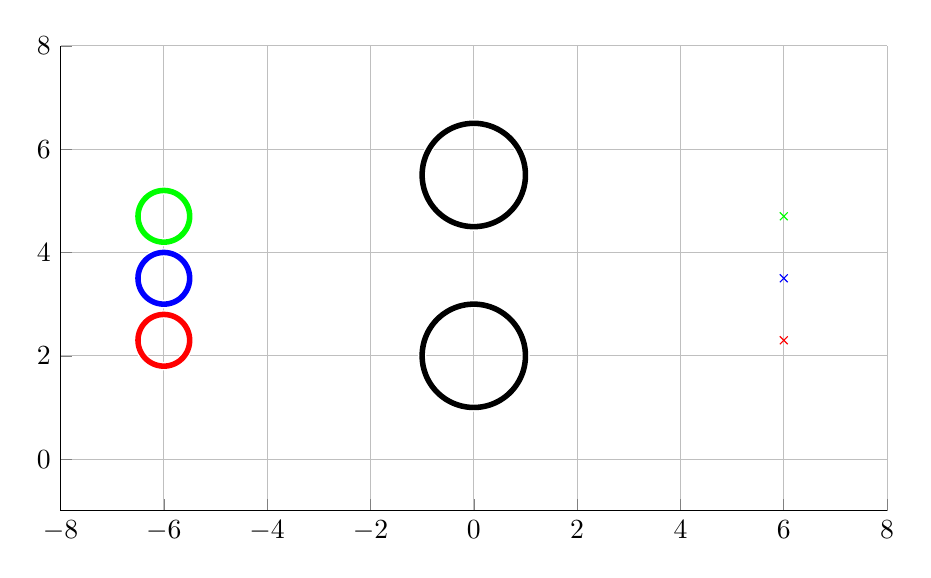
\begin{tikzpicture}

\begin{axis}[%
width=4.133in,
height=2.325in,
at={(0.693in,0.907in)},
scale only axis,
unbounded coords=jump,
xmin=-8,
xmax=8,
xmajorgrids,
ymin=-1,
ymax=8,
ymajorgrids,
axis background/.style={fill=white},
axis x line*=bottom,
axis y line*=left
]
\addplot [color=blue,only marks,mark=x,mark options={solid},forget plot]
  table[row sep=crcr]{%
6	3.5\\
};
\addplot [color=red,only marks,mark=x,mark options={solid},forget plot]
  table[row sep=crcr]{%
6	2.3\\
};
\addplot [color=green,only marks,mark=x,mark options={solid},forget plot]
  table[row sep=crcr]{%
6	4.7\\
};
\addplot [color=white,solid,line width=3.0pt,forget plot]
  table[row sep=crcr]{%
-5.5	3.5\\
-5.50030458649045	3.51744974835125\\
-5.50121797487009	3.53487823687206\\
-5.50273905231586	3.55226423163383\\
-5.50486596562921	3.56958655048003\\
-5.5075961234939	3.58682408883347\\
-5.5109261996331	3.60395584540888\\
-5.514852136862	3.62096094779983\\
-5.51936915203084	3.6378186779085\\
-5.52447174185242	3.65450849718747\\
-5.53015368960705	3.67101007166283\\
-5.53640807271661	3.68730329670796\\
-5.5432272711787	3.7033683215379\\
-5.55060297685042	3.71918557339454\\
-5.55852620357054	3.73473578139295\\
-5.56698729810778	3.75\\
-5.57597595192179	3.7649596321166\\
-5.58548121372248	3.77959645173537\\
-5.59549150281253	3.79389262614624\\
-5.60599462319664	3.80783073766283\\
-5.61697777844051	3.82139380484327\\
-5.6284275872613	3.83456530317943\\
-5.64033009983067	3.8473291852295\\
-5.6526708147705	3.85966990016933\\
-5.66543469682057	3.8715724127387\\
-5.67860619515673	3.88302222155949\\
-5.69216926233717	3.89400537680336\\
-5.70610737385376	3.90450849718747\\
-5.72040354826463	3.91451878627752\\
-5.7350403678834	3.92402404807821\\
-5.75	3.93301270189222\\
-5.76526421860705	3.94147379642946\\
-5.78081442660546	3.94939702314958\\
-5.7966316784621	3.9567727288213\\
-5.81269670329204	3.96359192728339\\
-5.82898992833717	3.96984631039295\\
-5.84549150281253	3.97552825814758\\
-5.8621813220915	3.98063084796916\\
-5.87903905220017	3.985147863138\\
-5.89604415459112	3.9890738003669\\
-5.91317591116653	3.9924038765061\\
-5.93041344951997	3.99513403437079\\
-5.94773576836617	3.99726094768414\\
-5.96512176312794	3.99878202512991\\
-5.98255025164875	3.99969541350955\\
-6	4\\
-6.01744974835125	3.99969541350955\\
-6.03487823687206	3.99878202512991\\
-6.05226423163383	3.99726094768414\\
-6.06958655048003	3.99513403437079\\
-6.08682408883347	3.9924038765061\\
-6.10395584540888	3.9890738003669\\
-6.12096094779983	3.985147863138\\
-6.1378186779085	3.98063084796916\\
-6.15450849718747	3.97552825814758\\
-6.17101007166283	3.96984631039295\\
-6.18730329670796	3.96359192728339\\
-6.2033683215379	3.9567727288213\\
-6.21918557339454	3.94939702314958\\
-6.23473578139295	3.94147379642946\\
-6.25	3.93301270189222\\
-6.2649596321166	3.92402404807821\\
-6.27959645173537	3.91451878627752\\
-6.29389262614624	3.90450849718747\\
-6.30783073766283	3.89400537680336\\
-6.32139380484327	3.88302222155949\\
-6.33456530317943	3.8715724127387\\
-6.3473291852295	3.85966990016933\\
-6.35966990016933	3.8473291852295\\
-6.3715724127387	3.83456530317943\\
-6.38302222155949	3.82139380484327\\
-6.39400537680336	3.80783073766283\\
-6.40450849718747	3.79389262614624\\
-6.41451878627752	3.77959645173537\\
-6.42402404807821	3.7649596321166\\
-6.43301270189222	3.75\\
-6.44147379642946	3.73473578139295\\
-6.44939702314958	3.71918557339454\\
-6.4567727288213	3.7033683215379\\
-6.46359192728339	3.68730329670796\\
-6.46984631039295	3.67101007166283\\
-6.47552825814758	3.65450849718747\\
-6.48063084796916	3.6378186779085\\
-6.485147863138	3.62096094779983\\
-6.4890738003669	3.60395584540888\\
-6.4924038765061	3.58682408883347\\
-6.49513403437079	3.56958655048003\\
-6.49726094768414	3.55226423163383\\
-6.49878202512991	3.53487823687206\\
-6.49969541350955	3.51744974835125\\
-6.5	3.5\\
-6.49969541350955	3.48255025164875\\
-6.49878202512991	3.46512176312794\\
-6.49726094768414	3.44773576836617\\
-6.49513403437079	3.43041344951997\\
-6.4924038765061	3.41317591116653\\
-6.4890738003669	3.39604415459112\\
-6.485147863138	3.37903905220017\\
-6.48063084796916	3.3621813220915\\
-6.47552825814758	3.34549150281253\\
-6.46984631039295	3.32898992833717\\
-6.46359192728339	3.31269670329204\\
-6.4567727288213	3.2966316784621\\
-6.44939702314958	3.28081442660546\\
-6.44147379642946	3.26526421860705\\
-6.43301270189222	3.25\\
-6.42402404807821	3.2350403678834\\
-6.41451878627752	3.22040354826463\\
-6.40450849718747	3.20610737385376\\
-6.39400537680336	3.19216926233717\\
-6.38302222155949	3.17860619515673\\
-6.3715724127387	3.16543469682057\\
-6.35966990016933	3.1526708147705\\
-6.3473291852295	3.14033009983067\\
-6.33456530317943	3.1284275872613\\
-6.32139380484327	3.11697777844051\\
-6.30783073766283	3.10599462319664\\
-6.29389262614624	3.09549150281253\\
-6.27959645173537	3.08548121372248\\
-6.2649596321166	3.07597595192179\\
-6.25	3.06698729810778\\
-6.23473578139295	3.05852620357054\\
-6.21918557339454	3.05060297685042\\
-6.2033683215379	3.0432272711787\\
-6.18730329670796	3.03640807271661\\
-6.17101007166283	3.03015368960705\\
-6.15450849718747	3.02447174185242\\
-6.1378186779085	3.01936915203084\\
-6.12096094779983	3.014852136862\\
-6.10395584540888	3.0109261996331\\
-6.08682408883347	3.0075961234939\\
-6.06958655048003	3.00486596562921\\
-6.05226423163383	3.00273905231586\\
-6.03487823687206	3.00121797487009\\
-6.01744974835125	3.00030458649045\\
-6	3\\
-5.98255025164875	3.00030458649045\\
-5.96512176312794	3.00121797487009\\
-5.94773576836617	3.00273905231586\\
-5.93041344951997	3.00486596562921\\
-5.91317591116653	3.0075961234939\\
-5.89604415459112	3.0109261996331\\
-5.87903905220017	3.014852136862\\
-5.8621813220915	3.01936915203084\\
-5.84549150281253	3.02447174185242\\
-5.82898992833717	3.03015368960705\\
-5.81269670329204	3.03640807271661\\
-5.7966316784621	3.0432272711787\\
-5.78081442660546	3.05060297685042\\
-5.76526421860705	3.05852620357054\\
-5.75	3.06698729810778\\
-5.7350403678834	3.07597595192179\\
-5.72040354826463	3.08548121372248\\
-5.70610737385376	3.09549150281253\\
-5.69216926233717	3.10599462319664\\
-5.67860619515673	3.11697777844051\\
-5.66543469682057	3.1284275872613\\
-5.6526708147705	3.14033009983067\\
-5.64033009983067	3.1526708147705\\
-5.6284275872613	3.16543469682057\\
-5.61697777844051	3.17860619515673\\
-5.60599462319664	3.19216926233717\\
-5.59549150281253	3.20610737385376\\
-5.58548121372248	3.22040354826463\\
-5.57597595192179	3.2350403678834\\
-5.56698729810778	3.25\\
-5.55852620357054	3.26526421860705\\
-5.55060297685042	3.28081442660546\\
-5.5432272711787	3.2966316784621\\
-5.53640807271661	3.31269670329204\\
-5.53015368960705	3.32898992833717\\
-5.52447174185242	3.34549150281253\\
-5.51936915203084	3.3621813220915\\
-5.514852136862	3.37903905220017\\
-5.5109261996331	3.39604415459112\\
-5.5075961234939	3.41317591116653\\
-5.50486596562921	3.43041344951997\\
-5.50273905231586	3.44773576836617\\
-5.50121797487009	3.46512176312794\\
-5.50030458649045	3.48255025164875\\
-5.5	3.5\\
nan	nan\\
};
\addplot [color=blue,solid,line width=2.0pt,forget plot]
  table[row sep=crcr]{%
-5.5	3.5\\
-5.50030458649045	3.51744974835125\\
-5.50121797487009	3.53487823687206\\
-5.50273905231586	3.55226423163383\\
-5.50486596562921	3.56958655048003\\
-5.5075961234939	3.58682408883347\\
-5.5109261996331	3.60395584540888\\
-5.514852136862	3.62096094779983\\
-5.51936915203084	3.6378186779085\\
-5.52447174185242	3.65450849718747\\
-5.53015368960705	3.67101007166283\\
-5.53640807271661	3.68730329670796\\
-5.5432272711787	3.7033683215379\\
-5.55060297685042	3.71918557339454\\
-5.55852620357054	3.73473578139295\\
-5.56698729810778	3.75\\
-5.57597595192179	3.7649596321166\\
-5.58548121372248	3.77959645173537\\
-5.59549150281253	3.79389262614624\\
-5.60599462319664	3.80783073766283\\
-5.61697777844051	3.82139380484327\\
-5.6284275872613	3.83456530317943\\
-5.64033009983067	3.8473291852295\\
-5.6526708147705	3.85966990016933\\
-5.66543469682057	3.8715724127387\\
-5.67860619515673	3.88302222155949\\
-5.69216926233717	3.89400537680336\\
-5.70610737385376	3.90450849718747\\
-5.72040354826463	3.91451878627752\\
-5.7350403678834	3.92402404807821\\
-5.75	3.93301270189222\\
-5.76526421860705	3.94147379642946\\
-5.78081442660546	3.94939702314958\\
-5.7966316784621	3.9567727288213\\
-5.81269670329204	3.96359192728339\\
-5.82898992833717	3.96984631039295\\
-5.84549150281253	3.97552825814758\\
-5.8621813220915	3.98063084796916\\
-5.87903905220017	3.985147863138\\
-5.89604415459112	3.9890738003669\\
-5.91317591116653	3.9924038765061\\
-5.93041344951997	3.99513403437079\\
-5.94773576836617	3.99726094768414\\
-5.96512176312794	3.99878202512991\\
-5.98255025164875	3.99969541350955\\
-6	4\\
-6.01744974835125	3.99969541350955\\
-6.03487823687206	3.99878202512991\\
-6.05226423163383	3.99726094768414\\
-6.06958655048003	3.99513403437079\\
-6.08682408883347	3.9924038765061\\
-6.10395584540888	3.9890738003669\\
-6.12096094779983	3.985147863138\\
-6.1378186779085	3.98063084796916\\
-6.15450849718747	3.97552825814758\\
-6.17101007166283	3.96984631039295\\
-6.18730329670796	3.96359192728339\\
-6.2033683215379	3.9567727288213\\
-6.21918557339454	3.94939702314958\\
-6.23473578139295	3.94147379642946\\
-6.25	3.93301270189222\\
-6.2649596321166	3.92402404807821\\
-6.27959645173537	3.91451878627752\\
-6.29389262614624	3.90450849718747\\
-6.30783073766283	3.89400537680336\\
-6.32139380484327	3.88302222155949\\
-6.33456530317943	3.8715724127387\\
-6.3473291852295	3.85966990016933\\
-6.35966990016933	3.8473291852295\\
-6.3715724127387	3.83456530317943\\
-6.38302222155949	3.82139380484327\\
-6.39400537680336	3.80783073766283\\
-6.40450849718747	3.79389262614624\\
-6.41451878627752	3.77959645173537\\
-6.42402404807821	3.7649596321166\\
-6.43301270189222	3.75\\
-6.44147379642946	3.73473578139295\\
-6.44939702314958	3.71918557339454\\
-6.4567727288213	3.7033683215379\\
-6.46359192728339	3.68730329670796\\
-6.46984631039295	3.67101007166283\\
-6.47552825814758	3.65450849718747\\
-6.48063084796916	3.6378186779085\\
-6.485147863138	3.62096094779983\\
-6.4890738003669	3.60395584540888\\
-6.4924038765061	3.58682408883347\\
-6.49513403437079	3.56958655048003\\
-6.49726094768414	3.55226423163383\\
-6.49878202512991	3.53487823687206\\
-6.49969541350955	3.51744974835125\\
-6.5	3.5\\
-6.49969541350955	3.48255025164875\\
-6.49878202512991	3.46512176312794\\
-6.49726094768414	3.44773576836617\\
-6.49513403437079	3.43041344951997\\
-6.4924038765061	3.41317591116653\\
-6.4890738003669	3.39604415459112\\
-6.485147863138	3.37903905220017\\
-6.48063084796916	3.3621813220915\\
-6.47552825814758	3.34549150281253\\
-6.46984631039295	3.32898992833717\\
-6.46359192728339	3.31269670329204\\
-6.4567727288213	3.2966316784621\\
-6.44939702314958	3.28081442660546\\
-6.44147379642946	3.26526421860705\\
-6.43301270189222	3.25\\
-6.42402404807821	3.2350403678834\\
-6.41451878627752	3.22040354826463\\
-6.40450849718747	3.20610737385376\\
-6.39400537680336	3.19216926233717\\
-6.38302222155949	3.17860619515673\\
-6.3715724127387	3.16543469682057\\
-6.35966990016933	3.1526708147705\\
-6.3473291852295	3.14033009983067\\
-6.33456530317943	3.1284275872613\\
-6.32139380484327	3.11697777844051\\
-6.30783073766283	3.10599462319664\\
-6.29389262614624	3.09549150281253\\
-6.27959645173537	3.08548121372248\\
-6.2649596321166	3.07597595192179\\
-6.25	3.06698729810778\\
-6.23473578139295	3.05852620357054\\
-6.21918557339454	3.05060297685042\\
-6.2033683215379	3.0432272711787\\
-6.18730329670796	3.03640807271661\\
-6.17101007166283	3.03015368960705\\
-6.15450849718747	3.02447174185242\\
-6.1378186779085	3.01936915203084\\
-6.12096094779983	3.014852136862\\
-6.10395584540888	3.0109261996331\\
-6.08682408883347	3.0075961234939\\
-6.06958655048003	3.00486596562921\\
-6.05226423163383	3.00273905231586\\
-6.03487823687206	3.00121797487009\\
-6.01744974835125	3.00030458649045\\
-6	3\\
-5.98255025164875	3.00030458649045\\
-5.96512176312794	3.00121797487009\\
-5.94773576836617	3.00273905231586\\
-5.93041344951997	3.00486596562921\\
-5.91317591116653	3.0075961234939\\
-5.89604415459112	3.0109261996331\\
-5.87903905220017	3.014852136862\\
-5.8621813220915	3.01936915203084\\
-5.84549150281253	3.02447174185242\\
-5.82898992833717	3.03015368960705\\
-5.81269670329204	3.03640807271661\\
-5.7966316784621	3.0432272711787\\
-5.78081442660546	3.05060297685042\\
-5.76526421860705	3.05852620357054\\
-5.75	3.06698729810778\\
-5.7350403678834	3.07597595192179\\
-5.72040354826463	3.08548121372248\\
-5.70610737385376	3.09549150281253\\
-5.69216926233717	3.10599462319664\\
-5.67860619515673	3.11697777844051\\
-5.66543469682057	3.1284275872613\\
-5.6526708147705	3.14033009983067\\
-5.64033009983067	3.1526708147705\\
-5.6284275872613	3.16543469682057\\
-5.61697777844051	3.17860619515673\\
-5.60599462319664	3.19216926233717\\
-5.59549150281253	3.20610737385376\\
-5.58548121372248	3.22040354826463\\
-5.57597595192179	3.2350403678834\\
-5.56698729810778	3.25\\
-5.55852620357054	3.26526421860705\\
-5.55060297685042	3.28081442660546\\
-5.5432272711787	3.2966316784621\\
-5.53640807271661	3.31269670329204\\
-5.53015368960705	3.32898992833717\\
-5.52447174185242	3.34549150281253\\
-5.51936915203084	3.3621813220915\\
-5.514852136862	3.37903905220017\\
-5.5109261996331	3.39604415459112\\
-5.5075961234939	3.41317591116653\\
-5.50486596562921	3.43041344951997\\
-5.50273905231586	3.44773576836617\\
-5.50121797487009	3.46512176312794\\
-5.50030458649045	3.48255025164875\\
-5.5	3.5\\
nan	nan\\
};
\addplot [color=white,solid,line width=3.0pt,forget plot]
  table[row sep=crcr]{%
-5.5	2.3\\
-5.50030458649045	2.31744974835125\\
-5.50121797487009	2.33487823687206\\
-5.50273905231586	2.35226423163383\\
-5.50486596562921	2.36958655048003\\
-5.5075961234939	2.38682408883346\\
-5.5109261996331	2.40395584540888\\
-5.514852136862	2.42096094779983\\
-5.51936915203084	2.4378186779085\\
-5.52447174185242	2.45450849718747\\
-5.53015368960705	2.47101007166283\\
-5.53640807271661	2.48730329670796\\
-5.5432272711787	2.5033683215379\\
-5.55060297685042	2.51918557339454\\
-5.55852620357054	2.53473578139295\\
-5.56698729810778	2.55\\
-5.57597595192179	2.5649596321166\\
-5.58548121372248	2.57959645173537\\
-5.59549150281253	2.59389262614624\\
-5.60599462319664	2.60783073766283\\
-5.61697777844051	2.62139380484327\\
-5.6284275872613	2.63456530317943\\
-5.64033009983067	2.6473291852295\\
-5.6526708147705	2.65966990016933\\
-5.66543469682057	2.6715724127387\\
-5.67860619515673	2.68302222155949\\
-5.69216926233717	2.69400537680336\\
-5.70610737385376	2.70450849718747\\
-5.72040354826463	2.71451878627752\\
-5.7350403678834	2.72402404807821\\
-5.75	2.73301270189222\\
-5.76526421860705	2.74147379642946\\
-5.78081442660546	2.74939702314958\\
-5.7966316784621	2.7567727288213\\
-5.81269670329204	2.76359192728339\\
-5.82898992833717	2.76984631039295\\
-5.84549150281253	2.77552825814758\\
-5.8621813220915	2.78063084796916\\
-5.87903905220017	2.785147863138\\
-5.89604415459112	2.7890738003669\\
-5.91317591116653	2.7924038765061\\
-5.93041344951997	2.79513403437078\\
-5.94773576836617	2.79726094768414\\
-5.96512176312794	2.79878202512991\\
-5.98255025164875	2.79969541350955\\
-6	2.8\\
-6.01744974835125	2.79969541350955\\
-6.03487823687206	2.79878202512991\\
-6.05226423163383	2.79726094768414\\
-6.06958655048003	2.79513403437078\\
-6.08682408883347	2.7924038765061\\
-6.10395584540888	2.7890738003669\\
-6.12096094779983	2.785147863138\\
-6.1378186779085	2.78063084796916\\
-6.15450849718747	2.77552825814758\\
-6.17101007166283	2.76984631039295\\
-6.18730329670796	2.76359192728339\\
-6.2033683215379	2.7567727288213\\
-6.21918557339454	2.74939702314958\\
-6.23473578139295	2.74147379642946\\
-6.25	2.73301270189222\\
-6.2649596321166	2.72402404807821\\
-6.27959645173537	2.71451878627752\\
-6.29389262614624	2.70450849718747\\
-6.30783073766283	2.69400537680336\\
-6.32139380484327	2.68302222155949\\
-6.33456530317943	2.6715724127387\\
-6.3473291852295	2.65966990016933\\
-6.35966990016933	2.6473291852295\\
-6.3715724127387	2.63456530317943\\
-6.38302222155949	2.62139380484327\\
-6.39400537680336	2.60783073766283\\
-6.40450849718747	2.59389262614624\\
-6.41451878627752	2.57959645173537\\
-6.42402404807821	2.5649596321166\\
-6.43301270189222	2.55\\
-6.44147379642946	2.53473578139295\\
-6.44939702314958	2.51918557339454\\
-6.4567727288213	2.5033683215379\\
-6.46359192728339	2.48730329670796\\
-6.46984631039295	2.47101007166283\\
-6.47552825814758	2.45450849718747\\
-6.48063084796916	2.4378186779085\\
-6.485147863138	2.42096094779983\\
-6.4890738003669	2.40395584540888\\
-6.4924038765061	2.38682408883346\\
-6.49513403437079	2.36958655048003\\
-6.49726094768414	2.35226423163383\\
-6.49878202512991	2.33487823687206\\
-6.49969541350955	2.31744974835125\\
-6.5	2.3\\
-6.49969541350955	2.28255025164875\\
-6.49878202512991	2.26512176312794\\
-6.49726094768414	2.24773576836617\\
-6.49513403437079	2.23041344951997\\
-6.4924038765061	2.21317591116653\\
-6.4890738003669	2.19604415459112\\
-6.485147863138	2.17903905220017\\
-6.48063084796916	2.1621813220915\\
-6.47552825814758	2.14549150281253\\
-6.46984631039295	2.12898992833717\\
-6.46359192728339	2.11269670329204\\
-6.4567727288213	2.0966316784621\\
-6.44939702314958	2.08081442660546\\
-6.44147379642946	2.06526421860705\\
-6.43301270189222	2.05\\
-6.42402404807821	2.0350403678834\\
-6.41451878627752	2.02040354826463\\
-6.40450849718747	2.00610737385376\\
-6.39400537680336	1.99216926233717\\
-6.38302222155949	1.97860619515673\\
-6.3715724127387	1.96543469682057\\
-6.35966990016933	1.9526708147705\\
-6.3473291852295	1.94033009983067\\
-6.33456530317943	1.9284275872613\\
-6.32139380484327	1.91697777844051\\
-6.30783073766283	1.90599462319664\\
-6.29389262614624	1.89549150281253\\
-6.27959645173537	1.88548121372248\\
-6.2649596321166	1.87597595192179\\
-6.25	1.86698729810778\\
-6.23473578139295	1.85852620357054\\
-6.21918557339454	1.85060297685042\\
-6.2033683215379	1.8432272711787\\
-6.18730329670796	1.83640807271661\\
-6.17101007166283	1.83015368960705\\
-6.15450849718747	1.82447174185242\\
-6.1378186779085	1.81936915203084\\
-6.12096094779983	1.814852136862\\
-6.10395584540888	1.8109261996331\\
-6.08682408883347	1.8075961234939\\
-6.06958655048003	1.80486596562921\\
-6.05226423163383	1.80273905231586\\
-6.03487823687206	1.80121797487009\\
-6.01744974835125	1.80030458649045\\
-6	1.8\\
-5.98255025164875	1.80030458649045\\
-5.96512176312794	1.80121797487009\\
-5.94773576836617	1.80273905231586\\
-5.93041344951997	1.80486596562921\\
-5.91317591116653	1.8075961234939\\
-5.89604415459112	1.8109261996331\\
-5.87903905220017	1.814852136862\\
-5.8621813220915	1.81936915203084\\
-5.84549150281253	1.82447174185242\\
-5.82898992833717	1.83015368960705\\
-5.81269670329204	1.83640807271661\\
-5.7966316784621	1.8432272711787\\
-5.78081442660546	1.85060297685042\\
-5.76526421860705	1.85852620357054\\
-5.75	1.86698729810778\\
-5.7350403678834	1.87597595192179\\
-5.72040354826463	1.88548121372248\\
-5.70610737385376	1.89549150281253\\
-5.69216926233717	1.90599462319664\\
-5.67860619515673	1.91697777844051\\
-5.66543469682057	1.9284275872613\\
-5.6526708147705	1.94033009983067\\
-5.64033009983067	1.9526708147705\\
-5.6284275872613	1.96543469682057\\
-5.61697777844051	1.97860619515673\\
-5.60599462319664	1.99216926233717\\
-5.59549150281253	2.00610737385376\\
-5.58548121372248	2.02040354826463\\
-5.57597595192179	2.0350403678834\\
-5.56698729810778	2.05\\
-5.55852620357054	2.06526421860705\\
-5.55060297685042	2.08081442660546\\
-5.5432272711787	2.0966316784621\\
-5.53640807271661	2.11269670329204\\
-5.53015368960705	2.12898992833717\\
-5.52447174185242	2.14549150281253\\
-5.51936915203084	2.1621813220915\\
-5.514852136862	2.17903905220017\\
-5.5109261996331	2.19604415459112\\
-5.5075961234939	2.21317591116653\\
-5.50486596562921	2.23041344951997\\
-5.50273905231586	2.24773576836617\\
-5.50121797487009	2.26512176312794\\
-5.50030458649045	2.28255025164875\\
-5.5	2.3\\
nan	nan\\
};
\addplot [color=red,solid,line width=2.0pt,forget plot]
  table[row sep=crcr]{%
-5.5	2.3\\
-5.50030458649045	2.31744974835125\\
-5.50121797487009	2.33487823687206\\
-5.50273905231586	2.35226423163383\\
-5.50486596562921	2.36958655048003\\
-5.5075961234939	2.38682408883346\\
-5.5109261996331	2.40395584540888\\
-5.514852136862	2.42096094779983\\
-5.51936915203084	2.4378186779085\\
-5.52447174185242	2.45450849718747\\
-5.53015368960705	2.47101007166283\\
-5.53640807271661	2.48730329670796\\
-5.5432272711787	2.5033683215379\\
-5.55060297685042	2.51918557339454\\
-5.55852620357054	2.53473578139295\\
-5.56698729810778	2.55\\
-5.57597595192179	2.5649596321166\\
-5.58548121372248	2.57959645173537\\
-5.59549150281253	2.59389262614624\\
-5.60599462319664	2.60783073766283\\
-5.61697777844051	2.62139380484327\\
-5.6284275872613	2.63456530317943\\
-5.64033009983067	2.6473291852295\\
-5.6526708147705	2.65966990016933\\
-5.66543469682057	2.6715724127387\\
-5.67860619515673	2.68302222155949\\
-5.69216926233717	2.69400537680336\\
-5.70610737385376	2.70450849718747\\
-5.72040354826463	2.71451878627752\\
-5.7350403678834	2.72402404807821\\
-5.75	2.73301270189222\\
-5.76526421860705	2.74147379642946\\
-5.78081442660546	2.74939702314958\\
-5.7966316784621	2.7567727288213\\
-5.81269670329204	2.76359192728339\\
-5.82898992833717	2.76984631039295\\
-5.84549150281253	2.77552825814758\\
-5.8621813220915	2.78063084796916\\
-5.87903905220017	2.785147863138\\
-5.89604415459112	2.7890738003669\\
-5.91317591116653	2.7924038765061\\
-5.93041344951997	2.79513403437078\\
-5.94773576836617	2.79726094768414\\
-5.96512176312794	2.79878202512991\\
-5.98255025164875	2.79969541350955\\
-6	2.8\\
-6.01744974835125	2.79969541350955\\
-6.03487823687206	2.79878202512991\\
-6.05226423163383	2.79726094768414\\
-6.06958655048003	2.79513403437078\\
-6.08682408883347	2.7924038765061\\
-6.10395584540888	2.7890738003669\\
-6.12096094779983	2.785147863138\\
-6.1378186779085	2.78063084796916\\
-6.15450849718747	2.77552825814758\\
-6.17101007166283	2.76984631039295\\
-6.18730329670796	2.76359192728339\\
-6.2033683215379	2.7567727288213\\
-6.21918557339454	2.74939702314958\\
-6.23473578139295	2.74147379642946\\
-6.25	2.73301270189222\\
-6.2649596321166	2.72402404807821\\
-6.27959645173537	2.71451878627752\\
-6.29389262614624	2.70450849718747\\
-6.30783073766283	2.69400537680336\\
-6.32139380484327	2.68302222155949\\
-6.33456530317943	2.6715724127387\\
-6.3473291852295	2.65966990016933\\
-6.35966990016933	2.6473291852295\\
-6.3715724127387	2.63456530317943\\
-6.38302222155949	2.62139380484327\\
-6.39400537680336	2.60783073766283\\
-6.40450849718747	2.59389262614624\\
-6.41451878627752	2.57959645173537\\
-6.42402404807821	2.5649596321166\\
-6.43301270189222	2.55\\
-6.44147379642946	2.53473578139295\\
-6.44939702314958	2.51918557339454\\
-6.4567727288213	2.5033683215379\\
-6.46359192728339	2.48730329670796\\
-6.46984631039295	2.47101007166283\\
-6.47552825814758	2.45450849718747\\
-6.48063084796916	2.4378186779085\\
-6.485147863138	2.42096094779983\\
-6.4890738003669	2.40395584540888\\
-6.4924038765061	2.38682408883346\\
-6.49513403437079	2.36958655048003\\
-6.49726094768414	2.35226423163383\\
-6.49878202512991	2.33487823687206\\
-6.49969541350955	2.31744974835125\\
-6.5	2.3\\
-6.49969541350955	2.28255025164875\\
-6.49878202512991	2.26512176312794\\
-6.49726094768414	2.24773576836617\\
-6.49513403437079	2.23041344951997\\
-6.4924038765061	2.21317591116653\\
-6.4890738003669	2.19604415459112\\
-6.485147863138	2.17903905220017\\
-6.48063084796916	2.1621813220915\\
-6.47552825814758	2.14549150281253\\
-6.46984631039295	2.12898992833717\\
-6.46359192728339	2.11269670329204\\
-6.4567727288213	2.0966316784621\\
-6.44939702314958	2.08081442660546\\
-6.44147379642946	2.06526421860705\\
-6.43301270189222	2.05\\
-6.42402404807821	2.0350403678834\\
-6.41451878627752	2.02040354826463\\
-6.40450849718747	2.00610737385376\\
-6.39400537680336	1.99216926233717\\
-6.38302222155949	1.97860619515673\\
-6.3715724127387	1.96543469682057\\
-6.35966990016933	1.9526708147705\\
-6.3473291852295	1.94033009983067\\
-6.33456530317943	1.9284275872613\\
-6.32139380484327	1.91697777844051\\
-6.30783073766283	1.90599462319664\\
-6.29389262614624	1.89549150281253\\
-6.27959645173537	1.88548121372248\\
-6.2649596321166	1.87597595192179\\
-6.25	1.86698729810778\\
-6.23473578139295	1.85852620357054\\
-6.21918557339454	1.85060297685042\\
-6.2033683215379	1.8432272711787\\
-6.18730329670796	1.83640807271661\\
-6.17101007166283	1.83015368960705\\
-6.15450849718747	1.82447174185242\\
-6.1378186779085	1.81936915203084\\
-6.12096094779983	1.814852136862\\
-6.10395584540888	1.8109261996331\\
-6.08682408883347	1.8075961234939\\
-6.06958655048003	1.80486596562921\\
-6.05226423163383	1.80273905231586\\
-6.03487823687206	1.80121797487009\\
-6.01744974835125	1.80030458649045\\
-6	1.8\\
-5.98255025164875	1.80030458649045\\
-5.96512176312794	1.80121797487009\\
-5.94773576836617	1.80273905231586\\
-5.93041344951997	1.80486596562921\\
-5.91317591116653	1.8075961234939\\
-5.89604415459112	1.8109261996331\\
-5.87903905220017	1.814852136862\\
-5.8621813220915	1.81936915203084\\
-5.84549150281253	1.82447174185242\\
-5.82898992833717	1.83015368960705\\
-5.81269670329204	1.83640807271661\\
-5.7966316784621	1.8432272711787\\
-5.78081442660546	1.85060297685042\\
-5.76526421860705	1.85852620357054\\
-5.75	1.86698729810778\\
-5.7350403678834	1.87597595192179\\
-5.72040354826463	1.88548121372248\\
-5.70610737385376	1.89549150281253\\
-5.69216926233717	1.90599462319664\\
-5.67860619515673	1.91697777844051\\
-5.66543469682057	1.9284275872613\\
-5.6526708147705	1.94033009983067\\
-5.64033009983067	1.9526708147705\\
-5.6284275872613	1.96543469682057\\
-5.61697777844051	1.97860619515673\\
-5.60599462319664	1.99216926233717\\
-5.59549150281253	2.00610737385376\\
-5.58548121372248	2.02040354826463\\
-5.57597595192179	2.0350403678834\\
-5.56698729810778	2.05\\
-5.55852620357054	2.06526421860705\\
-5.55060297685042	2.08081442660546\\
-5.5432272711787	2.0966316784621\\
-5.53640807271661	2.11269670329204\\
-5.53015368960705	2.12898992833717\\
-5.52447174185242	2.14549150281253\\
-5.51936915203084	2.1621813220915\\
-5.514852136862	2.17903905220017\\
-5.5109261996331	2.19604415459112\\
-5.5075961234939	2.21317591116653\\
-5.50486596562921	2.23041344951997\\
-5.50273905231586	2.24773576836617\\
-5.50121797487009	2.26512176312794\\
-5.50030458649045	2.28255025164875\\
-5.5	2.3\\
nan	nan\\
};
\addplot [color=white,solid,line width=3.0pt,forget plot]
  table[row sep=crcr]{%
-5.5	4.7\\
-5.50030458649045	4.71744974835125\\
-5.50121797487009	4.73487823687206\\
-5.50273905231586	4.75226423163383\\
-5.50486596562921	4.76958655048003\\
-5.5075961234939	4.78682408883347\\
-5.5109261996331	4.80395584540888\\
-5.514852136862	4.82096094779983\\
-5.51936915203084	4.8378186779085\\
-5.52447174185242	4.85450849718747\\
-5.53015368960705	4.87101007166283\\
-5.53640807271661	4.88730329670796\\
-5.5432272711787	4.9033683215379\\
-5.55060297685042	4.91918557339454\\
-5.55852620357054	4.93473578139295\\
-5.56698729810778	4.95\\
-5.57597595192179	4.9649596321166\\
-5.58548121372248	4.97959645173537\\
-5.59549150281253	4.99389262614624\\
-5.60599462319664	5.00783073766283\\
-5.61697777844051	5.02139380484327\\
-5.6284275872613	5.03456530317943\\
-5.64033009983067	5.0473291852295\\
-5.6526708147705	5.05966990016933\\
-5.66543469682057	5.0715724127387\\
-5.67860619515673	5.08302222155949\\
-5.69216926233717	5.09400537680336\\
-5.70610737385376	5.10450849718747\\
-5.72040354826463	5.11451878627752\\
-5.7350403678834	5.12402404807821\\
-5.75	5.13301270189222\\
-5.76526421860705	5.14147379642946\\
-5.78081442660546	5.14939702314958\\
-5.7966316784621	5.1567727288213\\
-5.81269670329204	5.16359192728339\\
-5.82898992833717	5.16984631039295\\
-5.84549150281253	5.17552825814758\\
-5.8621813220915	5.18063084796916\\
-5.87903905220017	5.185147863138\\
-5.89604415459112	5.1890738003669\\
-5.91317591116653	5.1924038765061\\
-5.93041344951997	5.19513403437079\\
-5.94773576836617	5.19726094768414\\
-5.96512176312794	5.19878202512991\\
-5.98255025164875	5.19969541350955\\
-6	5.2\\
-6.01744974835125	5.19969541350955\\
-6.03487823687206	5.19878202512991\\
-6.05226423163383	5.19726094768414\\
-6.06958655048003	5.19513403437079\\
-6.08682408883347	5.1924038765061\\
-6.10395584540888	5.1890738003669\\
-6.12096094779983	5.185147863138\\
-6.1378186779085	5.18063084796916\\
-6.15450849718747	5.17552825814758\\
-6.17101007166283	5.16984631039295\\
-6.18730329670796	5.16359192728339\\
-6.2033683215379	5.1567727288213\\
-6.21918557339454	5.14939702314958\\
-6.23473578139295	5.14147379642946\\
-6.25	5.13301270189222\\
-6.2649596321166	5.12402404807821\\
-6.27959645173537	5.11451878627752\\
-6.29389262614624	5.10450849718747\\
-6.30783073766283	5.09400537680336\\
-6.32139380484327	5.08302222155949\\
-6.33456530317943	5.0715724127387\\
-6.3473291852295	5.05966990016933\\
-6.35966990016933	5.0473291852295\\
-6.3715724127387	5.03456530317943\\
-6.38302222155949	5.02139380484327\\
-6.39400537680336	5.00783073766283\\
-6.40450849718747	4.99389262614624\\
-6.41451878627752	4.97959645173537\\
-6.42402404807821	4.9649596321166\\
-6.43301270189222	4.95\\
-6.44147379642946	4.93473578139295\\
-6.44939702314958	4.91918557339454\\
-6.4567727288213	4.9033683215379\\
-6.46359192728339	4.88730329670796\\
-6.46984631039295	4.87101007166283\\
-6.47552825814758	4.85450849718747\\
-6.48063084796916	4.8378186779085\\
-6.485147863138	4.82096094779983\\
-6.4890738003669	4.80395584540888\\
-6.4924038765061	4.78682408883347\\
-6.49513403437079	4.76958655048003\\
-6.49726094768414	4.75226423163383\\
-6.49878202512991	4.73487823687206\\
-6.49969541350955	4.71744974835125\\
-6.5	4.7\\
-6.49969541350955	4.68255025164875\\
-6.49878202512991	4.66512176312794\\
-6.49726094768414	4.64773576836617\\
-6.49513403437079	4.63041344951997\\
-6.4924038765061	4.61317591116654\\
-6.4890738003669	4.59604415459112\\
-6.485147863138	4.57903905220017\\
-6.48063084796916	4.5621813220915\\
-6.47552825814758	4.54549150281253\\
-6.46984631039295	4.52898992833717\\
-6.46359192728339	4.51269670329204\\
-6.4567727288213	4.4966316784621\\
-6.44939702314958	4.48081442660546\\
-6.44147379642946	4.46526421860705\\
-6.43301270189222	4.45\\
-6.42402404807821	4.4350403678834\\
-6.41451878627752	4.42040354826463\\
-6.40450849718747	4.40610737385376\\
-6.39400537680336	4.39216926233717\\
-6.38302222155949	4.37860619515673\\
-6.3715724127387	4.36543469682057\\
-6.35966990016933	4.3526708147705\\
-6.3473291852295	4.34033009983068\\
-6.33456530317943	4.3284275872613\\
-6.32139380484327	4.31697777844051\\
-6.30783073766283	4.30599462319664\\
-6.29389262614624	4.29549150281253\\
-6.27959645173537	4.28548121372248\\
-6.2649596321166	4.27597595192179\\
-6.25	4.26698729810778\\
-6.23473578139295	4.25852620357054\\
-6.21918557339454	4.25060297685042\\
-6.2033683215379	4.2432272711787\\
-6.18730329670796	4.23640807271661\\
-6.17101007166283	4.23015368960705\\
-6.15450849718747	4.22447174185242\\
-6.1378186779085	4.21936915203084\\
-6.12096094779983	4.214852136862\\
-6.10395584540888	4.2109261996331\\
-6.08682408883347	4.2075961234939\\
-6.06958655048003	4.20486596562921\\
-6.05226423163383	4.20273905231586\\
-6.03487823687206	4.20121797487009\\
-6.01744974835125	4.20030458649045\\
-6	4.2\\
-5.98255025164875	4.20030458649045\\
-5.96512176312794	4.20121797487009\\
-5.94773576836617	4.20273905231586\\
-5.93041344951997	4.20486596562921\\
-5.91317591116653	4.2075961234939\\
-5.89604415459112	4.2109261996331\\
-5.87903905220017	4.214852136862\\
-5.8621813220915	4.21936915203084\\
-5.84549150281253	4.22447174185242\\
-5.82898992833717	4.23015368960705\\
-5.81269670329204	4.23640807271661\\
-5.7966316784621	4.2432272711787\\
-5.78081442660546	4.25060297685042\\
-5.76526421860705	4.25852620357054\\
-5.75	4.26698729810778\\
-5.7350403678834	4.27597595192179\\
-5.72040354826463	4.28548121372248\\
-5.70610737385376	4.29549150281253\\
-5.69216926233717	4.30599462319664\\
-5.67860619515673	4.31697777844051\\
-5.66543469682057	4.3284275872613\\
-5.6526708147705	4.34033009983067\\
-5.64033009983067	4.3526708147705\\
-5.6284275872613	4.36543469682057\\
-5.61697777844051	4.37860619515673\\
-5.60599462319664	4.39216926233717\\
-5.59549150281253	4.40610737385376\\
-5.58548121372248	4.42040354826463\\
-5.57597595192179	4.4350403678834\\
-5.56698729810778	4.45\\
-5.55852620357054	4.46526421860705\\
-5.55060297685042	4.48081442660546\\
-5.5432272711787	4.4966316784621\\
-5.53640807271661	4.51269670329204\\
-5.53015368960705	4.52898992833717\\
-5.52447174185242	4.54549150281253\\
-5.51936915203084	4.5621813220915\\
-5.514852136862	4.57903905220017\\
-5.5109261996331	4.59604415459112\\
-5.5075961234939	4.61317591116653\\
-5.50486596562921	4.63041344951997\\
-5.50273905231586	4.64773576836617\\
-5.50121797487009	4.66512176312794\\
-5.50030458649045	4.68255025164875\\
-5.5	4.7\\
nan	nan\\
};
\addplot [color=green,solid,line width=2.0pt,forget plot]
  table[row sep=crcr]{%
-5.5	4.7\\
-5.50030458649045	4.71744974835125\\
-5.50121797487009	4.73487823687206\\
-5.50273905231586	4.75226423163383\\
-5.50486596562921	4.76958655048003\\
-5.5075961234939	4.78682408883347\\
-5.5109261996331	4.80395584540888\\
-5.514852136862	4.82096094779983\\
-5.51936915203084	4.8378186779085\\
-5.52447174185242	4.85450849718747\\
-5.53015368960705	4.87101007166283\\
-5.53640807271661	4.88730329670796\\
-5.5432272711787	4.9033683215379\\
-5.55060297685042	4.91918557339454\\
-5.55852620357054	4.93473578139295\\
-5.56698729810778	4.95\\
-5.57597595192179	4.9649596321166\\
-5.58548121372248	4.97959645173537\\
-5.59549150281253	4.99389262614624\\
-5.60599462319664	5.00783073766283\\
-5.61697777844051	5.02139380484327\\
-5.6284275872613	5.03456530317943\\
-5.64033009983067	5.0473291852295\\
-5.6526708147705	5.05966990016933\\
-5.66543469682057	5.0715724127387\\
-5.67860619515673	5.08302222155949\\
-5.69216926233717	5.09400537680336\\
-5.70610737385376	5.10450849718747\\
-5.72040354826463	5.11451878627752\\
-5.7350403678834	5.12402404807821\\
-5.75	5.13301270189222\\
-5.76526421860705	5.14147379642946\\
-5.78081442660546	5.14939702314958\\
-5.7966316784621	5.1567727288213\\
-5.81269670329204	5.16359192728339\\
-5.82898992833717	5.16984631039295\\
-5.84549150281253	5.17552825814758\\
-5.8621813220915	5.18063084796916\\
-5.87903905220017	5.185147863138\\
-5.89604415459112	5.1890738003669\\
-5.91317591116653	5.1924038765061\\
-5.93041344951997	5.19513403437079\\
-5.94773576836617	5.19726094768414\\
-5.96512176312794	5.19878202512991\\
-5.98255025164875	5.19969541350955\\
-6	5.2\\
-6.01744974835125	5.19969541350955\\
-6.03487823687206	5.19878202512991\\
-6.05226423163383	5.19726094768414\\
-6.06958655048003	5.19513403437079\\
-6.08682408883347	5.1924038765061\\
-6.10395584540888	5.1890738003669\\
-6.12096094779983	5.185147863138\\
-6.1378186779085	5.18063084796916\\
-6.15450849718747	5.17552825814758\\
-6.17101007166283	5.16984631039295\\
-6.18730329670796	5.16359192728339\\
-6.2033683215379	5.1567727288213\\
-6.21918557339454	5.14939702314958\\
-6.23473578139295	5.14147379642946\\
-6.25	5.13301270189222\\
-6.2649596321166	5.12402404807821\\
-6.27959645173537	5.11451878627752\\
-6.29389262614624	5.10450849718747\\
-6.30783073766283	5.09400537680336\\
-6.32139380484327	5.08302222155949\\
-6.33456530317943	5.0715724127387\\
-6.3473291852295	5.05966990016933\\
-6.35966990016933	5.0473291852295\\
-6.3715724127387	5.03456530317943\\
-6.38302222155949	5.02139380484327\\
-6.39400537680336	5.00783073766283\\
-6.40450849718747	4.99389262614624\\
-6.41451878627752	4.97959645173537\\
-6.42402404807821	4.9649596321166\\
-6.43301270189222	4.95\\
-6.44147379642946	4.93473578139295\\
-6.44939702314958	4.91918557339454\\
-6.4567727288213	4.9033683215379\\
-6.46359192728339	4.88730329670796\\
-6.46984631039295	4.87101007166283\\
-6.47552825814758	4.85450849718747\\
-6.48063084796916	4.8378186779085\\
-6.485147863138	4.82096094779983\\
-6.4890738003669	4.80395584540888\\
-6.4924038765061	4.78682408883347\\
-6.49513403437079	4.76958655048003\\
-6.49726094768414	4.75226423163383\\
-6.49878202512991	4.73487823687206\\
-6.49969541350955	4.71744974835125\\
-6.5	4.7\\
-6.49969541350955	4.68255025164875\\
-6.49878202512991	4.66512176312794\\
-6.49726094768414	4.64773576836617\\
-6.49513403437079	4.63041344951997\\
-6.4924038765061	4.61317591116654\\
-6.4890738003669	4.59604415459112\\
-6.485147863138	4.57903905220017\\
-6.48063084796916	4.5621813220915\\
-6.47552825814758	4.54549150281253\\
-6.46984631039295	4.52898992833717\\
-6.46359192728339	4.51269670329204\\
-6.4567727288213	4.4966316784621\\
-6.44939702314958	4.48081442660546\\
-6.44147379642946	4.46526421860705\\
-6.43301270189222	4.45\\
-6.42402404807821	4.4350403678834\\
-6.41451878627752	4.42040354826463\\
-6.40450849718747	4.40610737385376\\
-6.39400537680336	4.39216926233717\\
-6.38302222155949	4.37860619515673\\
-6.3715724127387	4.36543469682057\\
-6.35966990016933	4.3526708147705\\
-6.3473291852295	4.34033009983068\\
-6.33456530317943	4.3284275872613\\
-6.32139380484327	4.31697777844051\\
-6.30783073766283	4.30599462319664\\
-6.29389262614624	4.29549150281253\\
-6.27959645173537	4.28548121372248\\
-6.2649596321166	4.27597595192179\\
-6.25	4.26698729810778\\
-6.23473578139295	4.25852620357054\\
-6.21918557339454	4.25060297685042\\
-6.2033683215379	4.2432272711787\\
-6.18730329670796	4.23640807271661\\
-6.17101007166283	4.23015368960705\\
-6.15450849718747	4.22447174185242\\
-6.1378186779085	4.21936915203084\\
-6.12096094779983	4.214852136862\\
-6.10395584540888	4.2109261996331\\
-6.08682408883347	4.2075961234939\\
-6.06958655048003	4.20486596562921\\
-6.05226423163383	4.20273905231586\\
-6.03487823687206	4.20121797487009\\
-6.01744974835125	4.20030458649045\\
-6	4.2\\
-5.98255025164875	4.20030458649045\\
-5.96512176312794	4.20121797487009\\
-5.94773576836617	4.20273905231586\\
-5.93041344951997	4.20486596562921\\
-5.91317591116653	4.2075961234939\\
-5.89604415459112	4.2109261996331\\
-5.87903905220017	4.214852136862\\
-5.8621813220915	4.21936915203084\\
-5.84549150281253	4.22447174185242\\
-5.82898992833717	4.23015368960705\\
-5.81269670329204	4.23640807271661\\
-5.7966316784621	4.2432272711787\\
-5.78081442660546	4.25060297685042\\
-5.76526421860705	4.25852620357054\\
-5.75	4.26698729810778\\
-5.7350403678834	4.27597595192179\\
-5.72040354826463	4.28548121372248\\
-5.70610737385376	4.29549150281253\\
-5.69216926233717	4.30599462319664\\
-5.67860619515673	4.31697777844051\\
-5.66543469682057	4.3284275872613\\
-5.6526708147705	4.34033009983067\\
-5.64033009983067	4.3526708147705\\
-5.6284275872613	4.36543469682057\\
-5.61697777844051	4.37860619515673\\
-5.60599462319664	4.39216926233717\\
-5.59549150281253	4.40610737385376\\
-5.58548121372248	4.42040354826463\\
-5.57597595192179	4.4350403678834\\
-5.56698729810778	4.45\\
-5.55852620357054	4.46526421860705\\
-5.55060297685042	4.48081442660546\\
-5.5432272711787	4.4966316784621\\
-5.53640807271661	4.51269670329204\\
-5.53015368960705	4.52898992833717\\
-5.52447174185242	4.54549150281253\\
-5.51936915203084	4.5621813220915\\
-5.514852136862	4.57903905220017\\
-5.5109261996331	4.59604415459112\\
-5.5075961234939	4.61317591116653\\
-5.50486596562921	4.63041344951997\\
-5.50273905231586	4.64773576836617\\
-5.50121797487009	4.66512176312794\\
-5.50030458649045	4.68255025164875\\
-5.5	4.7\\
nan	nan\\
};
\addplot [color=white,solid,line width=3.0pt,forget plot]
  table[row sep=crcr]{%
1	2\\
0.999390827019096	2.0348994967025\\
0.997564050259824	2.06975647374413\\
0.994521895368273	2.10452846326765\\
0.99026806874157	2.13917310096007\\
0.984807753012208	2.17364817766693\\
0.978147600733806	2.20791169081776\\
0.970295726275996	2.24192189559967\\
0.961261695938319	2.275637355817\\
0.951056516295154	2.30901699437495\\
0.939692620785908	2.34202014332567\\
0.927183854566787	2.37460659341591\\
0.913545457642601	2.4067366430758\\
0.898794046299167	2.43837114678908\\
0.882947592858927	2.46947156278589\\
0.866025403784439	2.5\\
0.848048096156426	2.5299192642332\\
0.829037572555042	2.55919290347075\\
0.809016994374947	2.58778525229247\\
0.788010753606722	2.61566147532566\\
0.766044443118978	2.64278760968654\\
0.743144825477394	2.66913060635886\\
0.719339800338651	2.694658370459\\
0.694658370458997	2.71933980033865\\
0.669130606358858	2.74314482547739\\
0.642787609686539	2.76604444311898\\
0.615661475325658	2.78801075360672\\
0.587785252292473	2.80901699437495\\
0.559192903470747	2.82903757255504\\
0.529919264233205	2.84804809615643\\
0.5	2.86602540378444\\
0.469471562785891	2.88294759285893\\
0.438371146789077	2.89879404629917\\
0.4067366430758	2.9135454576426\\
0.374606593415912	2.92718385456679\\
0.342020143325669	2.93969262078591\\
0.309016994374947	2.95105651629515\\
0.275637355816999	2.96126169593832\\
0.241921895599668	2.970295726276\\
0.207911690817759	2.97814760073381\\
0.17364817766693	2.98480775301221\\
0.139173100960066	2.99026806874157\\
0.104528463267653	2.99452189536827\\
0.0697564737441255	2.99756405025982\\
0.0348994967025011	2.9993908270191\\
6.12323399573677e-17	3\\
-0.0348994967025007	2.9993908270191\\
-0.0697564737441253	2.99756405025982\\
-0.104528463267653	2.99452189536827\\
-0.139173100960065	2.99026806874157\\
-0.17364817766693	2.98480775301221\\
-0.207911690817759	2.97814760073381\\
-0.241921895599668	2.970295726276\\
-0.275637355816999	2.96126169593832\\
-0.309016994374947	2.95105651629515\\
-0.342020143325669	2.93969262078591\\
-0.374606593415912	2.92718385456679\\
-0.4067366430758	2.9135454576426\\
-0.438371146789078	2.89879404629917\\
-0.469471562785891	2.88294759285893\\
-0.5	2.86602540378444\\
-0.529919264233205	2.84804809615643\\
-0.559192903470747	2.82903757255504\\
-0.587785252292473	2.80901699437495\\
-0.615661475325658	2.78801075360672\\
-0.642787609686539	2.76604444311898\\
-0.669130606358858	2.74314482547739\\
-0.694658370458997	2.71933980033865\\
-0.719339800338651	2.694658370459\\
-0.743144825477394	2.66913060635886\\
-0.766044443118978	2.64278760968654\\
-0.788010753606722	2.61566147532566\\
-0.809016994374947	2.58778525229247\\
-0.829037572555042	2.55919290347075\\
-0.848048096156426	2.5299192642332\\
-0.866025403784439	2.5\\
-0.882947592858927	2.46947156278589\\
-0.898794046299167	2.43837114678908\\
-0.913545457642601	2.4067366430758\\
-0.927183854566787	2.37460659341591\\
-0.939692620785908	2.34202014332567\\
-0.951056516295154	2.30901699437495\\
-0.961261695938319	2.275637355817\\
-0.970295726275996	2.24192189559967\\
-0.978147600733806	2.20791169081776\\
-0.984807753012208	2.17364817766693\\
-0.99026806874157	2.13917310096007\\
-0.994521895368273	2.10452846326765\\
-0.997564050259824	2.06975647374413\\
-0.999390827019096	2.0348994967025\\
-1	2\\
-0.999390827019096	1.9651005032975\\
-0.997564050259824	1.93024352625588\\
-0.994521895368273	1.89547153673235\\
-0.99026806874157	1.86082689903993\\
-0.984807753012208	1.82635182233307\\
-0.978147600733806	1.79208830918224\\
-0.970295726275997	1.75807810440033\\
-0.961261695938319	1.724362644183\\
-0.951056516295154	1.69098300562505\\
-0.939692620785908	1.65797985667433\\
-0.927183854566787	1.62539340658409\\
-0.913545457642601	1.5932633569242\\
-0.898794046299167	1.56162885321092\\
-0.882947592858927	1.53052843721411\\
-0.866025403784439	1.5\\
-0.848048096156426	1.4700807357668\\
-0.829037572555042	1.44080709652925\\
-0.809016994374947	1.41221474770753\\
-0.788010753606722	1.38433852467434\\
-0.766044443118978	1.35721239031346\\
-0.743144825477394	1.33086939364114\\
-0.719339800338651	1.305341629541\\
-0.694658370458997	1.28066019966135\\
-0.669130606358858	1.25685517452261\\
-0.642787609686539	1.23395555688102\\
-0.615661475325658	1.21198924639328\\
-0.587785252292473	1.19098300562505\\
-0.559192903470747	1.17096242744496\\
-0.529919264233205	1.15195190384357\\
-0.5	1.13397459621556\\
-0.469471562785891	1.11705240714107\\
-0.438371146789078	1.10120595370083\\
-0.4067366430758	1.0864545423574\\
-0.374606593415912	1.07281614543321\\
-0.342020143325669	1.06030737921409\\
-0.309016994374948	1.04894348370485\\
-0.275637355816999	1.03873830406168\\
-0.241921895599668	1.029704273724\\
-0.20791169081776	1.02185239926619\\
-0.17364817766693	1.01519224698779\\
-0.139173100960065	1.00973193125843\\
-0.104528463267653	1.00547810463173\\
-0.0697564737441256	1.00243594974018\\
-0.0348994967025016	1.0006091729809\\
-1.83697019872103e-16	1\\
0.0348994967025013	1.0006091729809\\
0.0697564737441252	1.00243594974018\\
0.104528463267653	1.00547810463173\\
0.139173100960065	1.00973193125843\\
0.17364817766693	1.01519224698779\\
0.207911690817759	1.02185239926619\\
0.241921895599667	1.029704273724\\
0.275637355816999	1.03873830406168\\
0.309016994374947	1.04894348370485\\
0.342020143325668	1.06030737921409\\
0.374606593415912	1.07281614543321\\
0.406736643075801	1.0864545423574\\
0.438371146789077	1.10120595370083\\
0.46947156278589	1.11705240714107\\
0.5	1.13397459621556\\
0.529919264233205	1.15195190384357\\
0.559192903470746	1.17096242744496\\
0.587785252292473	1.19098300562505\\
0.615661475325659	1.21198924639328\\
0.642787609686539	1.23395555688102\\
0.669130606358858	1.25685517452261\\
0.694658370458997	1.28066019966135\\
0.719339800338651	1.305341629541\\
0.743144825477394	1.33086939364114\\
0.766044443118978	1.35721239031346\\
0.788010753606722	1.38433852467434\\
0.809016994374947	1.41221474770753\\
0.829037572555041	1.44080709652925\\
0.848048096156425	1.47008073576679\\
0.866025403784438	1.5\\
0.882947592858927	1.53052843721411\\
0.898794046299167	1.56162885321092\\
0.913545457642601	1.5932633569242\\
0.927183854566787	1.62539340658409\\
0.939692620785908	1.65797985667433\\
0.951056516295154	1.69098300562505\\
0.961261695938319	1.724362644183\\
0.970295726275996	1.75807810440033\\
0.978147600733806	1.79208830918224\\
0.984807753012208	1.82635182233307\\
0.99026806874157	1.86082689903993\\
0.994521895368273	1.89547153673235\\
0.997564050259824	1.93024352625588\\
0.999390827019096	1.9651005032975\\
1	2\\
nan	nan\\
};
\addplot [color=black,solid,line width=2.0pt,forget plot]
  table[row sep=crcr]{%
1	2\\
0.999390827019096	2.0348994967025\\
0.997564050259824	2.06975647374413\\
0.994521895368273	2.10452846326765\\
0.99026806874157	2.13917310096007\\
0.984807753012208	2.17364817766693\\
0.978147600733806	2.20791169081776\\
0.970295726275996	2.24192189559967\\
0.961261695938319	2.275637355817\\
0.951056516295154	2.30901699437495\\
0.939692620785908	2.34202014332567\\
0.927183854566787	2.37460659341591\\
0.913545457642601	2.4067366430758\\
0.898794046299167	2.43837114678908\\
0.882947592858927	2.46947156278589\\
0.866025403784439	2.5\\
0.848048096156426	2.5299192642332\\
0.829037572555042	2.55919290347075\\
0.809016994374947	2.58778525229247\\
0.788010753606722	2.61566147532566\\
0.766044443118978	2.64278760968654\\
0.743144825477394	2.66913060635886\\
0.719339800338651	2.694658370459\\
0.694658370458997	2.71933980033865\\
0.669130606358858	2.74314482547739\\
0.642787609686539	2.76604444311898\\
0.615661475325658	2.78801075360672\\
0.587785252292473	2.80901699437495\\
0.559192903470747	2.82903757255504\\
0.529919264233205	2.84804809615643\\
0.5	2.86602540378444\\
0.469471562785891	2.88294759285893\\
0.438371146789077	2.89879404629917\\
0.4067366430758	2.9135454576426\\
0.374606593415912	2.92718385456679\\
0.342020143325669	2.93969262078591\\
0.309016994374947	2.95105651629515\\
0.275637355816999	2.96126169593832\\
0.241921895599668	2.970295726276\\
0.207911690817759	2.97814760073381\\
0.17364817766693	2.98480775301221\\
0.139173100960066	2.99026806874157\\
0.104528463267653	2.99452189536827\\
0.0697564737441255	2.99756405025982\\
0.0348994967025011	2.9993908270191\\
6.12323399573677e-17	3\\
-0.0348994967025007	2.9993908270191\\
-0.0697564737441253	2.99756405025982\\
-0.104528463267653	2.99452189536827\\
-0.139173100960065	2.99026806874157\\
-0.17364817766693	2.98480775301221\\
-0.207911690817759	2.97814760073381\\
-0.241921895599668	2.970295726276\\
-0.275637355816999	2.96126169593832\\
-0.309016994374947	2.95105651629515\\
-0.342020143325669	2.93969262078591\\
-0.374606593415912	2.92718385456679\\
-0.4067366430758	2.9135454576426\\
-0.438371146789078	2.89879404629917\\
-0.469471562785891	2.88294759285893\\
-0.5	2.86602540378444\\
-0.529919264233205	2.84804809615643\\
-0.559192903470747	2.82903757255504\\
-0.587785252292473	2.80901699437495\\
-0.615661475325658	2.78801075360672\\
-0.642787609686539	2.76604444311898\\
-0.669130606358858	2.74314482547739\\
-0.694658370458997	2.71933980033865\\
-0.719339800338651	2.694658370459\\
-0.743144825477394	2.66913060635886\\
-0.766044443118978	2.64278760968654\\
-0.788010753606722	2.61566147532566\\
-0.809016994374947	2.58778525229247\\
-0.829037572555042	2.55919290347075\\
-0.848048096156426	2.5299192642332\\
-0.866025403784439	2.5\\
-0.882947592858927	2.46947156278589\\
-0.898794046299167	2.43837114678908\\
-0.913545457642601	2.4067366430758\\
-0.927183854566787	2.37460659341591\\
-0.939692620785908	2.34202014332567\\
-0.951056516295154	2.30901699437495\\
-0.961261695938319	2.275637355817\\
-0.970295726275996	2.24192189559967\\
-0.978147600733806	2.20791169081776\\
-0.984807753012208	2.17364817766693\\
-0.99026806874157	2.13917310096007\\
-0.994521895368273	2.10452846326765\\
-0.997564050259824	2.06975647374413\\
-0.999390827019096	2.0348994967025\\
-1	2\\
-0.999390827019096	1.9651005032975\\
-0.997564050259824	1.93024352625588\\
-0.994521895368273	1.89547153673235\\
-0.99026806874157	1.86082689903993\\
-0.984807753012208	1.82635182233307\\
-0.978147600733806	1.79208830918224\\
-0.970295726275997	1.75807810440033\\
-0.961261695938319	1.724362644183\\
-0.951056516295154	1.69098300562505\\
-0.939692620785908	1.65797985667433\\
-0.927183854566787	1.62539340658409\\
-0.913545457642601	1.5932633569242\\
-0.898794046299167	1.56162885321092\\
-0.882947592858927	1.53052843721411\\
-0.866025403784439	1.5\\
-0.848048096156426	1.4700807357668\\
-0.829037572555042	1.44080709652925\\
-0.809016994374947	1.41221474770753\\
-0.788010753606722	1.38433852467434\\
-0.766044443118978	1.35721239031346\\
-0.743144825477394	1.33086939364114\\
-0.719339800338651	1.305341629541\\
-0.694658370458997	1.28066019966135\\
-0.669130606358858	1.25685517452261\\
-0.642787609686539	1.23395555688102\\
-0.615661475325658	1.21198924639328\\
-0.587785252292473	1.19098300562505\\
-0.559192903470747	1.17096242744496\\
-0.529919264233205	1.15195190384357\\
-0.5	1.13397459621556\\
-0.469471562785891	1.11705240714107\\
-0.438371146789078	1.10120595370083\\
-0.4067366430758	1.0864545423574\\
-0.374606593415912	1.07281614543321\\
-0.342020143325669	1.06030737921409\\
-0.309016994374948	1.04894348370485\\
-0.275637355816999	1.03873830406168\\
-0.241921895599668	1.029704273724\\
-0.20791169081776	1.02185239926619\\
-0.17364817766693	1.01519224698779\\
-0.139173100960065	1.00973193125843\\
-0.104528463267653	1.00547810463173\\
-0.0697564737441256	1.00243594974018\\
-0.0348994967025016	1.0006091729809\\
-1.83697019872103e-16	1\\
0.0348994967025013	1.0006091729809\\
0.0697564737441252	1.00243594974018\\
0.104528463267653	1.00547810463173\\
0.139173100960065	1.00973193125843\\
0.17364817766693	1.01519224698779\\
0.207911690817759	1.02185239926619\\
0.241921895599667	1.029704273724\\
0.275637355816999	1.03873830406168\\
0.309016994374947	1.04894348370485\\
0.342020143325668	1.06030737921409\\
0.374606593415912	1.07281614543321\\
0.406736643075801	1.0864545423574\\
0.438371146789077	1.10120595370083\\
0.46947156278589	1.11705240714107\\
0.5	1.13397459621556\\
0.529919264233205	1.15195190384357\\
0.559192903470746	1.17096242744496\\
0.587785252292473	1.19098300562505\\
0.615661475325659	1.21198924639328\\
0.642787609686539	1.23395555688102\\
0.669130606358858	1.25685517452261\\
0.694658370458997	1.28066019966135\\
0.719339800338651	1.305341629541\\
0.743144825477394	1.33086939364114\\
0.766044443118978	1.35721239031346\\
0.788010753606722	1.38433852467434\\
0.809016994374947	1.41221474770753\\
0.829037572555041	1.44080709652925\\
0.848048096156425	1.47008073576679\\
0.866025403784438	1.5\\
0.882947592858927	1.53052843721411\\
0.898794046299167	1.56162885321092\\
0.913545457642601	1.5932633569242\\
0.927183854566787	1.62539340658409\\
0.939692620785908	1.65797985667433\\
0.951056516295154	1.69098300562505\\
0.961261695938319	1.724362644183\\
0.970295726275996	1.75807810440033\\
0.978147600733806	1.79208830918224\\
0.984807753012208	1.82635182233307\\
0.99026806874157	1.86082689903993\\
0.994521895368273	1.89547153673235\\
0.997564050259824	1.93024352625588\\
0.999390827019096	1.9651005032975\\
1	2\\
nan	nan\\
};
\addplot [color=white,solid,line width=3.0pt,forget plot]
  table[row sep=crcr]{%
1	5.5\\
0.999390827019096	5.5348994967025\\
0.997564050259824	5.56975647374413\\
0.994521895368273	5.60452846326765\\
0.99026806874157	5.63917310096007\\
0.984807753012208	5.67364817766693\\
0.978147600733806	5.70791169081776\\
0.970295726275996	5.74192189559967\\
0.961261695938319	5.775637355817\\
0.951056516295154	5.80901699437495\\
0.939692620785908	5.84202014332567\\
0.927183854566787	5.87460659341591\\
0.913545457642601	5.9067366430758\\
0.898794046299167	5.93837114678908\\
0.882947592858927	5.96947156278589\\
0.866025403784439	6\\
0.848048096156426	6.0299192642332\\
0.829037572555042	6.05919290347075\\
0.809016994374947	6.08778525229247\\
0.788010753606722	6.11566147532566\\
0.766044443118978	6.14278760968654\\
0.743144825477394	6.16913060635886\\
0.719339800338651	6.194658370459\\
0.694658370458997	6.21933980033865\\
0.669130606358858	6.24314482547739\\
0.642787609686539	6.26604444311898\\
0.615661475325658	6.28801075360672\\
0.587785252292473	6.30901699437495\\
0.559192903470747	6.32903757255504\\
0.529919264233205	6.34804809615643\\
0.5	6.36602540378444\\
0.469471562785891	6.38294759285893\\
0.438371146789077	6.39879404629917\\
0.4067366430758	6.4135454576426\\
0.374606593415912	6.42718385456679\\
0.342020143325669	6.43969262078591\\
0.309016994374947	6.45105651629515\\
0.275637355816999	6.46126169593832\\
0.241921895599668	6.470295726276\\
0.207911690817759	6.47814760073381\\
0.17364817766693	6.48480775301221\\
0.139173100960066	6.49026806874157\\
0.104528463267653	6.49452189536827\\
0.0697564737441255	6.49756405025982\\
0.0348994967025011	6.4993908270191\\
6.12323399573677e-17	6.5\\
-0.0348994967025007	6.4993908270191\\
-0.0697564737441253	6.49756405025982\\
-0.104528463267653	6.49452189536827\\
-0.139173100960065	6.49026806874157\\
-0.17364817766693	6.48480775301221\\
-0.207911690817759	6.47814760073381\\
-0.241921895599668	6.470295726276\\
-0.275637355816999	6.46126169593832\\
-0.309016994374947	6.45105651629515\\
-0.342020143325669	6.43969262078591\\
-0.374606593415912	6.42718385456679\\
-0.4067366430758	6.4135454576426\\
-0.438371146789078	6.39879404629917\\
-0.469471562785891	6.38294759285893\\
-0.5	6.36602540378444\\
-0.529919264233205	6.34804809615643\\
-0.559192903470747	6.32903757255504\\
-0.587785252292473	6.30901699437495\\
-0.615661475325658	6.28801075360672\\
-0.642787609686539	6.26604444311898\\
-0.669130606358858	6.24314482547739\\
-0.694658370458997	6.21933980033865\\
-0.719339800338651	6.194658370459\\
-0.743144825477394	6.16913060635886\\
-0.766044443118978	6.14278760968654\\
-0.788010753606722	6.11566147532566\\
-0.809016994374947	6.08778525229247\\
-0.829037572555042	6.05919290347075\\
-0.848048096156426	6.0299192642332\\
-0.866025403784439	6\\
-0.882947592858927	5.96947156278589\\
-0.898794046299167	5.93837114678908\\
-0.913545457642601	5.9067366430758\\
-0.927183854566787	5.87460659341591\\
-0.939692620785908	5.84202014332567\\
-0.951056516295154	5.80901699437495\\
-0.961261695938319	5.775637355817\\
-0.970295726275996	5.74192189559967\\
-0.978147600733806	5.70791169081776\\
-0.984807753012208	5.67364817766693\\
-0.99026806874157	5.63917310096007\\
-0.994521895368273	5.60452846326765\\
-0.997564050259824	5.56975647374413\\
-0.999390827019096	5.5348994967025\\
-1	5.5\\
-0.999390827019096	5.4651005032975\\
-0.997564050259824	5.43024352625588\\
-0.994521895368273	5.39547153673235\\
-0.99026806874157	5.36082689903993\\
-0.984807753012208	5.32635182233307\\
-0.978147600733806	5.29208830918224\\
-0.970295726275997	5.25807810440033\\
-0.961261695938319	5.224362644183\\
-0.951056516295154	5.19098300562505\\
-0.939692620785908	5.15797985667433\\
-0.927183854566787	5.12539340658409\\
-0.913545457642601	5.0932633569242\\
-0.898794046299167	5.06162885321092\\
-0.882947592858927	5.03052843721411\\
-0.866025403784439	5\\
-0.848048096156426	4.9700807357668\\
-0.829037572555042	4.94080709652925\\
-0.809016994374947	4.91221474770753\\
-0.788010753606722	4.88433852467434\\
-0.766044443118978	4.85721239031346\\
-0.743144825477394	4.83086939364114\\
-0.719339800338651	4.805341629541\\
-0.694658370458997	4.78066019966135\\
-0.669130606358858	4.75685517452261\\
-0.642787609686539	4.73395555688102\\
-0.615661475325658	4.71198924639328\\
-0.587785252292473	4.69098300562505\\
-0.559192903470747	4.67096242744496\\
-0.529919264233205	4.65195190384357\\
-0.5	4.63397459621556\\
-0.469471562785891	4.61705240714107\\
-0.438371146789078	4.60120595370083\\
-0.4067366430758	4.5864545423574\\
-0.374606593415912	4.57281614543321\\
-0.342020143325669	4.56030737921409\\
-0.309016994374948	4.54894348370485\\
-0.275637355816999	4.53873830406168\\
-0.241921895599668	4.529704273724\\
-0.20791169081776	4.52185239926619\\
-0.17364817766693	4.51519224698779\\
-0.139173100960065	4.50973193125843\\
-0.104528463267653	4.50547810463173\\
-0.0697564737441256	4.50243594974018\\
-0.0348994967025016	4.5006091729809\\
-1.83697019872103e-16	4.5\\
0.0348994967025013	4.5006091729809\\
0.0697564737441252	4.50243594974018\\
0.104528463267653	4.50547810463173\\
0.139173100960065	4.50973193125843\\
0.17364817766693	4.51519224698779\\
0.207911690817759	4.52185239926619\\
0.241921895599667	4.529704273724\\
0.275637355816999	4.53873830406168\\
0.309016994374947	4.54894348370485\\
0.342020143325668	4.56030737921409\\
0.374606593415912	4.57281614543321\\
0.406736643075801	4.5864545423574\\
0.438371146789077	4.60120595370083\\
0.46947156278589	4.61705240714107\\
0.5	4.63397459621556\\
0.529919264233205	4.65195190384357\\
0.559192903470746	4.67096242744496\\
0.587785252292473	4.69098300562505\\
0.615661475325659	4.71198924639328\\
0.642787609686539	4.73395555688102\\
0.669130606358858	4.75685517452261\\
0.694658370458997	4.78066019966135\\
0.719339800338651	4.805341629541\\
0.743144825477394	4.83086939364114\\
0.766044443118978	4.85721239031346\\
0.788010753606722	4.88433852467434\\
0.809016994374947	4.91221474770753\\
0.829037572555041	4.94080709652925\\
0.848048096156425	4.97008073576679\\
0.866025403784438	5\\
0.882947592858927	5.03052843721411\\
0.898794046299167	5.06162885321092\\
0.913545457642601	5.0932633569242\\
0.927183854566787	5.12539340658409\\
0.939692620785908	5.15797985667433\\
0.951056516295154	5.19098300562505\\
0.961261695938319	5.224362644183\\
0.970295726275996	5.25807810440033\\
0.978147600733806	5.29208830918224\\
0.984807753012208	5.32635182233307\\
0.99026806874157	5.36082689903993\\
0.994521895368273	5.39547153673235\\
0.997564050259824	5.43024352625588\\
0.999390827019096	5.4651005032975\\
1	5.5\\
nan	nan\\
};
\addplot [color=black,solid,line width=2.0pt,forget plot]
  table[row sep=crcr]{%
1	5.5\\
0.999390827019096	5.5348994967025\\
0.997564050259824	5.56975647374413\\
0.994521895368273	5.60452846326765\\
0.99026806874157	5.63917310096007\\
0.984807753012208	5.67364817766693\\
0.978147600733806	5.70791169081776\\
0.970295726275996	5.74192189559967\\
0.961261695938319	5.775637355817\\
0.951056516295154	5.80901699437495\\
0.939692620785908	5.84202014332567\\
0.927183854566787	5.87460659341591\\
0.913545457642601	5.9067366430758\\
0.898794046299167	5.93837114678908\\
0.882947592858927	5.96947156278589\\
0.866025403784439	6\\
0.848048096156426	6.0299192642332\\
0.829037572555042	6.05919290347075\\
0.809016994374947	6.08778525229247\\
0.788010753606722	6.11566147532566\\
0.766044443118978	6.14278760968654\\
0.743144825477394	6.16913060635886\\
0.719339800338651	6.194658370459\\
0.694658370458997	6.21933980033865\\
0.669130606358858	6.24314482547739\\
0.642787609686539	6.26604444311898\\
0.615661475325658	6.28801075360672\\
0.587785252292473	6.30901699437495\\
0.559192903470747	6.32903757255504\\
0.529919264233205	6.34804809615643\\
0.5	6.36602540378444\\
0.469471562785891	6.38294759285893\\
0.438371146789077	6.39879404629917\\
0.4067366430758	6.4135454576426\\
0.374606593415912	6.42718385456679\\
0.342020143325669	6.43969262078591\\
0.309016994374947	6.45105651629515\\
0.275637355816999	6.46126169593832\\
0.241921895599668	6.470295726276\\
0.207911690817759	6.47814760073381\\
0.17364817766693	6.48480775301221\\
0.139173100960066	6.49026806874157\\
0.104528463267653	6.49452189536827\\
0.0697564737441255	6.49756405025982\\
0.0348994967025011	6.4993908270191\\
6.12323399573677e-17	6.5\\
-0.0348994967025007	6.4993908270191\\
-0.0697564737441253	6.49756405025982\\
-0.104528463267653	6.49452189536827\\
-0.139173100960065	6.49026806874157\\
-0.17364817766693	6.48480775301221\\
-0.207911690817759	6.47814760073381\\
-0.241921895599668	6.470295726276\\
-0.275637355816999	6.46126169593832\\
-0.309016994374947	6.45105651629515\\
-0.342020143325669	6.43969262078591\\
-0.374606593415912	6.42718385456679\\
-0.4067366430758	6.4135454576426\\
-0.438371146789078	6.39879404629917\\
-0.469471562785891	6.38294759285893\\
-0.5	6.36602540378444\\
-0.529919264233205	6.34804809615643\\
-0.559192903470747	6.32903757255504\\
-0.587785252292473	6.30901699437495\\
-0.615661475325658	6.28801075360672\\
-0.642787609686539	6.26604444311898\\
-0.669130606358858	6.24314482547739\\
-0.694658370458997	6.21933980033865\\
-0.719339800338651	6.194658370459\\
-0.743144825477394	6.16913060635886\\
-0.766044443118978	6.14278760968654\\
-0.788010753606722	6.11566147532566\\
-0.809016994374947	6.08778525229247\\
-0.829037572555042	6.05919290347075\\
-0.848048096156426	6.0299192642332\\
-0.866025403784439	6\\
-0.882947592858927	5.96947156278589\\
-0.898794046299167	5.93837114678908\\
-0.913545457642601	5.9067366430758\\
-0.927183854566787	5.87460659341591\\
-0.939692620785908	5.84202014332567\\
-0.951056516295154	5.80901699437495\\
-0.961261695938319	5.775637355817\\
-0.970295726275996	5.74192189559967\\
-0.978147600733806	5.70791169081776\\
-0.984807753012208	5.67364817766693\\
-0.99026806874157	5.63917310096007\\
-0.994521895368273	5.60452846326765\\
-0.997564050259824	5.56975647374413\\
-0.999390827019096	5.5348994967025\\
-1	5.5\\
-0.999390827019096	5.4651005032975\\
-0.997564050259824	5.43024352625588\\
-0.994521895368273	5.39547153673235\\
-0.99026806874157	5.36082689903993\\
-0.984807753012208	5.32635182233307\\
-0.978147600733806	5.29208830918224\\
-0.970295726275997	5.25807810440033\\
-0.961261695938319	5.224362644183\\
-0.951056516295154	5.19098300562505\\
-0.939692620785908	5.15797985667433\\
-0.927183854566787	5.12539340658409\\
-0.913545457642601	5.0932633569242\\
-0.898794046299167	5.06162885321092\\
-0.882947592858927	5.03052843721411\\
-0.866025403784439	5\\
-0.848048096156426	4.9700807357668\\
-0.829037572555042	4.94080709652925\\
-0.809016994374947	4.91221474770753\\
-0.788010753606722	4.88433852467434\\
-0.766044443118978	4.85721239031346\\
-0.743144825477394	4.83086939364114\\
-0.719339800338651	4.805341629541\\
-0.694658370458997	4.78066019966135\\
-0.669130606358858	4.75685517452261\\
-0.642787609686539	4.73395555688102\\
-0.615661475325658	4.71198924639328\\
-0.587785252292473	4.69098300562505\\
-0.559192903470747	4.67096242744496\\
-0.529919264233205	4.65195190384357\\
-0.5	4.63397459621556\\
-0.469471562785891	4.61705240714107\\
-0.438371146789078	4.60120595370083\\
-0.4067366430758	4.5864545423574\\
-0.374606593415912	4.57281614543321\\
-0.342020143325669	4.56030737921409\\
-0.309016994374948	4.54894348370485\\
-0.275637355816999	4.53873830406168\\
-0.241921895599668	4.529704273724\\
-0.20791169081776	4.52185239926619\\
-0.17364817766693	4.51519224698779\\
-0.139173100960065	4.50973193125843\\
-0.104528463267653	4.50547810463173\\
-0.0697564737441256	4.50243594974018\\
-0.0348994967025016	4.5006091729809\\
-1.83697019872103e-16	4.5\\
0.0348994967025013	4.5006091729809\\
0.0697564737441252	4.50243594974018\\
0.104528463267653	4.50547810463173\\
0.139173100960065	4.50973193125843\\
0.17364817766693	4.51519224698779\\
0.207911690817759	4.52185239926619\\
0.241921895599667	4.529704273724\\
0.275637355816999	4.53873830406168\\
0.309016994374947	4.54894348370485\\
0.342020143325668	4.56030737921409\\
0.374606593415912	4.57281614543321\\
0.406736643075801	4.5864545423574\\
0.438371146789077	4.60120595370083\\
0.46947156278589	4.61705240714107\\
0.5	4.63397459621556\\
0.529919264233205	4.65195190384357\\
0.559192903470746	4.67096242744496\\
0.587785252292473	4.69098300562505\\
0.615661475325659	4.71198924639328\\
0.642787609686539	4.73395555688102\\
0.669130606358858	4.75685517452261\\
0.694658370458997	4.78066019966135\\
0.719339800338651	4.805341629541\\
0.743144825477394	4.83086939364114\\
0.766044443118978	4.85721239031346\\
0.788010753606722	4.88433852467434\\
0.809016994374947	4.91221474770753\\
0.829037572555041	4.94080709652925\\
0.848048096156425	4.97008073576679\\
0.866025403784438	5\\
0.882947592858927	5.03052843721411\\
0.898794046299167	5.06162885321092\\
0.913545457642601	5.0932633569242\\
0.927183854566787	5.12539340658409\\
0.939692620785908	5.15797985667433\\
0.951056516295154	5.19098300562505\\
0.961261695938319	5.224362644183\\
0.970295726275996	5.25807810440033\\
0.978147600733806	5.29208830918224\\
0.984807753012208	5.32635182233307\\
0.99026806874157	5.36082689903993\\
0.994521895368273	5.39547153673235\\
0.997564050259824	5.43024352625588\\
0.999390827019096	5.4651005032975\\
1	5.5\\
nan	nan\\
};
\end{axis}
\end{tikzpicture}%}
      \caption{Test case four: three agents and two obstacles.}
      \label{fig:test_case_3_2}
    \end{figure}
  \end{minipage}
\end{minipage}
}\\[2.5ex]

All configurations are as follows: the radius of all agents
$i,j \in \mathcal{V}$ is $r_i = 0.5$; the radius of all obstacles is
$r_{\ell} = 1.0$; the sensing range of all agents has a radius of
$d_i = 4r_i + \epsilon = 2.0 + \epsilon$; the minimum distance between agents
is $\underline{d}_{ij,a} = 2r_i + \epsilon = 1.0 + \epsilon$, and the minimum
distance between agents and obstacles is
$\underline{d}_{i\ell,o} = r_i + r_{\ell} + \epsilon = 1.5 + \epsilon$.
$\epsilon$ was set to $\epsilon = 0.1$ in the disturbance-free cases and
$\epsilon = 0.01$ in the cases where disturbances are present.

In the case of two agents, $\mathcal{V} = \{1,2\}$,
the neighbouring sets are $\mathcal{N}_1 = \{2\}$
and $\mathcal{N}_2 = \{1\}$, while in the case of three agents,
$\mathcal{V} = \{1,2,3\}$, $\mathcal{N}_1 = \{2,3\}$,
$\mathcal{N}_2 = \{1\}$ and $\mathcal{N}_3 = \{1\}$.

Under the above configuration regime, all agents are constrained in bypassing
the obstacle(s) from the same side, as they are prohibited from overtaking it
(them) from different sides by the requirement that their sensing range be
lower than the sum of the diameter of one obstacle and the radii of any two
agents.\\[2.5ex]

All simulations exhibit the translation of the visited theory into practice:
in all test scenarios, all agents are successfully stabilized at, or about
their desired configurations, without their constraints being violated.
Therefore, the next two chapters, instead of featuring all simulation results,
will feature an anthology of the results pertaining to the most challenging task
of those among the ones considered $-$ that of three agents having to negotiate
bypassing two obstacles while maintaining appropriate connectivity and avoiding
collisions. A comprehensive collection of all simulation results is featured in
appendices \ref{chapter:simulation_figures_without_disturbances} and
\ref{chapter:simulation_figures_with_disturbances}. The individual initial
and terminal configurations of each agent, the positions of the obstacles and
various other parameters are reported in the appropriate sections.
